\documentclass[aspectratio=169,12pt,t]{beamer}

% --- Theme: Metropolis (modern, clean) ---
\usetheme[progressbar=frametitle,numbering=fraction,block=fill]{metropolis}

% --- Fira Sans font (install texlive-fonts-extra if missing) ---
\IfFileExists{FiraSans.sty}{\usepackage[sfdefault]{FiraSans}}{}

% --- Light background with warm accent ---
\definecolor{mDarkTeal}{RGB}{35,55,59}
\definecolor{mLightBrown}{RGB}{235,228,216}
\definecolor{mAccent}{RGB}{140,70,20}

\setbeamercolor{normal text}{fg=mDarkTeal,bg=white}
\setbeamercolor{alerted text}{fg=mAccent}
\setbeamercolor{frametitle}{bg=mDarkTeal,fg=white}
\setbeamercolor{progress bar}{fg=mAccent,bg=mLightBrown}
\setbeamercolor{title separator}{fg=mAccent}
\setbeamercolor{progress bar in head/foot}{fg=mAccent,bg=mLightBrown}
\setbeamercolor{progress bar in section page}{fg=mAccent,bg=mLightBrown}

% --- Packages ---
\usepackage[utf8]{inputenc}
\usepackage{amsmath,amssymb,amsthm}
\usepackage{mathrsfs}
\usepackage{tikz}
\usetikzlibrary{arrows.meta,positioning,calc,decorations.pathreplacing,shapes,patterns,backgrounds,matrix}
\usepackage{pgfplots}
\pgfplotsset{compat=1.18}
\usepgfplotslibrary{fillbetween}

% --- TikZ diagram styles (shared across the series) ---
\tikzset{
  bgveil/.style={show background rectangle, inner frame sep=4pt,
    background rectangle/.style={fill=white, fill opacity=0.6, draw=none}},
  axisln/.style={-{Stealth[length=2.6mm]}, line width=0.8pt, gray!75},
  curveln/.style={line width=1.6pt, line cap=round, line join=round},
  projln/.style={dash pattern=on 2.6pt off 2pt, line width=0.7pt},
  guide/.style={-{Stealth[length=2.6mm,width=2.2mm]}, line width=1.1pt},
  box/.style={draw=#1, fill=#1!12, line width=1pt, rounded corners=2pt,
    minimum width=5.6cm, minimum height=1.35cm, align=center, font=\small},
  rbox/.style={box=#1, minimum width=0pt, text width=3.7cm},
}
% point marker with a white halo: \dotpt{color}{(coord)}
\newcommand{\dotpt}[2]{%
  \fill[white] #2 circle (3.6pt);
  \fill[#1] #2 circle (2.4pt);
}
% open point marker: \opendotpt{color}{(coord)}
\newcommand{\opendotpt}[2]{%
  \fill[white] #2 circle (3.6pt);
  \draw[#1, line width=1pt] #2 circle (2.4pt);
}

% --- Semi-transparent white highlight for text on top of background images ---
\usepackage[most]{tcolorbox}

% Inline highlight: \hl{short text}
\newtcbox{\hl}{%
  nobeforeafter, tcbox raise base,
  colback=white, opacityback=0.6,
  colframe=white, opacityframe=0,
  sharp corners, boxsep=2pt, left=3pt, right=3pt, top=2pt, bottom=2pt%
}

% Block highlight: \begin{hlbox} ... \end{hlbox}  (multi-line, paragraphs, itemize)
% Optional argument accepts any tcolorbox key, e.g. [width=0.6\linewidth]
\newtcolorbox{hlbox}[1][]{%
  enhanced, breakable,
  colback=white, opacityback=0.6,
  colframe=white, opacityframe=0,
  boxsep=3pt, left=6pt, right=6pt, top=4pt, bottom=4pt,
  sharp corners,
  {#1}%
}

% --- Custom colors for content types ---
\definecolor{defcolor}{RGB}{25,85,120}
\definecolor{thmcolor}{RGB}{140,35,35}
\definecolor{proofcolor}{RGB}{35,100,50}
\definecolor{excolor}{RGB}{140,75,10}
\definecolor{remcolor}{RGB}{90,90,90}

% --- Beamer blocks for mathematical content types (semi-transparent) ---
\tcbset{hlblockbase/.style={
  enhanced, breakable,
  coltitle=white, fonttitle=\bfseries,
  opacitybacktitle=0.8, opacityback=0.6,
  opacityframe=0,
  sharp corners,
  boxsep=1pt, left=5pt, right=5pt, top=2pt, bottom=2pt,
  toptitle=1pt, bottomtitle=1pt,
  before upper={\setlength{\abovedisplayskip}{4pt}\setlength{\belowdisplayskip}{4pt}}
}}

\newtcolorbox{defblock}[1]{hlblockbase, title={#1},
  colbacktitle=defcolor, colback=defcolor!15, colframe=defcolor}
\newtcolorbox{thmblock}[1]{hlblockbase, title={#1},
  colbacktitle=thmcolor, colback=thmcolor!15, colframe=thmcolor}
\newtcolorbox{proofblock}[1]{hlblockbase, title={#1},
  colbacktitle=proofcolor, colback=proofcolor!15, colframe=proofcolor}
\newtcolorbox{exblock}[1]{hlblockbase, title={#1},
  colbacktitle=excolor, colback=excolor!15, colframe=excolor}
\newtcolorbox{remblock}[1]{hlblockbase, title={#1},
  colbacktitle=remcolor, colback=remcolor!15, colframe=remcolor}


% --- Metadata ---
\title{Chapter 7: Sequences and Series of Functions}
\subtitle{Section: The Stone--Weierstrass Theorem}
\author{Based on Walter Rudin's \emph{Principles of Mathematical Analysis}}
\date{}

% --- Shared plot style for this deck ---
\pgfplotsset{
  swaxis/.style={scale only axis, axis x line=bottom, axis y line=left,
    axis line style={gray!75}, tick style={gray!75},
    axis background/.style={fill=white, fill opacity=0.6},
    tick label style={font=\scriptsize, fill=white, fill opacity=0.6, text opacity=1, inner sep=1pt}},
}

\begin{document}

{
\usebackgroundtemplate{%
  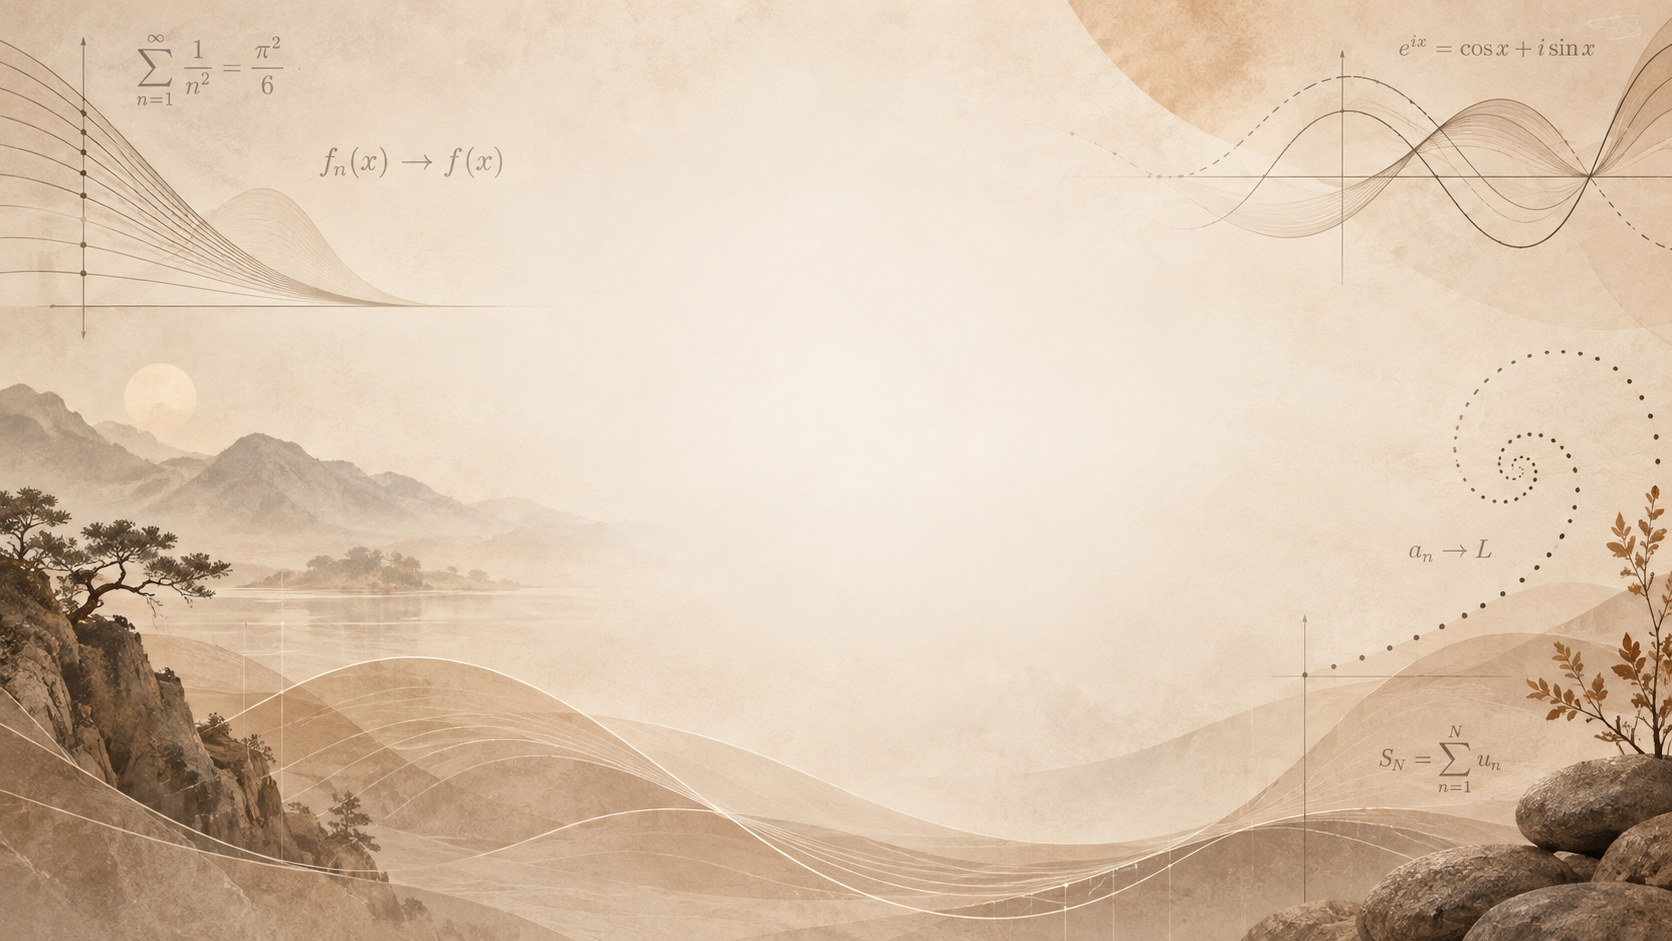
\includegraphics[width=\paperwidth,height=\paperheight,keepaspectratio=false]{chapter_07_bg_00.png}%
}
\begin{frame}[plain]
  \titlepage

  \note{
    Welcome back to Chapter 7, Sequences and Series of Functions. This is
    the seventh and final section of the chapter, The Stone Weierstrass
    Theorem. So far we have studied what happens to continuity, integrals,
    and derivatives when a sequence of functions converges uniformly. In
    this section we turn the question around. We start with a continuous
    function and ask whether it can be approximated uniformly by very simple
    functions, namely polynomials. The answer is yes, and the ideas behind
    it reach far beyond polynomials. Let's begin.
  }
\end{frame}
}

{
\usebackgroundtemplate{%
  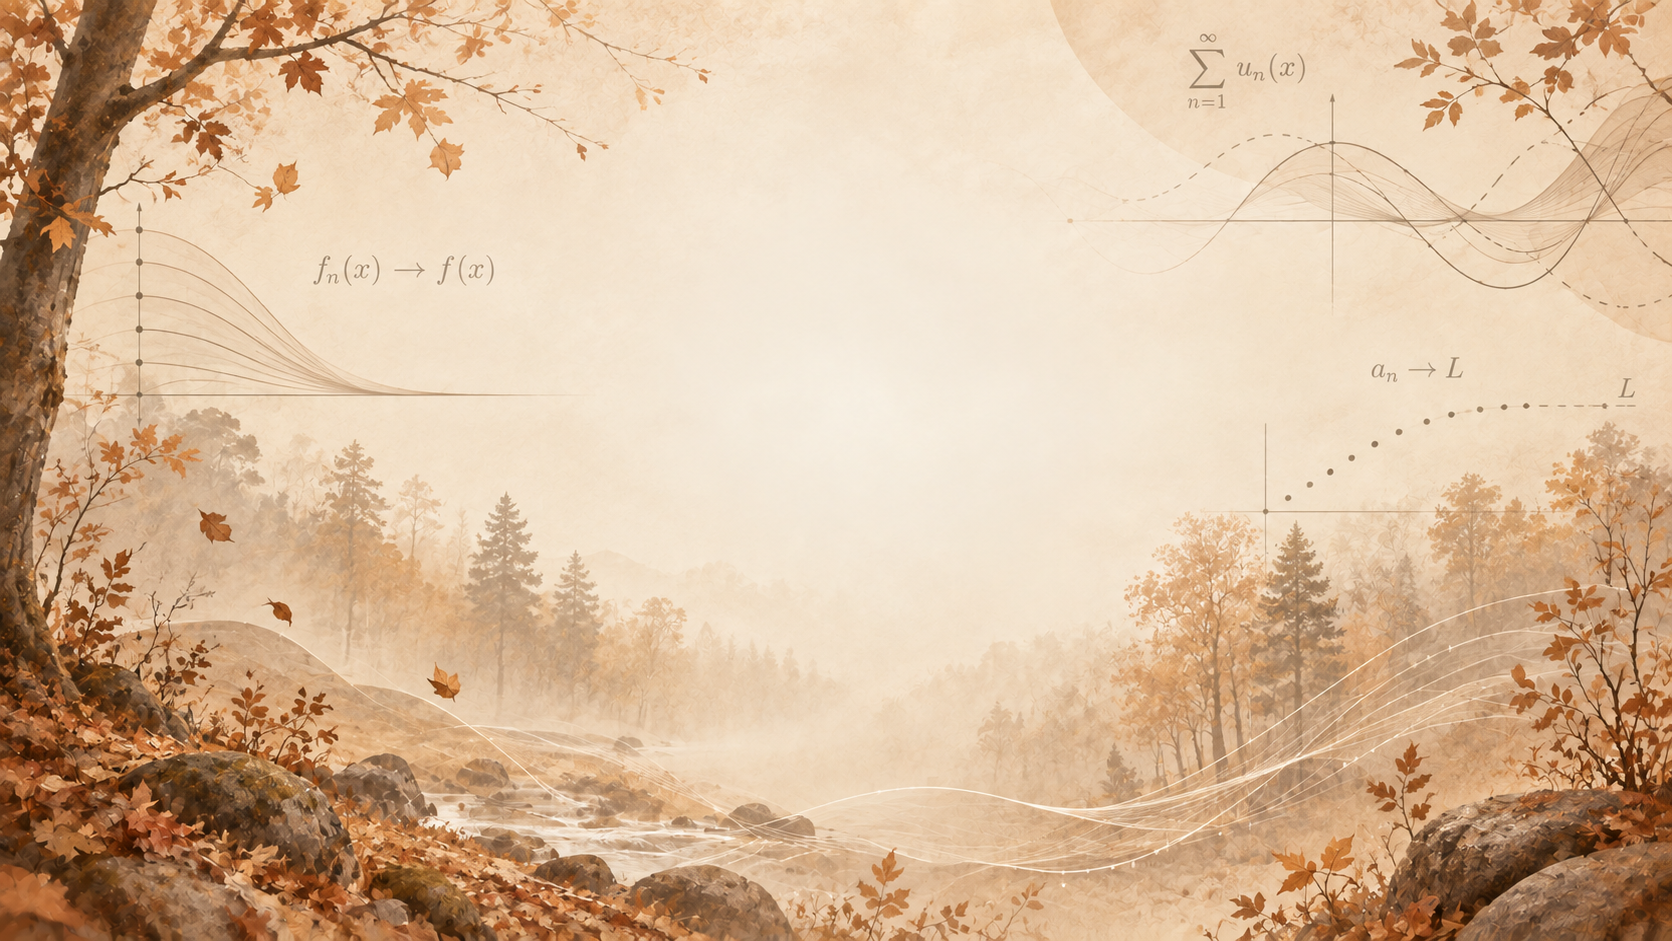
\includegraphics[width=\paperwidth,height=\paperheight,keepaspectratio=false]{chapter_07_bg_01.png}%
}
\begin{frame}[c]{Outline}
  \begin{center}
    \tableofcontents
  \end{center}

  \note{
    Here is the plan. After a short motivation, we state the Weierstrass
    approximation theorem, Theorem 7.26, and then prove it in detail. Next
    comes a small but important special case, the approximation of the
    absolute value function. We then isolate the properties of polynomials
    that make the theorem work: they form an algebra, they separate points,
    and they vanish at no point. With these in hand we prove Stone's
    generalization for real algebras, extend it to complex algebras, and
    close with a summary.
  }
\end{frame}

\section{Motivation}

% --- Build 1/4 ---
\begin{frame}{Why This Section Matters}
  \begin{hlbox}
  \begin{itemize}\setlength{\itemsep}{0.8em}
    \item So far: if $f_n \to f$ \emph{uniformly}, what does $f$ inherit from the $f_n$?
  \end{itemize}
  \end{hlbox}

  \note{
    Let's recall where we are. Throughout this chapter the sequence "f" sub
    "n" was given, and we asked what the limit function inherits. We learned
    that under uniform convergence the limit of continuous functions is
    continuous, that integrals pass to the limit, and, with extra care, so
    do derivatives. In every case, the approximating functions came first
    and the limit came second.
  }
\end{frame}

% --- Build 2/4 ---
\begin{frame}{Why This Section Matters}
  \begin{hlbox}
  \begin{itemize}\setlength{\itemsep}{0.8em}
    \item So far: if $f_n \to f$ \emph{uniformly}, what does $f$ inherit from the $f_n$?
    \item Now the reverse: given a continuous $f$, can we \alert{find} simple
      functions $f_n$ with $f_n \to f$ uniformly?
  \end{itemize}
  \end{hlbox}

  \note{
    Now we reverse the direction. Suppose a continuous function "f" is
    given, and it may be complicated. Can we find simple functions "f" sub
    "n" that converge to it uniformly? If so, then anything that survives
    uniform limits can be studied on the simple functions first and then
    transferred to "f". This is one of the most useful strategies in all of
    analysis.
  }
\end{frame}

% --- Build 3/4 ---
\begin{frame}{Why This Section Matters}
  \begin{hlbox}
  \begin{itemize}\setlength{\itemsep}{0.8em}
    \item So far: if $f_n \to f$ \emph{uniformly}, what does $f$ inherit from the $f_n$?
    \item Now the reverse: given a continuous $f$, can we \alert{find} simple
      functions $f_n$ with $f_n \to f$ uniformly?
    \item Simplest candidates: \alert{polynomials}. Taylor polynomials need
      derivatives --- but $|x|$ has none at $0$.
  \end{itemize}
  \end{hlbox}

  \note{
    The simplest functions we know are polynomials. You might think of
    Taylor polynomials, but those require the function to have derivatives
    of every order, and even then they may fail to converge to the function.
    A merely continuous function, such as the absolute value of "x", is not
    even differentiable at zero, so Taylor's theorem has nothing to say
    about it. We need a completely different way of producing polynomials.
  }
\end{frame}

% --- Build 4/4 ---
\begin{frame}{Why This Section Matters}
  \begin{hlbox}
  \begin{itemize}\setlength{\itemsep}{0.8em}
    \item So far: if $f_n \to f$ \emph{uniformly}, what does $f$ inherit from the $f_n$?
    \item Now the reverse: given a continuous $f$, can we \alert{find} simple
      functions $f_n$ with $f_n \to f$ uniformly?
    \item Simplest candidates: \alert{polynomials}. Taylor polynomials need
      derivatives --- but $|x|$ has none at $0$.
    \item Weierstrass: \alert{continuity alone is enough}.
  \end{itemize}
  \end{hlbox}

  \note{
    The remarkable answer, discovered by Weierstrass, is that continuity
    alone is enough. Every continuous function on a closed bounded interval
    is a uniform limit of polynomials. No derivatives are needed at all.
    Let's see what this statement means geometrically.
  }
\end{frame}

\begin{frame}{Uniform Approximation: The Picture}
  \begin{center}
  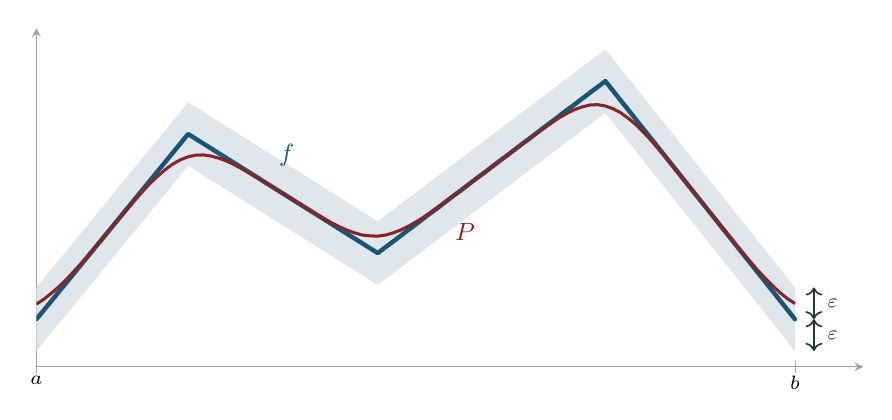
\begin{tikzpicture}
    \begin{axis}[swaxis, width=10.5cm, height=4.3cm, xmin=0, xmax=1.09, ymin=-0.18, ymax=1.1,
        xtick={0,1}, xticklabels={$a$,$b$}, ytick=\empty]
      \addplot[draw=none, fill=defcolor!14] coordinates {(0.000,0.120) (0.010,0.155) (0.020,0.190) (0.030,0.225) (0.040,0.260) (0.050,0.295) (0.060,0.330) (0.070,0.365) (0.080,0.400) (0.090,0.435) (0.100,0.470) (0.110,0.505) (0.120,0.540) (0.130,0.575) (0.140,0.610) (0.150,0.645) (0.160,0.680) (0.170,0.715) (0.180,0.750) (0.190,0.785) (0.200,0.820) (0.210,0.802) (0.220,0.784) (0.230,0.766) (0.240,0.748) (0.250,0.730) (0.260,0.712) (0.270,0.694) (0.280,0.676) (0.290,0.658) (0.300,0.640) (0.310,0.622) (0.320,0.604) (0.330,0.586) (0.340,0.568) (0.350,0.550) (0.360,0.532) (0.370,0.514) (0.380,0.496) (0.390,0.478) (0.400,0.460) (0.410,0.442) (0.420,0.424) (0.430,0.406) (0.440,0.388) (0.450,0.370) (0.460,0.392) (0.470,0.413) (0.480,0.435) (0.490,0.457) (0.500,0.478) (0.510,0.500) (0.520,0.522) (0.530,0.543) (0.540,0.565) (0.550,0.587) (0.560,0.608) (0.570,0.630) (0.580,0.652) (0.590,0.673) (0.600,0.695) (0.610,0.717) (0.620,0.738) (0.630,0.760) (0.640,0.782) (0.650,0.803) (0.660,0.825) (0.670,0.847) (0.680,0.868) (0.690,0.890) (0.700,0.912) (0.710,0.933) (0.720,0.955) (0.730,0.977) (0.740,0.998) (0.750,1.020) (0.760,0.984) (0.770,0.948) (0.780,0.912) (0.790,0.876) (0.800,0.840) (0.810,0.804) (0.820,0.768) (0.830,0.732) (0.840,0.696) (0.850,0.660) (0.860,0.624) (0.870,0.588) (0.880,0.552) (0.890,0.516) (0.900,0.480) (0.910,0.444) (0.920,0.408) (0.930,0.372) (0.940,0.336) (0.950,0.300) (0.960,0.264) (0.970,0.228) (0.980,0.192) (0.990,0.156) (1.000,0.120) (1.000,-0.120) (0.990,-0.084) (0.980,-0.048) (0.970,-0.012) (0.960,0.024) (0.950,0.060) (0.940,0.096) (0.930,0.132) (0.920,0.168) (0.910,0.204) (0.900,0.240) (0.890,0.276) (0.880,0.312) (0.870,0.348) (0.860,0.384) (0.850,0.420) (0.840,0.456) (0.830,0.492) (0.820,0.528) (0.810,0.564) (0.800,0.600) (0.790,0.636) (0.780,0.672) (0.770,0.708) (0.760,0.744) (0.750,0.780) (0.740,0.758) (0.730,0.737) (0.720,0.715) (0.710,0.693) (0.700,0.672) (0.690,0.650) (0.680,0.628) (0.670,0.607) (0.660,0.585) (0.650,0.563) (0.640,0.542) (0.630,0.520) (0.620,0.498) (0.610,0.477) (0.600,0.455) (0.590,0.433) (0.580,0.412) (0.570,0.390) (0.560,0.368) (0.550,0.347) (0.540,0.325) (0.530,0.303) (0.520,0.282) (0.510,0.260) (0.500,0.238) (0.490,0.217) (0.480,0.195) (0.470,0.173) (0.460,0.152) (0.450,0.130) (0.440,0.148) (0.430,0.166) (0.420,0.184) (0.410,0.202) (0.400,0.220) (0.390,0.238) (0.380,0.256) (0.370,0.274) (0.360,0.292) (0.350,0.310) (0.340,0.328) (0.330,0.346) (0.320,0.364) (0.310,0.382) (0.300,0.400) (0.290,0.418) (0.280,0.436) (0.270,0.454) (0.260,0.472) (0.250,0.490) (0.240,0.508) (0.230,0.526) (0.220,0.544) (0.210,0.562) (0.200,0.580) (0.190,0.545) (0.180,0.510) (0.170,0.475) (0.160,0.440) (0.150,0.405) (0.140,0.370) (0.130,0.335) (0.120,0.300) (0.110,0.265) (0.100,0.230) (0.090,0.195) (0.080,0.160) (0.070,0.125) (0.060,0.090) (0.050,0.055) (0.040,0.020) (0.030,-0.015) (0.020,-0.050) (0.010,-0.085) (0.000,-0.120)} -- cycle;
      \addplot[defcolor, curveln] coordinates {(0.000,0.000) (0.010,0.035) (0.020,0.070) (0.030,0.105) (0.040,0.140) (0.050,0.175) (0.060,0.210) (0.070,0.245) (0.080,0.280) (0.090,0.315) (0.100,0.350) (0.110,0.385) (0.120,0.420) (0.130,0.455) (0.140,0.490) (0.150,0.525) (0.160,0.560) (0.170,0.595) (0.180,0.630) (0.190,0.665) (0.200,0.700) (0.210,0.682) (0.220,0.664) (0.230,0.646) (0.240,0.628) (0.250,0.610) (0.260,0.592) (0.270,0.574) (0.280,0.556) (0.290,0.538) (0.300,0.520) (0.310,0.502) (0.320,0.484) (0.330,0.466) (0.340,0.448) (0.350,0.430) (0.360,0.412) (0.370,0.394) (0.380,0.376) (0.390,0.358) (0.400,0.340) (0.410,0.322) (0.420,0.304) (0.430,0.286) (0.440,0.268) (0.450,0.250) (0.460,0.272) (0.470,0.293) (0.480,0.315) (0.490,0.337) (0.500,0.358) (0.510,0.380) (0.520,0.402) (0.530,0.423) (0.540,0.445) (0.550,0.467) (0.560,0.488) (0.570,0.510) (0.580,0.532) (0.590,0.553) (0.600,0.575) (0.610,0.597) (0.620,0.618) (0.630,0.640) (0.640,0.662) (0.650,0.683) (0.660,0.705) (0.670,0.727) (0.680,0.748) (0.690,0.770) (0.700,0.792) (0.710,0.813) (0.720,0.835) (0.730,0.857) (0.740,0.878) (0.750,0.900) (0.760,0.864) (0.770,0.828) (0.780,0.792) (0.790,0.756) (0.800,0.720) (0.810,0.684) (0.820,0.648) (0.830,0.612) (0.840,0.576) (0.850,0.540) (0.860,0.504) (0.870,0.468) (0.880,0.432) (0.890,0.396) (0.900,0.360) (0.910,0.324) (0.920,0.288) (0.930,0.252) (0.940,0.216) (0.950,0.180) (0.960,0.144) (0.970,0.108) (0.980,0.072) (0.990,0.036) (1.000,0.000)};
      \addplot[thmcolor, line width=1.1pt] coordinates {(0.000,0.057) (0.010,0.076) (0.020,0.099) (0.030,0.124) (0.040,0.152) (0.050,0.183) (0.060,0.214) (0.070,0.247) (0.080,0.281) (0.090,0.315) (0.100,0.350) (0.110,0.384) (0.120,0.418) (0.130,0.451) (0.140,0.483) (0.150,0.514) (0.160,0.541) (0.170,0.566) (0.180,0.587) (0.190,0.603) (0.200,0.614) (0.210,0.620) (0.220,0.621) (0.230,0.617) (0.240,0.609) (0.250,0.599) (0.260,0.585) (0.270,0.570) (0.280,0.554) (0.290,0.537) (0.300,0.520) (0.310,0.502) (0.320,0.484) (0.330,0.466) (0.340,0.448) (0.350,0.430) (0.360,0.413) (0.370,0.395) (0.380,0.379) (0.390,0.363) (0.400,0.349) (0.410,0.336) (0.420,0.326) (0.430,0.318) (0.440,0.315) (0.450,0.314) (0.460,0.318) (0.470,0.326) (0.480,0.337) (0.490,0.351) (0.500,0.367) (0.510,0.385) (0.520,0.404) (0.530,0.425) (0.540,0.446) (0.550,0.467) (0.560,0.488) (0.570,0.510) (0.580,0.532) (0.590,0.553) (0.600,0.575) (0.610,0.597) (0.620,0.618) (0.630,0.640) (0.640,0.661) (0.650,0.683) (0.660,0.704) (0.670,0.724) (0.680,0.744) (0.690,0.763) (0.700,0.779) (0.710,0.793) (0.720,0.803) (0.730,0.810) (0.740,0.811) (0.750,0.806) (0.760,0.796) (0.770,0.781) (0.780,0.760) (0.790,0.736) (0.800,0.708) (0.810,0.677) (0.820,0.644) (0.830,0.610) (0.840,0.575) (0.850,0.539) (0.860,0.504) (0.870,0.468) (0.880,0.432) (0.890,0.396) (0.900,0.360) (0.910,0.325) (0.920,0.289) (0.930,0.255) (0.940,0.221) (0.950,0.188) (0.960,0.157) (0.970,0.128) (0.980,0.101) (0.990,0.078) (1.000,0.059)};
      \node[defcolor, font=\small] at (axis cs:0.33,0.62) {$f$};
      \node[thmcolor, font=\small] at (axis cs:0.565,0.33) {$P$};
      \draw[<->, mDarkTeal, line width=0.6pt] (axis cs:1.025,0) -- (axis cs:1.025,0.12);
      \draw[<->, mDarkTeal, line width=0.6pt] (axis cs:1.025,0) -- (axis cs:1.025,-0.12);
      \node[mDarkTeal, font=\scriptsize, anchor=west] at (axis cs:1.03,0.06) {$\varepsilon$};
      \node[mDarkTeal, font=\scriptsize, anchor=west] at (axis cs:1.03,-0.06) {$\varepsilon$};
    \end{axis}
  \end{tikzpicture}

  \smallskip
  \begin{hlbox}
  \centering
  $|P(x) - f(x)| < \varepsilon$ for \alert{all} $x \in [a,b]$:
  the graph of $P$ stays inside the $\varepsilon$-tube around $f$.
  \end{hlbox}
  \end{center}

  \note{
    Look at the picture. The blue zigzag is a continuous function "f" on the
    interval from "a" to "b". It has sharp corners, so it is certainly not
    differentiable everywhere. The light blue band around it is the epsilon
    tube: all points within vertical distance epsilon of the graph. The red
    curve is a polynomial, capital "P", which was actually computed by the
    method of this section. It rounds off the corners, but it never leaves
    the band. That is exactly what the inequality under the picture says:
    the distance between capital "P" of "x" and "f" of "x" is less than
    epsilon at every point "x" simultaneously. The Weierstrass theorem
    promises such a polynomial for every epsilon, no matter how thin the
    tube.
  }
\end{frame}

% --- Build 1/3 ---
\begin{frame}{Roadmap}
  \begin{hlbox}
  \begin{itemize}\setlength{\itemsep}{0.9em}
    \item \textbf{Theorem 7.26 (Weierstrass):} polynomials approximate every
      continuous function on $[a,b]$ uniformly
  \end{itemize}
  \end{hlbox}

  \note{
    Here is the road ahead, in three stages. The first stage is the
    Weierstrass theorem itself, Theorem 7.26. We will prove it with an
    explicit construction: the approximating polynomials are obtained by
    averaging "f" against a sequence of sharply peaked polynomial kernels.
  }
\end{frame}

% --- Build 2/3 ---
\begin{frame}{Roadmap}
  \begin{hlbox}
  \begin{itemize}\setlength{\itemsep}{0.9em}
    \item \textbf{Theorem 7.26 (Weierstrass):} polynomials approximate every
      continuous function on $[a,b]$ uniformly
    \item \textbf{7.28--7.31:} what makes polynomials work? They form an
      \alert{algebra} that \alert{separates points} and \alert{vanishes at no point}
  \end{itemize}
  \end{hlbox}

  \note{
    In the second stage we ask what is special about polynomials. It turns
    out that only three structural properties matter. Polynomials form an
    algebra, which means sums, products, and constant multiples of
    polynomials are again polynomials. They separate points, and they vanish
    at no point. We will define these notions carefully in Definitions 7.28
    and 7.30.
  }
\end{frame}

% --- Build 3/3 ---
\begin{frame}{Roadmap}
  \begin{hlbox}
  \begin{itemize}\setlength{\itemsep}{0.9em}
    \item \textbf{Theorem 7.26 (Weierstrass):} polynomials approximate every
      continuous function on $[a,b]$ uniformly
    \item \textbf{7.28--7.31:} what makes polynomials work? They form an
      \alert{algebra} that \alert{separates points} and \alert{vanishes at no point}
    \item \textbf{Theorems 7.32, 7.33 (Stone):} \emph{any} such algebra of continuous
      functions on a compact set $K$ is dense in $\mathscr{C}(K)$
  \end{itemize}
  \end{hlbox}

  \note{
    The third stage is Stone's generalization. Any algebra of continuous
    functions on a compact set capital "K" with those properties can
    approximate every continuous function on capital "K" uniformly. Theorem
    7.32 treats real functions, and Theorem 7.33 treats complex functions,
    where one extra condition is needed. So the interval is replaced by an
    arbitrary compact set, and the polynomials by an abstract algebra. Let's
    start with the classical theorem.
  }
\end{frame}
}

{
\usebackgroundtemplate{%
  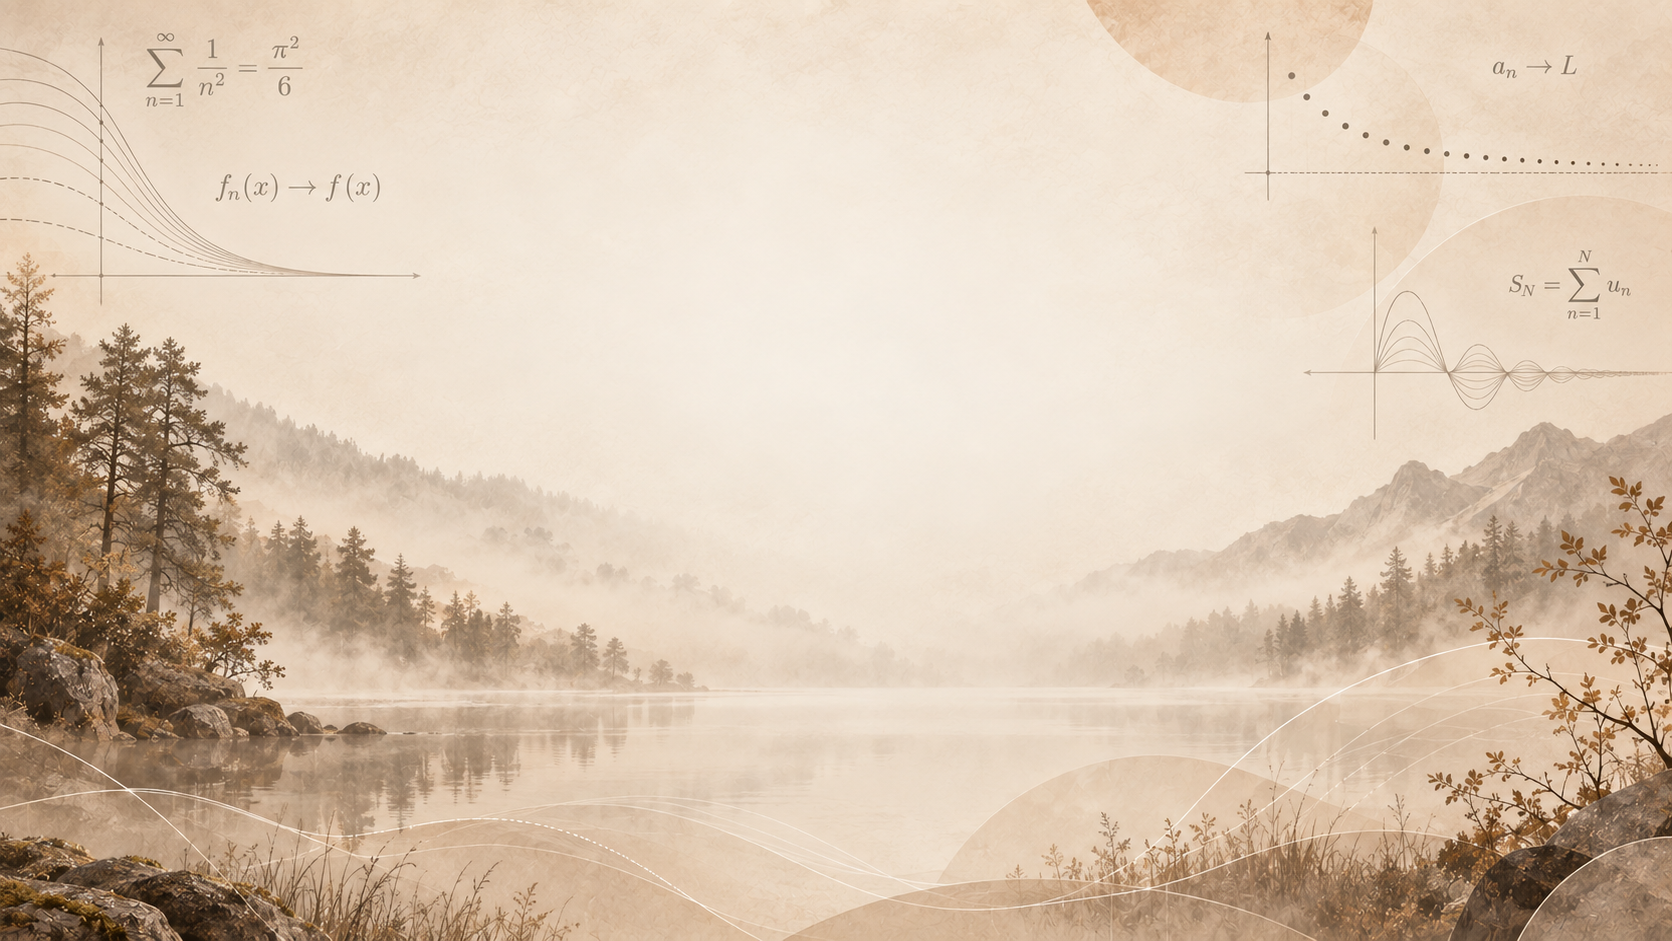
\includegraphics[width=\paperwidth,height=\paperheight,keepaspectratio=false]{chapter_07_bg_02.png}%
}
\section{The Weierstrass Theorem}

% --- Build 1/2 ---
\begin{frame}{Theorem 7.26: The Weierstrass Approximation Theorem}
  \begin{thmblock}{Theorem 7.26}
    If $f$ is a continuous complex function on $[a,b]$, there exists a sequence of
    polynomials $P_n$ such that
    \[
      \lim_{n \to \infty} P_n(x) = f(x)
    \]
    uniformly on $[a,b]$. If $f$ is real, the $P_n$ may be taken real.
  \end{thmblock}

  \hl{\small This is the form in which the theorem was originally discovered by Weierstrass.}

  \note{
    Here is the precise statement. Let "f" be a continuous complex valued
    function on the closed interval from "a" to "b". Then there is a
    sequence of polynomials, capital "P" sub "n", converging to "f"
    uniformly on that interval. If "f" is real valued, the polynomials can
    be chosen with real coefficients. As the line under the theorem says,
    this is the form in which Weierstrass originally discovered the result.
    Notice that the interval is closed and bounded, so it is compact. That
    will matter, because the proof uses uniform continuity.
  }
\end{frame}

% --- Build 2/2 ---
\begin{frame}{Theorem 7.26: The Weierstrass Approximation Theorem}
  \begin{thmblock}{Theorem 7.26}
    If $f$ is a continuous complex function on $[a,b]$, there exists a sequence of
    polynomials $P_n$ such that
    \[
      \lim_{n \to \infty} P_n(x) = f(x)
    \]
    uniformly on $[a,b]$. If $f$ is real, the $P_n$ may be taken real.
  \end{thmblock}

  \hl{\small This is the form in which the theorem was originally discovered by Weierstrass.}

  \vspace{0.2em}
  \begin{hlbox}
  \textbf{Equivalently:} for every $\varepsilon > 0$ there is a polynomial $P$ with
  \[
    \sup_{a \le x \le b} |P(x) - f(x)| < \varepsilon .
  \]
  \end{hlbox}

  \note{
    The theorem can be restated without sequences. For every epsilon there
    is a single polynomial capital "P" whose distance from "f", measured by
    the supremum over the whole interval, is less than epsilon. The two
    versions are equivalent. Given the sequence, take a term far enough out.
    Conversely, given such a polynomial for epsilon equal to 1 over "n", for
    each "n", line them up into a sequence. This is the tube picture from
    the motivation. Before the details, let's look at the overall strategy.
  }
\end{frame}

% --- Build 1/4 ---
\begin{frame}{Proof Strategy: Theorem 7.26}
  \begin{hlbox}
  \textbf{Goal:} polynomials $P_n \to f$ uniformly on $[a,b]$.

  \vspace{0.6em}
  \textbf{Approach:}
  \begin{enumerate}\setlength{\itemsep}{0.5em}
    \item \textbf{Normalize:} reduce to $[0,1]$ with $f(0) = f(1) = 0$; extend $f$ by $0$.
  \end{enumerate}
  \end{hlbox}

  \note{
    The proof has four parts. First, we normalize. We will see that it is
    enough to treat the interval from 0 to 1, and a function that vanishes
    at both endpoints. Such a function can be extended by zero to the whole
    real line and stays continuous. This costs nothing and makes the later
    formulas clean.
  }
\end{frame}

% --- Build 2/4 ---
\begin{frame}{Proof Strategy: Theorem 7.26}
  \begin{hlbox}
  \textbf{Goal:} polynomials $P_n \to f$ uniformly on $[a,b]$.

  \vspace{0.6em}
  \textbf{Approach:}
  \begin{enumerate}\setlength{\itemsep}{0.5em}
    \item \textbf{Normalize:} reduce to $[0,1]$ with $f(0) = f(1) = 0$; extend $f$ by $0$.
    \item \textbf{Kernel:} polynomials $Q_n \ge 0$ with $\int_{-1}^{1} Q_n = 1$,
      concentrated near $0$.
  \end{enumerate}
  \end{hlbox}

  \note{
    Second, we build a kernel. This is a sequence of polynomials capital "Q"
    sub "n" which are nonnegative, have total integral 1 over the interval
    from minus 1 to 1, and concentrate more and more of their area near zero
    as "n" grows. You can think of them as sharper and sharper bumps.
  }
\end{frame}

% --- Build 3/4 ---
\begin{frame}{Proof Strategy: Theorem 7.26}
  \begin{hlbox}
  \textbf{Goal:} polynomials $P_n \to f$ uniformly on $[a,b]$.

  \vspace{0.6em}
  \textbf{Approach:}
  \begin{enumerate}\setlength{\itemsep}{0.5em}
    \item \textbf{Normalize:} reduce to $[0,1]$ with $f(0) = f(1) = 0$; extend $f$ by $0$.
    \item \textbf{Kernel:} polynomials $Q_n \ge 0$ with $\int_{-1}^{1} Q_n = 1$,
      concentrated near $0$.
    \item \textbf{Average:} $P_n(x) = \int_{-1}^{1} f(x+t)\,Q_n(t)\,dt$ is a polynomial.
  \end{enumerate}
  \end{hlbox}

  \note{
    Third, we average. The function capital "P" sub "n" at the point "x" is
    a weighted average of the values of "f" near "x", with weights given by
    the bump capital "Q" sub "n". The surprise is that this average is
    itself a polynomial in "x". The polynomial nature of the kernel is
    inherited by the average.
  }
\end{frame}

% --- Build 4/4 ---
\begin{frame}{Proof Strategy: Theorem 7.26}
  \begin{hlbox}
  \textbf{Goal:} polynomials $P_n \to f$ uniformly on $[a,b]$.

  \vspace{0.6em}
  \textbf{Approach:}
  \begin{enumerate}\setlength{\itemsep}{0.5em}
    \item \textbf{Normalize:} reduce to $[0,1]$ with $f(0) = f(1) = 0$; extend $f$ by $0$.
    \item \textbf{Kernel:} polynomials $Q_n \ge 0$ with $\int_{-1}^{1} Q_n = 1$,
      concentrated near $0$.
    \item \textbf{Average:} $P_n(x) = \int_{-1}^{1} f(x+t)\,Q_n(t)\,dt$ is a polynomial.
    \item \textbf{Estimate:} split the integral into $|t| < \delta$ (where $f$ barely
      changes) and $|t| \ge \delta$ (where $Q_n$ is tiny).
  \end{enumerate}
  \end{hlbox}

  \note{
    Fourth, we estimate the error. We split the integral into two regions.
    For small "t", with absolute value below delta, uniform continuity says
    that "f" barely changes. For "t" at distance at least delta from zero,
    the kernel is tiny. Both contributions are small, uniformly in "x". This
    split into a near part and a far part is a classical technique that
    reappears throughout analysis. Let's carry out the four parts in order.
  }
\end{frame}
}

{
\usebackgroundtemplate{%
  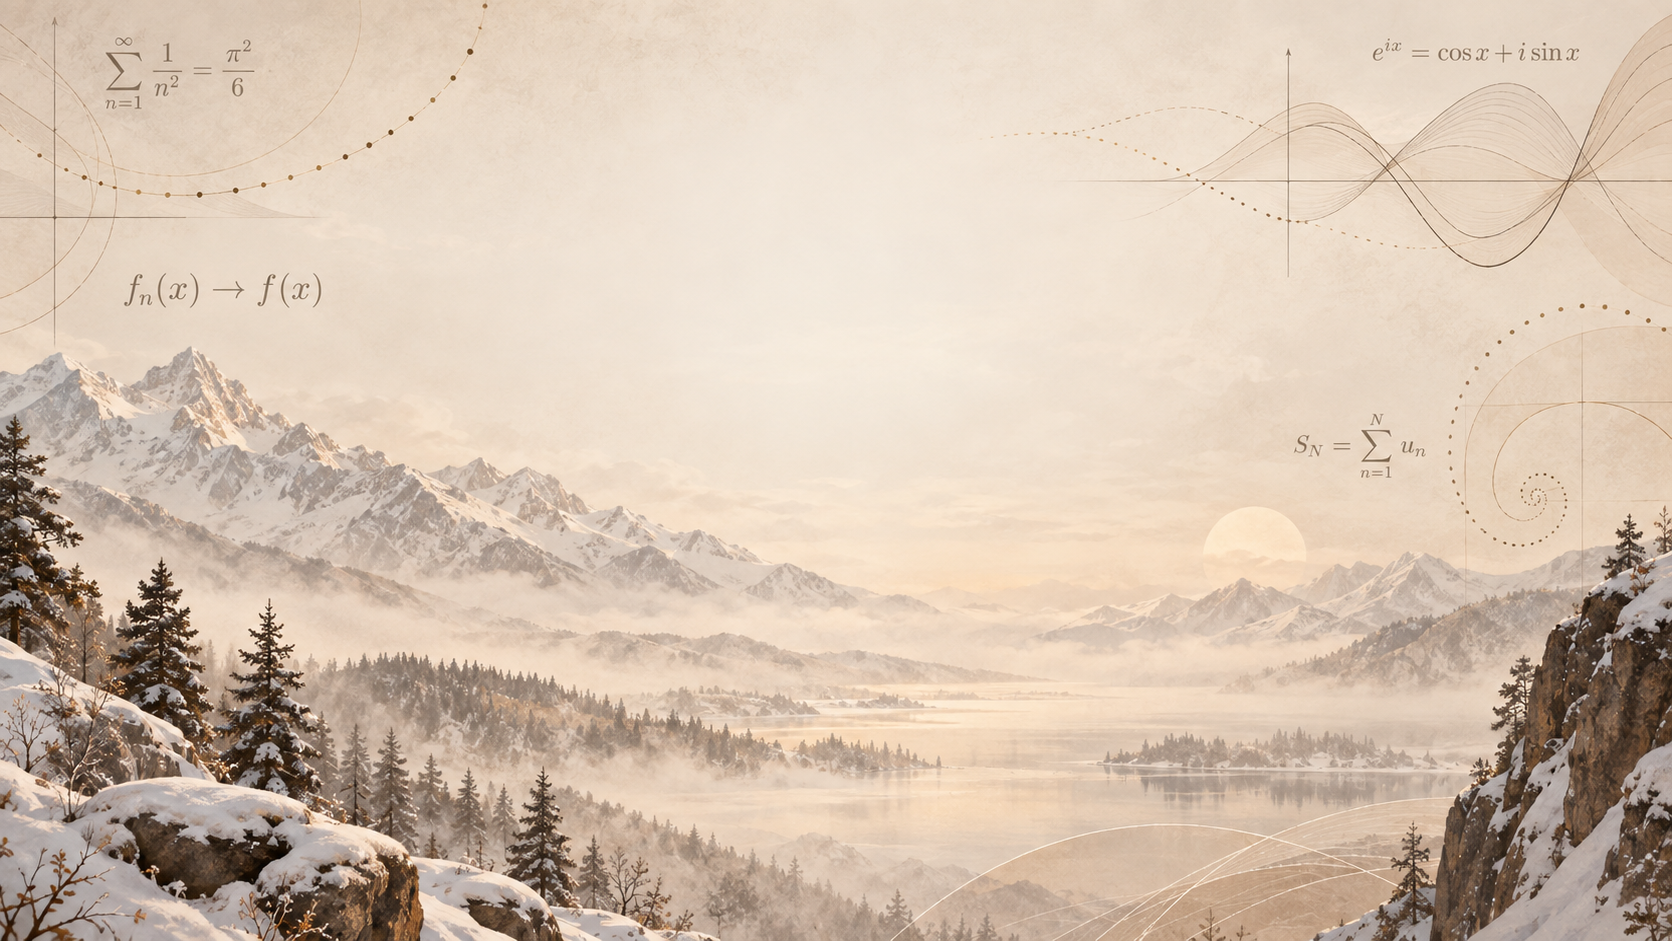
\includegraphics[width=\paperwidth,height=\paperheight,keepaspectratio=false]{chapter_07_bg_03.png}%
}
\section{Proof of the Weierstrass Theorem}

% --- Build 1/3 ---
\begin{frame}{Proof of Theorem 7.26 --- Reductions}
  \begin{columns}[T]
    \begin{column}{0.54\textwidth}
      \small
      \begin{proofblock}{Reduction 1: the interval}
        We may assume $[a,b] = [0,1]$. \;{\footnotesize\\
        Rescale: $x = a + (b-a)s$}.
      \end{proofblock}
    \end{column}
    \begin{column}{0.44\textwidth}
      \centering
  \vspace{1.5em}
  \begin{tikzpicture}
    \begin{axis}[swaxis, width=5.6cm, height=3.6cm, xmin=-0.6, xmax=1.6, ymin=0, ymax=1.15,
        xtick={0,1}, ytick=\empty]
      \addplot[defcolor, curveln] coordinates {(0.000,0.350) (0.013,0.384) (0.025,0.419) (0.037,0.452) (0.050,0.485) (0.062,0.517) (0.075,0.547) (0.087,0.577) (0.100,0.604) (0.113,0.630) (0.125,0.653) (0.138,0.675) (0.150,0.694) (0.163,0.711) (0.175,0.726) (0.188,0.739) (0.200,0.749) (0.212,0.757) (0.225,0.763) (0.237,0.766) (0.250,0.768) (0.263,0.768) (0.275,0.766) (0.287,0.763) (0.300,0.759) (0.312,0.754) (0.325,0.748) (0.338,0.741) (0.350,0.734) (0.362,0.727) (0.375,0.720) (0.388,0.713) (0.400,0.707) (0.412,0.702) (0.425,0.698) (0.438,0.695) (0.450,0.693) (0.463,0.692) (0.475,0.693) (0.487,0.696) (0.500,0.700) (0.512,0.706) (0.525,0.713) (0.537,0.722) (0.550,0.733) (0.562,0.745) (0.575,0.758) (0.588,0.772) (0.600,0.787) (0.613,0.803) (0.625,0.820) (0.637,0.837) (0.650,0.854) (0.662,0.871) (0.675,0.888) (0.688,0.904) (0.700,0.919) (0.713,0.933) (0.725,0.946) (0.738,0.958) (0.750,0.968) (0.762,0.976) (0.775,0.983) (0.787,0.987) (0.800,0.989) (0.812,0.989) (0.825,0.986) (0.838,0.981) (0.850,0.974) (0.863,0.965) (0.875,0.953) (0.887,0.940) (0.900,0.924) (0.912,0.907) (0.925,0.887) (0.938,0.867) (0.950,0.845) (0.963,0.822) (0.975,0.799) (0.988,0.774) (1.000,0.750)};
      \node[defcolor, font=\small] at (axis cs:0.5,0.88) {$f$};
    \end{axis}
  \end{tikzpicture}
    \end{column}
  \end{columns}

  \note{
    We begin with the reductions. Without loss of generality the interval is
    the unit interval from 0 to 1. The reason is the linear change of
    variable shown in small print. It maps the unit interval onto the
    interval from "a" to "b", and composing a polynomial with a linear map
    gives another polynomial. So a uniform approximation on one interval
    transfers to the other. On the right you see a typical continuous
    function "f" on the unit interval, drawn in blue.
  }
\end{frame}

% --- Build 2/3 ---
\begin{frame}{Proof of Theorem 7.26 --- Reductions}
  \begin{columns}[T]
    \begin{column}{0.54\textwidth}
      \small
      \begin{proofblock}{Reduction 1: the interval}
        We may assume $[a,b] = [0,1]$. \;{\footnotesize\\
        Rescale: $x = a + (b-a)s$}.
      \end{proofblock}
      \begin{proofblock}{Reduction 2: the endpoints}
        We may assume $f(0) = f(1) = 0$. Otherwise use
        \[
          g(x) = f(x) - f(0) - x\,[f(1) - f(0)] :
        \]
        $g(0) = g(1) = 0$, and $f - g$ is a polynomial.
      \end{proofblock}
    \end{column}
    \begin{column}{0.44\textwidth}
      \centering
  \vspace{1.5em}
  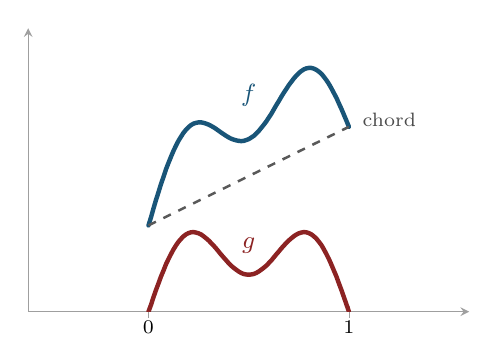
\begin{tikzpicture}
    \begin{axis}[swaxis, width=5.6cm, height=3.6cm, xmin=-0.6, xmax=1.6, ymin=0, ymax=1.15,
        xtick={0,1}, ytick=\empty]
      \addplot[defcolor, curveln] coordinates {(0.000,0.350) (0.013,0.384) (0.025,0.419) (0.037,0.452) (0.050,0.485) (0.062,0.517) (0.075,0.547) (0.087,0.577) (0.100,0.604) (0.113,0.630) (0.125,0.653) (0.138,0.675) (0.150,0.694) (0.163,0.711) (0.175,0.726) (0.188,0.739) (0.200,0.749) (0.212,0.757) (0.225,0.763) (0.237,0.766) (0.250,0.768) (0.263,0.768) (0.275,0.766) (0.287,0.763) (0.300,0.759) (0.312,0.754) (0.325,0.748) (0.338,0.741) (0.350,0.734) (0.362,0.727) (0.375,0.720) (0.388,0.713) (0.400,0.707) (0.412,0.702) (0.425,0.698) (0.438,0.695) (0.450,0.693) (0.463,0.692) (0.475,0.693) (0.487,0.696) (0.500,0.700) (0.512,0.706) (0.525,0.713) (0.537,0.722) (0.550,0.733) (0.562,0.745) (0.575,0.758) (0.588,0.772) (0.600,0.787) (0.613,0.803) (0.625,0.820) (0.637,0.837) (0.650,0.854) (0.662,0.871) (0.675,0.888) (0.688,0.904) (0.700,0.919) (0.713,0.933) (0.725,0.946) (0.738,0.958) (0.750,0.968) (0.762,0.976) (0.775,0.983) (0.787,0.987) (0.800,0.989) (0.812,0.989) (0.825,0.986) (0.838,0.981) (0.850,0.974) (0.863,0.965) (0.875,0.953) (0.887,0.940) (0.900,0.924) (0.912,0.907) (0.925,0.887) (0.938,0.867) (0.950,0.845) (0.963,0.822) (0.975,0.799) (0.988,0.774) (1.000,0.750)};
      \node[defcolor, font=\small] at (axis cs:0.5,0.88) {$f$};
      \addplot[gray!70!black, dashed, line width=0.9pt] coordinates {(0,0.35) (1,0.75)};
      \addplot[thmcolor, curveln] coordinates {(0.000,0.000) (0.013,0.029) (0.025,0.059) (0.037,0.087) (0.050,0.115) (0.062,0.142) (0.075,0.167) (0.087,0.192) (0.100,0.214) (0.113,0.235) (0.125,0.253) (0.138,0.270) (0.150,0.284) (0.163,0.296) (0.175,0.306) (0.188,0.314) (0.200,0.319) (0.212,0.322) (0.225,0.323) (0.237,0.321) (0.250,0.318) (0.263,0.313) (0.275,0.306) (0.287,0.298) (0.300,0.289) (0.312,0.279) (0.325,0.268) (0.338,0.256) (0.350,0.244) (0.362,0.232) (0.375,0.220) (0.388,0.208) (0.400,0.197) (0.412,0.187) (0.425,0.178) (0.438,0.170) (0.450,0.163) (0.463,0.157) (0.475,0.153) (0.487,0.151) (0.500,0.150) (0.512,0.151) (0.525,0.153) (0.537,0.157) (0.550,0.163) (0.562,0.170) (0.575,0.178) (0.588,0.187) (0.600,0.197) (0.613,0.208) (0.625,0.220) (0.637,0.232) (0.650,0.244) (0.662,0.256) (0.675,0.268) (0.688,0.279) (0.700,0.289) (0.713,0.298) (0.725,0.306) (0.738,0.313) (0.750,0.318) (0.762,0.321) (0.775,0.323) (0.787,0.322) (0.800,0.319) (0.812,0.314) (0.825,0.306) (0.838,0.296) (0.850,0.284) (0.863,0.270) (0.875,0.253) (0.887,0.235) (0.900,0.214) (0.912,0.192) (0.925,0.167) (0.938,0.142) (0.950,0.115) (0.963,0.087) (0.975,0.059) (0.988,0.029) (1.000,0.000)};
      \node[thmcolor, font=\small] at (axis cs:0.5,0.27) {$g$};
      \node[gray!60!black, font=\scriptsize, anchor=west] at (axis cs:1.02,0.78) {chord};
    \end{axis}
  \end{tikzpicture}
    \end{column}
  \end{columns}

  \note{
    Second, we may assume that "f" vanishes at both endpoints. If it does
    not, subtract from "f" the linear function that matches it at 0 and at
    1. In the picture, that linear function is the dashed gray chord, and
    the difference is the red curve "g". By construction "g" is zero at both
    endpoints. If polynomials converge uniformly to "g", then adding the
    chord back gives polynomials converging uniformly to "f", because "f"
    minus "g" is itself a polynomial of degree one. So it suffices to prove
    the theorem for "g".
  }
\end{frame}

% --- Build 3/3 ---
\begin{frame}{Proof of Theorem 7.26 --- Reductions}
  \begin{columns}[T]
    \begin{column}{0.54\textwidth}
      \small
      \begin{proofblock}{Reduction 1: the interval}
        We may assume $[a,b] = [0,1]$. \;{\footnotesize\\
        Rescale: $x = a + (b-a)s$}.
      \end{proofblock}
      \begin{proofblock}{Reduction 2: the endpoints}
        We may assume $f(0) = f(1) = 0$. Otherwise use
        \[
          g(x) = f(x) - f(0) - x\,[f(1) - f(0)] :
        \]
        $g(0) = g(1) = 0$, and $f - g$ is a polynomial.
      \end{proofblock}
      \begin{proofblock}{Extension}
        Define $f(x) = 0$ for $x$ outside $[0,1]$.\\
        Then $f$ is \alert{uniformly continuous} on $\mathbb{R}$.
      \end{proofblock}
    \end{column}
    \begin{column}{0.44\textwidth}
      \centering
  \vspace{1.5em}
  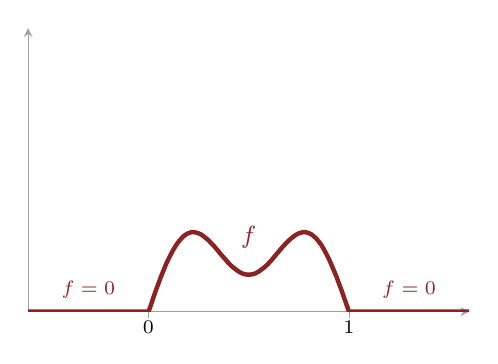
\begin{tikzpicture}
    \begin{axis}[swaxis, width=5.6cm, height=3.6cm, xmin=-0.6, xmax=1.6, ymin=0, ymax=1.15,
        xtick={0,1}, ytick=\empty]
      \addplot[thmcolor, curveln] coordinates {(-0.6,0) (0,0) (0.000,0.000) (0.013,0.029) (0.025,0.059) (0.037,0.087) (0.050,0.115) (0.062,0.142) (0.075,0.167) (0.087,0.192) (0.100,0.214) (0.113,0.235) (0.125,0.253) (0.138,0.270) (0.150,0.284) (0.163,0.296) (0.175,0.306) (0.188,0.314) (0.200,0.319) (0.212,0.322) (0.225,0.323) (0.237,0.321) (0.250,0.318) (0.263,0.313) (0.275,0.306) (0.287,0.298) (0.300,0.289) (0.312,0.279) (0.325,0.268) (0.338,0.256) (0.350,0.244) (0.362,0.232) (0.375,0.220) (0.388,0.208) (0.400,0.197) (0.412,0.187) (0.425,0.178) (0.438,0.170) (0.450,0.163) (0.463,0.157) (0.475,0.153) (0.487,0.151) (0.500,0.150) (0.512,0.151) (0.525,0.153) (0.537,0.157) (0.550,0.163) (0.562,0.170) (0.575,0.178) (0.588,0.187) (0.600,0.197) (0.613,0.208) (0.625,0.220) (0.637,0.232) (0.650,0.244) (0.662,0.256) (0.675,0.268) (0.688,0.279) (0.700,0.289) (0.713,0.298) (0.725,0.306) (0.738,0.313) (0.750,0.318) (0.762,0.321) (0.775,0.323) (0.787,0.322) (0.800,0.319) (0.812,0.314) (0.825,0.306) (0.838,0.296) (0.850,0.284) (0.863,0.270) (0.875,0.253) (0.887,0.235) (0.900,0.214) (0.912,0.192) (0.925,0.167) (0.938,0.142) (0.950,0.115) (0.963,0.087) (0.975,0.059) (0.988,0.029) (1.000,0.000) (1,0) (1.6,0)};
      \node[thmcolor, font=\small] at (axis cs:0.5,0.3) {$f$};
      \node[thmcolor, font=\scriptsize] at (axis cs:-0.3,0.09) {$f = 0$};
      \node[thmcolor, font=\scriptsize] at (axis cs:1.3,0.09) {$f = 0$};
    \end{axis}
  \end{tikzpicture}
    \end{column}
  \end{columns}

  \note{
    From now on we call the reduced function "f" again. Since it vanishes at
    0 and at 1, we can extend it to the whole real line by setting it equal
    to zero outside the unit interval, as the red curve in the picture
    shows. There is no jump at the endpoints, so the extension is
    continuous. It is uniformly continuous on the unit interval by
    compactness, and constant outside, so it is uniformly continuous on the
    whole line. This is why we wanted zero boundary values. Next we
    construct the kernel.
  }
\end{frame}

% --- Build 1/2 ---
\begin{frame}{Proof of Theorem 7.26 --- The Kernel $Q_n$}
  \begin{columns}[T]
    \begin{column}{0.42\textwidth}
      \begin{proofblock}{The polynomials $Q_n$}
        For $n = 1, 2, 3, \dots$ put
        \[
          Q_n(x) = c_n (1 - x^2)^n , \tag{47}
        \]
        where $c_n$ is chosen so that
        \[
          \int_{-1}^{1} Q_n(x)\,dx = 1 . \tag{48}
        \]
      \end{proofblock}
    \end{column}
    \begin{column}{0.56\textwidth}
      \centering

    \end{column}
  \end{columns}

  \note{
    Here is the kernel. For each positive integer "n", capital "Q" sub "n"
    of "x" is a constant "c" sub "n" times the quantity 1 minus "x" squared,
    raised to the power "n". This is equation 47. The quantity 1 minus "x"
    squared is the simplest polynomial bump: it equals 1 at the center and
    drops to 0 at minus 1 and at 1. So capital "Q" sub "n" is a polynomial
    of degree 2 times "n". The constant "c" sub "n" is a normalization. It
    is chosen so that the integral of capital "Q" sub "n" from minus 1 to 1
    equals 1, which is equation 48. Let's see what these functions look
    like.
  }
\end{frame}

% --- Build 2/2 ---
\begin{frame}{Proof of Theorem 7.26 --- The Kernel $Q_n$}
  \begin{columns}[T]
    \begin{column}{0.42\textwidth}
      \begin{proofblock}{The polynomials $Q_n$}
        For $n = 1, 2, 3, \dots$ put
        \[
          Q_n(x) = c_n (1 - x^2)^n , \tag{47}
        \]
        where $c_n$ is chosen so that
        \[
          \int_{-1}^{1} Q_n(x)\,dx = 1 . \tag{48}
        \]
      \end{proofblock}

      \vspace{0.5em}
      \begin{hlbox}
      \small $Q_n \ge 0$, even, total area $1$:\\
      the mass \alert{piles up at $0$}.
      \end{hlbox}
    \end{column}
    \begin{column}{0.56\textwidth}
      \centering
  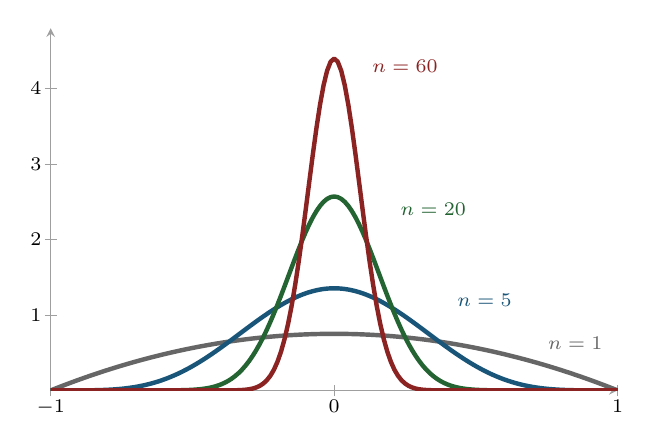
\begin{tikzpicture}
    \begin{axis}[swaxis, width=7.2cm, height=4.6cm, xmin=-1, xmax=1, ymin=0, ymax=4.8,
        xtick={-1,0,1}, ytick={1,2,3,4}, samples=161, domain=-1:1]
      \addplot[gray!80!black, curveln] {0.7500*(1-x^2)^1};
      \addplot[defcolor, curveln] {1.3535*(1-x^2)^5};
      \addplot[proofcolor, curveln] {2.5701*(1-x^2)^20};
      \addplot[thmcolor, curveln] {4.3974*(1-x^2)^60};
      \node[thmcolor, font=\scriptsize, anchor=west] at (axis cs:0.1,4.3) {$n=60$};
      \node[proofcolor, font=\scriptsize, anchor=west] at (axis cs:0.2,2.4) {$n=20$};
      \node[defcolor, font=\scriptsize, anchor=west] at (axis cs:0.4,1.2) {$n=5$};
      \node[gray!80!black, font=\scriptsize, anchor=west] at (axis cs:0.72,0.62) {$n=1$};
    \end{axis}
  \end{tikzpicture}
    \end{column}
  \end{columns}

  \note{
    Rudin remarks that it is instructive to sketch these graphs, so here
    they are. The gray curve is "n" equals 1, the blue one is "n" equals 5,
    the green one is "n" equals 20, and the red one is "n" equals 60. On the
    interval from minus 1 to 1, the base 1 minus "x" squared equals 1 only
    at zero, so a high power crushes everything except a small neighborhood
    of zero. Since the total area stays 1, the peak grows taller as it gets
    narrower. To make this precise, we need to know how large "c" sub "n"
    is.
  }
\end{frame}

% --- Build 1/3 ---
\begin{frame}{Proof of Theorem 7.26 --- How Large Is $c_n$?}
  \begin{hlbox}
  By (48), $\;c_n = 1 \Big/ \displaystyle\int_{-1}^{1} (1-x^2)^n\,dx$: we need a \emph{lower} bound.

  \begin{align*}
    \int_{-1}^{1} (1-x^2)^n\,dx &= 2\int_{0}^{1} (1-x^2)^n\,dx
       \;\ge\; 2\int_{0}^{1/\sqrt{n}} (1-x^2)^n\,dx
  \end{align*}

  \end{hlbox}

  \note{
    By equation 48, the constant "c" sub "n" is the reciprocal of the
    integral of the bump without its constant, that is, of 1 minus "x"
    squared, raised to the power "n". So an upper bound for "c" sub "n"
    requires a lower bound for that integral. The integrand is even, so the
    integral is twice the integral from 0 to 1. Since the integrand is
    nonnegative, we only make things smaller by integrating up to 1 over the
    square root of "n" instead of 1. Why that particular cutoff? Because
    that is roughly the width of the bump, as the next step shows.
  }
\end{frame}

% --- Build 2/3 ---
\begin{frame}{Proof of Theorem 7.26 --- How Large Is $c_n$?}
  \begin{hlbox}
  By (48), $\;c_n = 1 \Big/ \displaystyle\int_{-1}^{1} (1-x^2)^n\,dx$: we need a \emph{lower} bound.

  \begin{align*}
    \int_{-1}^{1} (1-x^2)^n\,dx &= 2\int_{0}^{1} (1-x^2)^n\,dx
       \;\ge\; 2\int_{0}^{1/\sqrt{n}} (1-x^2)^n\,dx
  \\[4pt]
    &\ge 2\int_{0}^{1/\sqrt{n}} (1-nx^2)\,dx
       \;=\; \frac{4}{3\sqrt{n}} \;>\; \frac{1}{\sqrt{n}}
  \end{align*}

  \end{hlbox}

  \note{
    On this short interval we replace the integrand by the simpler
    expression 1 minus "n" times "x" squared, which is smaller. We will
    justify that inequality on the next slide. The new integrand is a
    quadratic that is easy to integrate, and the result is four thirds times
    1 over the square root of "n". Since four thirds is more than 1, that is
    certainly greater than 1 over the square root of "n".
  }
\end{frame}

% --- Build 3/3 ---
\begin{frame}{Proof of Theorem 7.26 --- How Large Is $c_n$?}
  \begin{hlbox}
  By (48), $\;c_n = 1 \Big/ \displaystyle\int_{-1}^{1} (1-x^2)^n\,dx$: we need a \emph{lower} bound.

  \begin{align*}
    \int_{-1}^{1} (1-x^2)^n\,dx &= 2\int_{0}^{1} (1-x^2)^n\,dx
       \;\ge\; 2\int_{0}^{1/\sqrt{n}} (1-x^2)^n\,dx
  \\[4pt]
    &\ge 2\int_{0}^{1/\sqrt{n}} (1-nx^2)\,dx
       \;=\; \frac{4}{3\sqrt{n}} \;>\; \frac{1}{\sqrt{n}}
  \end{align*}
  \vspace{0.3em}
  \begin{center}
    Hence, by (48): \qquad $\boxed{\,c_n < \sqrt{n}\,}$ \hfill (49)
  \end{center}
  \end{hlbox}

  \note{
    So the integral exceeds 1 over the square root of "n", and taking
    reciprocals gives the boxed inequality, equation 49: "c" sub "n" is less
    than the square root of "n". The peak of the kernel grows, but only like
    a square root. That slow growth will be overwhelmed by exponential decay
    away from zero. First, let's settle the inequality we used.
  }
\end{frame}

% --- Build 1/2 ---
\begin{frame}{Why Is $(1-x^2)^n \ge 1 - nx^2$?}
  \begin{columns}[T]
    \begin{column}{0.52\textwidth}
      \begin{proofblock}{Justification}
        Consider, for $0 \le x \le 1$,
        \[
          \varphi(x) = (1-x^2)^n - 1 + nx^2 .
        \]
        \begin{itemize}
          \item $\varphi(0) = 0$
          \item $\varphi'(x) = 2nx\,\bigl[1 - (1-x^2)^{n-1}\bigr] \ge 0$
        \end{itemize}
        So $\varphi \ge 0$ on $[0,1]$.
      \end{proofblock}
    \end{column}
    \begin{column}{0.46\textwidth}
      \centering

    \end{column}
  \end{columns}

  \note{
    Here is the justification. Consider the difference of the two sides, the
    function phi on the slide. At "x" equals 0 it vanishes. Its derivative
    is the product 2 times "n" times "x", multiplied by a bracket, and the
    bracket is 1 minus a number between 0 and 1, so the derivative is
    nonnegative on the unit interval. A function that starts at zero and
    never decreases stays nonnegative, and that is exactly the inequality we
    wanted.
  }
\end{frame}

% --- Build 2/2 ---
\begin{frame}{Why Is $(1-x^2)^n \ge 1 - nx^2$?}
  \begin{columns}[T]
    \begin{column}{0.52\textwidth}
      \begin{proofblock}{Justification}
        Consider, for $0 \le x \le 1$,
        \[
          \varphi(x) = (1-x^2)^n - 1 + nx^2 .
        \]
        \begin{itemize}
          \item $\varphi(0) = 0$
          \item $\varphi'(x) = 2nx\,\bigl[1 - (1-x^2)^{n-1}\bigr] \ge 0$
        \end{itemize}
        So $\varphi \ge 0$ on $[0,1]$.
      \end{proofblock}
    \end{column}
    \begin{column}{0.46\textwidth}
      \centering
  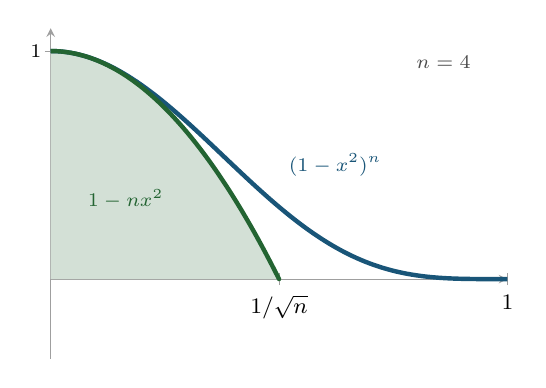
\begin{tikzpicture}
    \begin{axis}[swaxis, width=5.8cm, height=4.2cm, xmin=0, xmax=1, ymin=-0.35, ymax=1.1,
        axis x line=middle, xtick={0.5,1}, xticklabels={$1/\sqrt{n}$,$1$}, ytick={1}, samples=101,
      x tick label style={font=\footnotesize, fill=white, fill opacity=0.6, text opacity=1, inner sep=1.5pt, yshift=-2pt}]
      \addplot[draw=none, fill=proofcolor!20, domain=0:0.5] {1-4*x^2} \closedcycle;
      \addplot[defcolor, curveln, domain=0:1] {(1-x^2)^4};
      \addplot[proofcolor, curveln, domain=0:0.5] {1-4*x^2};
      \node[defcolor, font=\scriptsize, anchor=west] at (axis cs:0.5,0.5) {$(1-x^2)^n$};
      \node[proofcolor, font=\scriptsize, anchor=west] at (axis cs:0.06,0.35) {$1-nx^2$};
      \node[gray!60!black, font=\scriptsize] at (axis cs:0.86,0.95) {$n=4$};
    \end{axis}
  \end{tikzpicture}
    \end{column}
  \end{columns}

  \note{
    The picture on the right shows the case "n" equals 4. The blue curve is
    1 minus "x" squared, raised to the power "n", and the green parabola, 1
    minus "n" times "x" squared, lies below it. The parabola reaches zero
    exactly at 1 over the square root of "n", which explains the cutoff we
    chose. The shaded green region under the parabola, counted twice because
    of the symmetry, gives the lower bound for the integral from the
    previous slide. With the inequality settled, we return to the kernel.
  }
\end{frame}

% --- Build 1/2 ---
\begin{frame}{Proof of Theorem 7.26 --- $Q_n$ Is Small Away from $0$}
  \begin{columns}[T]
    \begin{column}{0.48\textwidth}
      \begin{proofblock}{Tail estimate}
        For any $\delta > 0$, (49) implies
        \[
          Q_n(x) \le \sqrt{n}\,(1-\delta^2)^n \tag{50}
        \]
        for $\delta \le |x| \le 1$.
      \end{proofblock}
    \end{column}
    \begin{column}{0.5\textwidth}
      \centering
  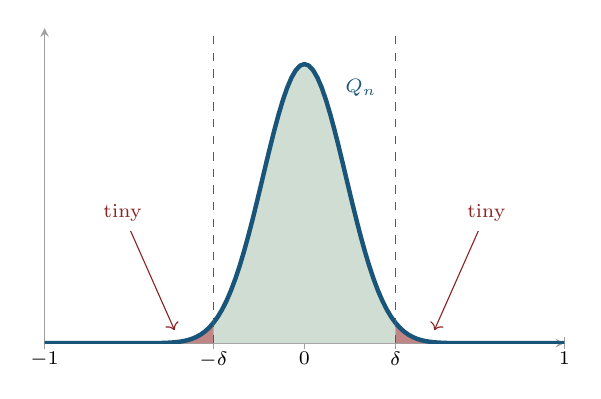
\begin{tikzpicture}
    \begin{axis}[swaxis, width=6.6cm, height=4.0cm, xmin=-1, xmax=1, ymin=0, ymax=2.9,
        xtick={-1,-0.35,0,0.35,1}, xticklabels={$-1$,$-\delta$,$0$,$\delta$,$1$}, ytick=\empty, samples=121]
      \addplot[draw=none, fill=proofcolor!22, domain=-0.35:0.35] {2.5701*(1-x^2)^20} \closedcycle;
      \addplot[draw=none, fill=thmcolor!55, domain=0.35:1] {2.5701*(1-x^2)^20} \closedcycle;
      \addplot[draw=none, fill=thmcolor!55, domain=-1:-0.35] {2.5701*(1-x^2)^20} \closedcycle;
      \addplot[defcolor, curveln, domain=-1:1] {2.5701*(1-x^2)^20};
      \draw[gray!70!black, dashed] (axis cs:-0.35,0) -- (axis cs:-0.35,2.9);
      \draw[gray!70!black, dashed] (axis cs:0.35,0) -- (axis cs:0.35,2.9);
      \node[defcolor, font=\scriptsize, anchor=west] at (axis cs:0.12,2.35) {$Q_n$};
      \node[thmcolor, font=\scriptsize] (tl) at (axis cs:0.7,1.2) {tiny};
      \draw[->, thmcolor] (tl) -- (axis cs:0.5,0.12);
      \node[thmcolor, font=\scriptsize] (tr) at (axis cs:-0.7,1.2) {tiny};
      \draw[->, thmcolor] (tr) -- (axis cs:-0.5,0.12);
    \end{axis}
  \end{tikzpicture}
    \end{column}
  \end{columns}

  \note{
    Now we can quantify the concentration. Fix any positive delta. In the
    picture, the dashed vertical lines mark minus delta and delta. On the
    two outer regions, shaded red, the absolute value of "x" is at least
    delta, so 1 minus "x" squared is at most 1 minus delta squared.
    Combining this with the bound on "c" sub "n" from equation 49 gives
    equation 50: there, capital "Q" sub "n" is at most the square root of
    "n" times the power "n" of 1 minus delta squared.
  }
\end{frame}

% --- Build 2/2 ---
\begin{frame}{Proof of Theorem 7.26 --- $Q_n$ Is Small Away from $0$}
  \begin{columns}[T]
    \begin{column}{0.48\textwidth}
      \begin{proofblock}{Tail estimate}
        For any $\delta > 0$, (49) implies
        \[
          Q_n(x) \le \sqrt{n}\,(1-\delta^2)^n \tag{50}
        \]
        for $\delta \le |x| \le 1$.
      \end{proofblock}

      \vspace{0.5em}
      \begin{hlbox}
      \raggedright
      So $Q_n \to 0$ \alert{uniformly}\\ on $\delta \le |x| \le 1$.

      \smallskip
      {\footnotesize ($\sqrt{n}\,r^n \to 0$ for $0 \le r < 1$;\\ see Theorem 3.20(d).)}
      \end{hlbox}
    \end{column}
    \begin{column}{0.5\textwidth}
      \centering
  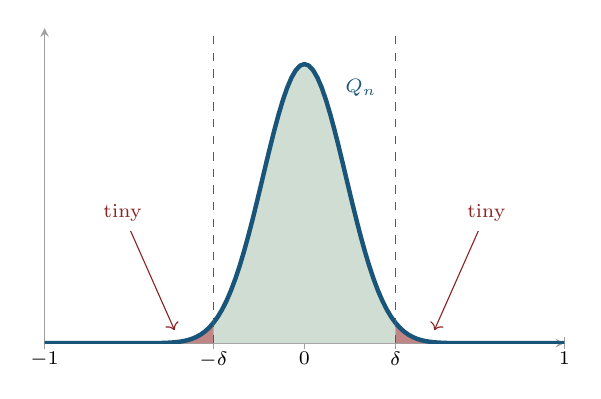
\begin{tikzpicture}
    \begin{axis}[swaxis, width=6.6cm, height=4.0cm, xmin=-1, xmax=1, ymin=0, ymax=2.9,
        xtick={-1,-0.35,0,0.35,1}, xticklabels={$-1$,$-\delta$,$0$,$\delta$,$1$}, ytick=\empty, samples=121]
      \addplot[draw=none, fill=proofcolor!22, domain=-0.35:0.35] {2.5701*(1-x^2)^20} \closedcycle;
      \addplot[draw=none, fill=thmcolor!55, domain=0.35:1] {2.5701*(1-x^2)^20} \closedcycle;
      \addplot[draw=none, fill=thmcolor!55, domain=-1:-0.35] {2.5701*(1-x^2)^20} \closedcycle;
      \addplot[defcolor, curveln, domain=-1:1] {2.5701*(1-x^2)^20};
      \draw[gray!70!black, dashed] (axis cs:-0.35,0) -- (axis cs:-0.35,2.9);
      \draw[gray!70!black, dashed] (axis cs:0.35,0) -- (axis cs:0.35,2.9);
      \node[defcolor, font=\scriptsize, anchor=west] at (axis cs:0.12,2.35) {$Q_n$};
      \node[thmcolor, font=\scriptsize] (tl) at (axis cs:0.7,1.2) {tiny};
      \draw[->, thmcolor] (tl) -- (axis cs:0.5,0.12);
      \node[thmcolor, font=\scriptsize] (tr) at (axis cs:-0.7,1.2) {tiny};
      \draw[->, thmcolor] (tr) -- (axis cs:-0.5,0.12);
    \end{axis}
  \end{tikzpicture}
    \end{column}
  \end{columns}

  \note{
    The right side of equation 50 does not depend on "x", and it tends to
    zero as "n" goes to infinity. Indeed, 1 minus delta squared is a fixed
    number below 1, so its powers decay exponentially, and exponential decay
    beats the growth of the square root. That is part "d" of Theorem 3.20.
    Hence the kernels converge to zero uniformly on the red regions. Since
    the total area is always 1, almost all of it must sit in the green
    region between minus delta and delta. Now we are ready to define the
    approximating polynomials.
  }
\end{frame}

% --- Build 1/2 ---
\begin{frame}{Proof of Theorem 7.26 --- The Polynomials $P_n$}
  \begin{proofblock}{Definition of $P_n$}
    \[
      P_n(x) = \int_{-1}^{1} f(x+t)\,Q_n(t)\,dt \qquad (0 \le x \le 1). \tag{51}
    \]
  \end{proofblock}

  \note{
    Equation 51 defines capital "P" sub "n". For each "x" in the unit
    interval, we integrate the values of "f" at the shifted points "x" plus
    "t" against the kernel capital "Q" sub "n" of "t", for "t" from minus 1
    to 1. Remember that "f" has been extended by zero, so evaluating "f" at
    "x" plus "t" makes sense even when that point leaves the unit interval.
    Since the kernel is nonnegative and has total integral 1, this is a
    weighted average of values of "f".
  }
\end{frame}

% --- Build 2/2 ---
\begin{frame}{Proof of Theorem 7.26 --- The Polynomials $P_n$}
  \begin{proofblock}{Definition of $P_n$}
    \[
      P_n(x) = \int_{-1}^{1} f(x+t)\,Q_n(t)\,dt \qquad (0 \le x \le 1). \tag{51}
    \]
  \end{proofblock}
  \vspace{0.3em}
  \begin{center}
  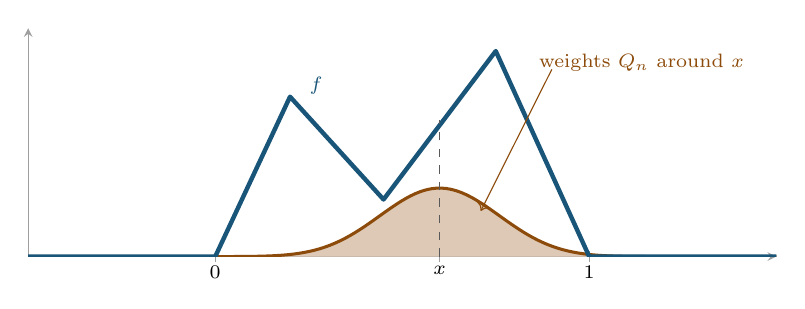
\begin{tikzpicture}
    \begin{axis}[swaxis, width=9.5cm, height=2.9cm, xmin=-0.5, xmax=1.5, ymin=0, ymax=1.0,
        xtick={0,0.6,1}, xticklabels={$0$,$x$,$1$}, ytick=\empty, samples=141]
      \addplot[draw=none, fill=excolor!30, domain=-0.4:1.5] {0.3*(1-(x-0.6)^2)^20} \closedcycle;
      \addplot[excolor, line width=1.1pt, domain=-0.4:1.5] {0.3*(1-(x-0.6)^2)^20};
      \addplot[defcolor, curveln] coordinates {(-0.5,0) (0,0) (0.2,0.7) (0.45,0.25) (0.75,0.9) (1,0) (1.5,0)};
      \draw[gray!70!black, dashed] (axis cs:0.6,0) -- (axis cs:0.6,0.6);
      \node[defcolor, font=\scriptsize] at (axis cs:0.27,0.75) {$f$};
      \node[excolor, font=\scriptsize, anchor=west] at (axis cs:0.84,0.85) {weights $Q_n$ around $x$};
      \draw[->, excolor] (axis cs:0.9,0.82) -- (axis cs:0.71,0.2);
    \end{axis}
  \end{tikzpicture}

  \smallskip
  \hl{$P_n(x)$ is a \alert{weighted average} of the values of $f$ near $x$.}
  \end{center}

  \note{
    The picture shows what is being averaged. The blue graph is "f",
    extended by zero outside the unit interval. The amber bump is the
    kernel, shifted so that it is centered at the point "x". Values of "f"
    close to "x" receive almost all the weight, and values far away receive
    almost none. As "n" grows the bump narrows, so the average should
    approach "f" of "x" itself. But first, why is capital "P" sub "n" a
    polynomial?
  }
\end{frame}

% --- Build 1/3 ---
\begin{frame}{Proof of Theorem 7.26 --- $P_n$ Is a Polynomial}
  \begin{proofblock}{Change of variable}
    Since $f = 0$ outside $[0,1]$, only $-x \le t \le 1-x$ contributes:
    \[
      P_n(x) = \int_{-x}^{1-x} f(x+t)\,Q_n(t)\,dt
  \]
  \end{proofblock}

  \note{
    Recall that "f" vanishes outside the unit interval. So the integrand in
    equation 51 is zero unless "x" plus "t" lies between 0 and 1, that is,
    unless "t" lies between minus "x" and 1 minus "x". Since "x" is in the
    unit interval, this range is contained in the interval from minus 1 to
    1. So we may shrink the limits of integration, as shown.
  }
\end{frame}

% --- Build 2/3 ---
\begin{frame}{Proof of Theorem 7.26 --- $P_n$ Is a Polynomial}
  \begin{proofblock}{Change of variable}
    Since $f = 0$ outside $[0,1]$, only $-x \le t \le 1-x$ contributes:
    \[
      P_n(x) = \int_{-x}^{1-x} f(x+t)\,Q_n(t)\,dt
             = \int_{0}^{1} f(t)\,Q_n(t-x)\,dt .
  \]
  \end{proofblock}

  \note{
    Now substitute a new variable for "x" plus "t". Following the book, we
    call the new variable "t" again. The limits become 0 and 1, the function
    "f" is evaluated at "t", and the kernel is evaluated at "t" minus "x".
    The variable "x" has moved out of "f" and into the kernel. That is the
    whole point of the substitution.
  }
\end{frame}

% --- Build 3/3 ---
\begin{frame}{Proof of Theorem 7.26 --- $P_n$ Is a Polynomial}
  \begin{proofblock}{Change of variable}
    Since $f = 0$ outside $[0,1]$, only $-x \le t \le 1-x$ contributes:
    \[
      P_n(x) = \int_{-x}^{1-x} f(x+t)\,Q_n(t)\,dt
             = \int_{0}^{1} f(t)\,Q_n(t-x)\,dt .
  \]
  \end{proofblock}
  \vspace{0.5em}
  \begin{hlbox}
  $Q_n(t-x) = c_n\,[1 - (t-x)^2]^n$ is a polynomial in $x$ whose coefficients depend on $t$.

  \smallskip
  $\Longrightarrow\;$ $P_n$ is a \alert{polynomial} in $x$ (of degree at most $2n$), real if $f$ is real.
  \end{hlbox}

  \note{
    Why does this help? Expand the kernel in powers of "x". It is a
    polynomial in "x" of degree 2 times "n" whose coefficients are
    polynomials in "t". Multiply by "f" of "t" and integrate over "t" from 0
    to 1. Each coefficient integrates to a number, so the result is a
    polynomial in "x" of degree at most 2 times "n". If "f" is real, those
    numbers are real. So we have a sequence of polynomials, and it remains
    to show that it converges to "f" uniformly.
  }
\end{frame}

% --- Build 1/3 ---
\begin{frame}{Proof of Theorem 7.26 --- Setting Up the Estimate}
  \begin{proofblock}{Ingredients}
    \begin{enumerate}\setlength{\itemsep}{0.4em}
      \item Given $\varepsilon > 0$, choose $\delta > 0$ such that
        \[
          |y - x| < \delta \;\Longrightarrow\; |f(y) - f(x)| < \frac{\varepsilon}{2} .
        \]
    \end{enumerate}
  \end{proofblock}

  \note{
    We collect three ingredients. First, let epsilon be given. Because "f"
    is uniformly continuous on the whole line, there is a delta such that
    any two points closer than delta have function values closer than
    epsilon over 2. The crucial feature is that one delta works for every
    point "x". This is where extending "f" by zero to the whole line pays
    off.
  }
\end{frame}

% --- Build 2/3 ---
\begin{frame}{Proof of Theorem 7.26 --- Setting Up the Estimate}
  \begin{proofblock}{Ingredients}
    \begin{enumerate}\setlength{\itemsep}{0.4em}
      \item Given $\varepsilon > 0$, choose $\delta > 0$ such that
        \[
          |y - x| < \delta \;\Longrightarrow\; |f(y) - f(x)| < \frac{\varepsilon}{2} .
        \]
      \item Let $M = \sup |f(x)|$. Then $|f(x+t) - f(x)| \le 2M$ for all $x$, $t$.
    \end{enumerate}
  \end{proofblock}

  \note{
    Second, let capital "M" be the supremum of the absolute value of "f". It
    is finite because "f" is continuous on a compact interval and zero
    elsewhere. Then the difference of any two values of "f" is at most 2
    times capital "M" in absolute value. This is a crude bound, but we will
    only use it where the kernel is tiny.
  }
\end{frame}

% --- Build 3/3 ---
\begin{frame}{Proof of Theorem 7.26 --- Setting Up the Estimate}
  \begin{proofblock}{Ingredients}
    \begin{enumerate}\setlength{\itemsep}{0.4em}
      \item Given $\varepsilon > 0$, choose $\delta > 0$ such that
        \[
          |y - x| < \delta \;\Longrightarrow\; |f(y) - f(x)| < \frac{\varepsilon}{2} .
        \]
      \item Let $M = \sup |f(x)|$. Then $|f(x+t) - f(x)| \le 2M$ for all $x$, $t$.
      \item By (48), $f(x) = \displaystyle\int_{-1}^{1} f(x)\,Q_n(t)\,dt$, hence
        \[
          P_n(x) - f(x) = \int_{-1}^{1} \bigl[f(x+t) - f(x)\bigr]\,Q_n(t)\,dt .
        \]
    \end{enumerate}
  \end{proofblock}

  \note{
    Third, a small trick. Since the kernel has integral 1 by equation 48,
    the number "f" of "x" equals the integral of "f" of "x" times the
    kernel. Here "f" of "x" does not depend on "t", so it is a constant
    inside the integral. Subtracting this from equation 51, the error
    capital "P" sub "n" of "x" minus "f" of "x" becomes a single integral.
    Its integrand is the change in "f" between the point "x" and the shifted
    point "x" plus "t", weighted by the kernel. Now we estimate this
    integral.
  }
\end{frame}

% --- Build 1/4 ---
\begin{frame}{Proof of Theorem 7.26 --- The Estimate}
  \begin{hlbox}
  For $0 \le x \le 1$:
  {\small
  \begin{align*}
    |P_n(x) - f(x)|
      &= \left| \int_{-1}^{1} [f(x+t) - f(x)]\,Q_n(t)\,dt \right|
       \;\le\; \int_{-1}^{1} |f(x+t) - f(x)|\,Q_n(t)\,dt
  \end{align*}}

  \end{hlbox}

  \note{
    Take any "x" in the unit interval. The absolute value of the error is
    the absolute value of the integral from the previous slide. We move the
    absolute value inside the integral. Because the kernel is nonnegative,
    it needs no absolute value of its own. This is one of the places where
    positivity of capital "Q" sub "n" is used.
  }
\end{frame}

% --- Build 2/4 ---
\begin{frame}{Proof of Theorem 7.26 --- The Estimate}
  \begin{hlbox}
  For $0 \le x \le 1$:
  {\small
  \begin{align*}
    |P_n(x) - f(x)|
      &= \left| \int_{-1}^{1} [f(x+t) - f(x)]\,Q_n(t)\,dt \right|
       \;\le\; \int_{-1}^{1} |f(x+t) - f(x)|\,Q_n(t)\,dt
  \\[3pt]
      &\le 2M \int_{-1}^{-\delta} Q_n(t)\,dt
         + \frac{\varepsilon}{2} \int_{-\delta}^{\delta} Q_n(t)\,dt
         + 2M \int_{\delta}^{1} Q_n(t)\,dt
  \end{align*}}

  \end{hlbox}

  \note{
    Now split the range of integration into three pieces. In the middle
    piece, "t" lies between minus delta and delta, so by the choice of delta
    the difference of the values of "f" is less than epsilon over 2. In the
    two outer pieces we use the crude bound 2 times capital "M". This gives
    the three integrals on the slide.
  }
\end{frame}

% --- Build 3/4 ---
\begin{frame}{Proof of Theorem 7.26 --- The Estimate}
  \begin{hlbox}
  For $0 \le x \le 1$:
  {\small
  \begin{align*}
    |P_n(x) - f(x)|
      &= \left| \int_{-1}^{1} [f(x+t) - f(x)]\,Q_n(t)\,dt \right|
       \;\le\; \int_{-1}^{1} |f(x+t) - f(x)|\,Q_n(t)\,dt
  \\[3pt]
      &\le 2M \int_{-1}^{-\delta} Q_n(t)\,dt
         + \frac{\varepsilon}{2} \int_{-\delta}^{\delta} Q_n(t)\,dt
         + 2M \int_{\delta}^{1} Q_n(t)\,dt
  \\[3pt]
      &\le 4M\sqrt{n}\,(1-\delta^2)^n + \frac{\varepsilon}{2}
  \end{align*}}

  \end{hlbox}

  \note{
    For the middle integral, the kernel integrates to at most 1, by equation
    48, so that term is at most epsilon over 2. For the outer integrals we
    use the tail estimate, equation 50. Each outer interval has length less
    than 1, and on it the kernel is at most the square root of "n" times the
    power "n" of 1 minus delta squared. Two such pieces, each with the
    factor 2 times capital "M", give the first term on the slide.
  }
\end{frame}

% --- Build 4/4 ---
\begin{frame}{Proof of Theorem 7.26 --- The Estimate}
  \begin{hlbox}
  For $0 \le x \le 1$:
  {\small
  \begin{align*}
    |P_n(x) - f(x)|
      &= \left| \int_{-1}^{1} [f(x+t) - f(x)]\,Q_n(t)\,dt \right|
       \;\le\; \int_{-1}^{1} |f(x+t) - f(x)|\,Q_n(t)\,dt
  \\[3pt]
      &\le 2M \int_{-1}^{-\delta} Q_n(t)\,dt
         + \frac{\varepsilon}{2} \int_{-\delta}^{\delta} Q_n(t)\,dt
         + 2M \int_{\delta}^{1} Q_n(t)\,dt
  \\[3pt]
      &\le 4M\sqrt{n}\,(1-\delta^2)^n + \frac{\varepsilon}{2}
  \\[3pt]
      &< \varepsilon \qquad \text{for all large enough } n .
  \end{align*}}
  \vspace{0.2em}
  The bound does not depend on $x$ $\;\Longrightarrow\;$ $P_n \to f$ \alert{uniformly} on $[0,1]$.
  \hfill $\blacksquare$
  \end{hlbox}

  \note{
    Finally, as we saw, the first term tends to zero as "n" grows, so it is
    eventually below epsilon over 2, and the total is less than epsilon. The
    key observation is that nothing in the final bound depends on "x". One
    threshold for "n" works for every point of the unit interval. So the
    polynomials converge to "f" uniformly, and the Weierstrass theorem is
    proved.
  }
\end{frame}

% --- Build 1/2 ---
\begin{frame}{Theorem 7.26 in Action}
  \begin{columns}[T]
    \begin{column}{0.56\textwidth}
      \centering
  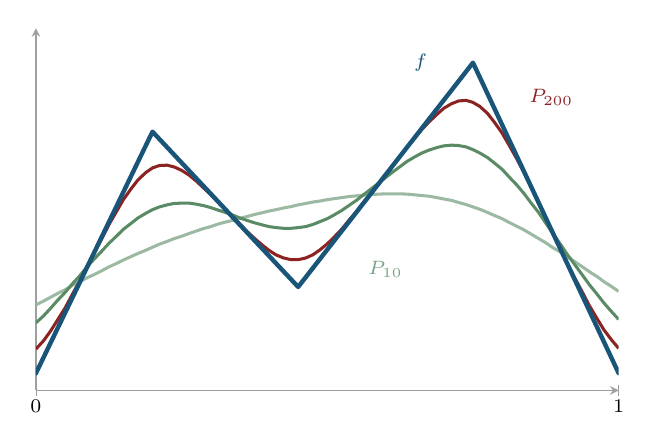
\begin{tikzpicture}
    \begin{axis}[swaxis, width=7.4cm, height=4.6cm, xmin=0, xmax=1, ymin=-0.05, ymax=1.0,
        xtick={0,1}, ytick=\empty]
      \addplot[proofcolor!45, line width=1.1pt] coordinates {(0.000,0.198) (0.013,0.209) (0.025,0.220) (0.037,0.231) (0.050,0.242) (0.062,0.254) (0.075,0.265) (0.087,0.276) (0.100,0.286) (0.113,0.297) (0.125,0.308) (0.138,0.318) (0.150,0.328) (0.163,0.338) (0.175,0.347) (0.188,0.356) (0.200,0.365) (0.212,0.374) (0.225,0.382) (0.237,0.390) (0.250,0.397) (0.263,0.405) (0.275,0.412) (0.287,0.419) (0.300,0.425) (0.312,0.432) (0.325,0.438) (0.338,0.443) (0.350,0.449) (0.362,0.454) (0.375,0.460) (0.388,0.465) (0.400,0.470) (0.412,0.474) (0.425,0.479) (0.438,0.483) (0.450,0.488) (0.463,0.492) (0.475,0.496) (0.487,0.499) (0.500,0.503) (0.512,0.506) (0.525,0.509) (0.537,0.512) (0.550,0.514) (0.562,0.516) (0.575,0.518) (0.588,0.519) (0.600,0.520) (0.613,0.520) (0.625,0.520) (0.637,0.519) (0.650,0.517) (0.662,0.515) (0.675,0.513) (0.688,0.509) (0.700,0.505) (0.713,0.501) (0.725,0.495) (0.738,0.489) (0.750,0.482) (0.762,0.475) (0.775,0.466) (0.787,0.457) (0.800,0.448) (0.812,0.437) (0.825,0.426) (0.838,0.415) (0.850,0.403) (0.863,0.390) (0.875,0.378) (0.887,0.364) (0.900,0.351) (0.912,0.337) (0.925,0.323) (0.938,0.308) (0.950,0.294) (0.963,0.280) (0.975,0.265) (0.988,0.251) (1.000,0.237)};
      \addplot[proofcolor!75, line width=1.1pt] coordinates {(0.000,0.146) (0.013,0.166) (0.025,0.188) (0.037,0.211) (0.050,0.234) (0.062,0.258) (0.075,0.282) (0.087,0.307) (0.100,0.331) (0.113,0.354) (0.125,0.376) (0.138,0.397) (0.150,0.417) (0.163,0.434) (0.175,0.450) (0.188,0.463) (0.200,0.474) (0.212,0.482) (0.225,0.488) (0.237,0.492) (0.250,0.493) (0.263,0.493) (0.275,0.490) (0.287,0.486) (0.300,0.480) (0.312,0.473) (0.325,0.466) (0.338,0.458) (0.350,0.450) (0.362,0.443) (0.375,0.436) (0.388,0.430) (0.400,0.425) (0.412,0.422) (0.425,0.420) (0.438,0.420) (0.450,0.422) (0.463,0.425) (0.475,0.431) (0.487,0.439) (0.500,0.448) (0.512,0.459) (0.525,0.472) (0.537,0.486) (0.550,0.501) (0.562,0.517) (0.575,0.534) (0.588,0.551) (0.600,0.567) (0.613,0.584) (0.625,0.599) (0.637,0.614) (0.650,0.627) (0.662,0.638) (0.675,0.647) (0.688,0.654) (0.700,0.659) (0.713,0.661) (0.725,0.660) (0.738,0.656) (0.750,0.648) (0.762,0.638) (0.775,0.625) (0.787,0.609) (0.800,0.591) (0.812,0.569) (0.825,0.546) (0.838,0.520) (0.850,0.493) (0.863,0.465) (0.875,0.435) (0.887,0.405) (0.900,0.374) (0.912,0.344) (0.925,0.314) (0.938,0.284) (0.950,0.256) (0.963,0.229) (0.975,0.203) (0.988,0.178) (1.000,0.156)};
      \addplot[thmcolor, line width=1.1pt] coordinates {(0.000,0.070) (0.013,0.094) (0.025,0.122) (0.037,0.154) (0.050,0.189) (0.062,0.227) (0.075,0.267) (0.087,0.308) (0.100,0.349) (0.113,0.390) (0.125,0.430) (0.138,0.468) (0.150,0.503) (0.163,0.534) (0.175,0.560) (0.188,0.581) (0.200,0.595) (0.212,0.602) (0.225,0.603) (0.237,0.598) (0.250,0.588) (0.263,0.574) (0.275,0.557) (0.287,0.538) (0.300,0.518) (0.312,0.497) (0.325,0.475) (0.338,0.453) (0.350,0.432) (0.362,0.411) (0.375,0.391) (0.388,0.372) (0.400,0.356) (0.412,0.343) (0.425,0.334) (0.438,0.329) (0.450,0.329) (0.463,0.334) (0.475,0.343) (0.487,0.357) (0.500,0.375) (0.512,0.395) (0.525,0.418) (0.537,0.443) (0.550,0.468) (0.562,0.495) (0.575,0.521) (0.588,0.548) (0.600,0.575) (0.613,0.602) (0.625,0.629) (0.637,0.655) (0.650,0.681) (0.662,0.706) (0.675,0.729) (0.688,0.750) (0.700,0.768) (0.713,0.781) (0.725,0.789) (0.738,0.791) (0.750,0.785) (0.762,0.773) (0.775,0.753) (0.787,0.727) (0.800,0.696) (0.812,0.661) (0.825,0.622) (0.838,0.580) (0.850,0.538) (0.863,0.494) (0.875,0.450) (0.887,0.405) (0.900,0.361) (0.912,0.318) (0.925,0.275) (0.938,0.234) (0.950,0.195) (0.963,0.158) (0.975,0.125) (0.988,0.096) (1.000,0.072)};
      \addplot[defcolor, curveln] coordinates {(0,0) (0.2,0.7) (0.45,0.25) (0.75,0.9) (1,0)};
      \node[defcolor, font=\scriptsize] at (axis cs:0.66,0.9) {$f$};
      \node[proofcolor!60, font=\scriptsize] at (axis cs:0.6,0.3) {$P_{10}$};
      \node[thmcolor, font=\scriptsize, anchor=west] at (axis cs:0.83,0.8) {$P_{200}$};
    \end{axis}
  \end{tikzpicture}
    \end{column}
    \begin{column}{0.42\textwidth}
      \centering

    \end{column}
  \end{columns}

  \note{
    Let's see the construction at work. The blue zigzag is a continuous
    function on the unit interval that vanishes at both endpoints. The other
    three curves are the polynomials from the proof. The light green one is
    capital "P" sub 10, the darker green one is capital "P" sub 40, and the
    red one is capital "P" sub 200. Each is a smoothed version of "f", and
    they close in on the zigzag, most slowly at the corners.
  }
\end{frame}

% --- Build 2/2 ---
\begin{frame}{Theorem 7.26 in Action}
  \begin{columns}[T]
    \begin{column}{0.56\textwidth}
      \centering
  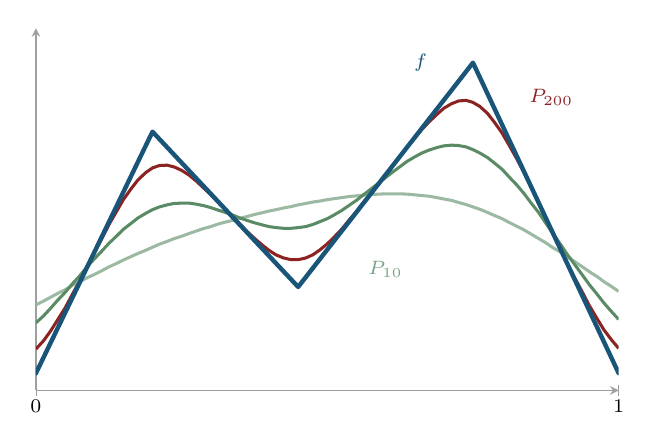
\begin{tikzpicture}
    \begin{axis}[swaxis, width=7.4cm, height=4.6cm, xmin=0, xmax=1, ymin=-0.05, ymax=1.0,
        xtick={0,1}, ytick=\empty]
      \addplot[proofcolor!45, line width=1.1pt] coordinates {(0.000,0.198) (0.013,0.209) (0.025,0.220) (0.037,0.231) (0.050,0.242) (0.062,0.254) (0.075,0.265) (0.087,0.276) (0.100,0.286) (0.113,0.297) (0.125,0.308) (0.138,0.318) (0.150,0.328) (0.163,0.338) (0.175,0.347) (0.188,0.356) (0.200,0.365) (0.212,0.374) (0.225,0.382) (0.237,0.390) (0.250,0.397) (0.263,0.405) (0.275,0.412) (0.287,0.419) (0.300,0.425) (0.312,0.432) (0.325,0.438) (0.338,0.443) (0.350,0.449) (0.362,0.454) (0.375,0.460) (0.388,0.465) (0.400,0.470) (0.412,0.474) (0.425,0.479) (0.438,0.483) (0.450,0.488) (0.463,0.492) (0.475,0.496) (0.487,0.499) (0.500,0.503) (0.512,0.506) (0.525,0.509) (0.537,0.512) (0.550,0.514) (0.562,0.516) (0.575,0.518) (0.588,0.519) (0.600,0.520) (0.613,0.520) (0.625,0.520) (0.637,0.519) (0.650,0.517) (0.662,0.515) (0.675,0.513) (0.688,0.509) (0.700,0.505) (0.713,0.501) (0.725,0.495) (0.738,0.489) (0.750,0.482) (0.762,0.475) (0.775,0.466) (0.787,0.457) (0.800,0.448) (0.812,0.437) (0.825,0.426) (0.838,0.415) (0.850,0.403) (0.863,0.390) (0.875,0.378) (0.887,0.364) (0.900,0.351) (0.912,0.337) (0.925,0.323) (0.938,0.308) (0.950,0.294) (0.963,0.280) (0.975,0.265) (0.988,0.251) (1.000,0.237)};
      \addplot[proofcolor!75, line width=1.1pt] coordinates {(0.000,0.146) (0.013,0.166) (0.025,0.188) (0.037,0.211) (0.050,0.234) (0.062,0.258) (0.075,0.282) (0.087,0.307) (0.100,0.331) (0.113,0.354) (0.125,0.376) (0.138,0.397) (0.150,0.417) (0.163,0.434) (0.175,0.450) (0.188,0.463) (0.200,0.474) (0.212,0.482) (0.225,0.488) (0.237,0.492) (0.250,0.493) (0.263,0.493) (0.275,0.490) (0.287,0.486) (0.300,0.480) (0.312,0.473) (0.325,0.466) (0.338,0.458) (0.350,0.450) (0.362,0.443) (0.375,0.436) (0.388,0.430) (0.400,0.425) (0.412,0.422) (0.425,0.420) (0.438,0.420) (0.450,0.422) (0.463,0.425) (0.475,0.431) (0.487,0.439) (0.500,0.448) (0.512,0.459) (0.525,0.472) (0.537,0.486) (0.550,0.501) (0.562,0.517) (0.575,0.534) (0.588,0.551) (0.600,0.567) (0.613,0.584) (0.625,0.599) (0.637,0.614) (0.650,0.627) (0.662,0.638) (0.675,0.647) (0.688,0.654) (0.700,0.659) (0.713,0.661) (0.725,0.660) (0.738,0.656) (0.750,0.648) (0.762,0.638) (0.775,0.625) (0.787,0.609) (0.800,0.591) (0.812,0.569) (0.825,0.546) (0.838,0.520) (0.850,0.493) (0.863,0.465) (0.875,0.435) (0.887,0.405) (0.900,0.374) (0.912,0.344) (0.925,0.314) (0.938,0.284) (0.950,0.256) (0.963,0.229) (0.975,0.203) (0.988,0.178) (1.000,0.156)};
      \addplot[thmcolor, line width=1.1pt] coordinates {(0.000,0.070) (0.013,0.094) (0.025,0.122) (0.037,0.154) (0.050,0.189) (0.062,0.227) (0.075,0.267) (0.087,0.308) (0.100,0.349) (0.113,0.390) (0.125,0.430) (0.138,0.468) (0.150,0.503) (0.163,0.534) (0.175,0.560) (0.188,0.581) (0.200,0.595) (0.212,0.602) (0.225,0.603) (0.237,0.598) (0.250,0.588) (0.263,0.574) (0.275,0.557) (0.287,0.538) (0.300,0.518) (0.312,0.497) (0.325,0.475) (0.338,0.453) (0.350,0.432) (0.362,0.411) (0.375,0.391) (0.388,0.372) (0.400,0.356) (0.412,0.343) (0.425,0.334) (0.438,0.329) (0.450,0.329) (0.463,0.334) (0.475,0.343) (0.487,0.357) (0.500,0.375) (0.512,0.395) (0.525,0.418) (0.537,0.443) (0.550,0.468) (0.562,0.495) (0.575,0.521) (0.588,0.548) (0.600,0.575) (0.613,0.602) (0.625,0.629) (0.637,0.655) (0.650,0.681) (0.662,0.706) (0.675,0.729) (0.688,0.750) (0.700,0.768) (0.713,0.781) (0.725,0.789) (0.738,0.791) (0.750,0.785) (0.762,0.773) (0.775,0.753) (0.787,0.727) (0.800,0.696) (0.812,0.661) (0.825,0.622) (0.838,0.580) (0.850,0.538) (0.863,0.494) (0.875,0.450) (0.887,0.405) (0.900,0.361) (0.912,0.318) (0.925,0.275) (0.938,0.234) (0.950,0.195) (0.963,0.158) (0.975,0.125) (0.988,0.096) (1.000,0.072)};
      \addplot[defcolor, curveln] coordinates {(0,0) (0.2,0.7) (0.45,0.25) (0.75,0.9) (1,0)};
      \node[defcolor, font=\scriptsize] at (axis cs:0.66,0.9) {$f$};
      \node[proofcolor!60, font=\scriptsize] at (axis cs:0.6,0.3) {$P_{10}$};
      \node[thmcolor, font=\scriptsize, anchor=west] at (axis cs:0.83,0.8) {$P_{200}$};
    \end{axis}
  \end{tikzpicture}
    \end{column}
    \begin{column}{0.42\textwidth}
      \centering
      \vspace{1em}
      \begin{remblock}{Remarks}
        \raggedright
        \begin{itemize}
          \item It is instructive to sketch the graphs of $Q_n$ for a few values of $n$.
          \item We needed uniform \emph{continuity} of $f$ to deduce uniform
            \emph{convergence} of $\{P_n\}$.
        \end{itemize}
      \end{remblock}
    \end{column}
  \end{columns}

  \note{
    On the right are two remarks from the book. The first is the advice to
    sketch the kernels, which we followed earlier. The second is a point
    about the logic. We needed a single delta that works at every point, in
    other words uniform continuity, precisely in order to get convergence
    that is uniform. Next, we look at a special case that will be essential
    later.
  }
\end{frame}
}

{
\usebackgroundtemplate{%
  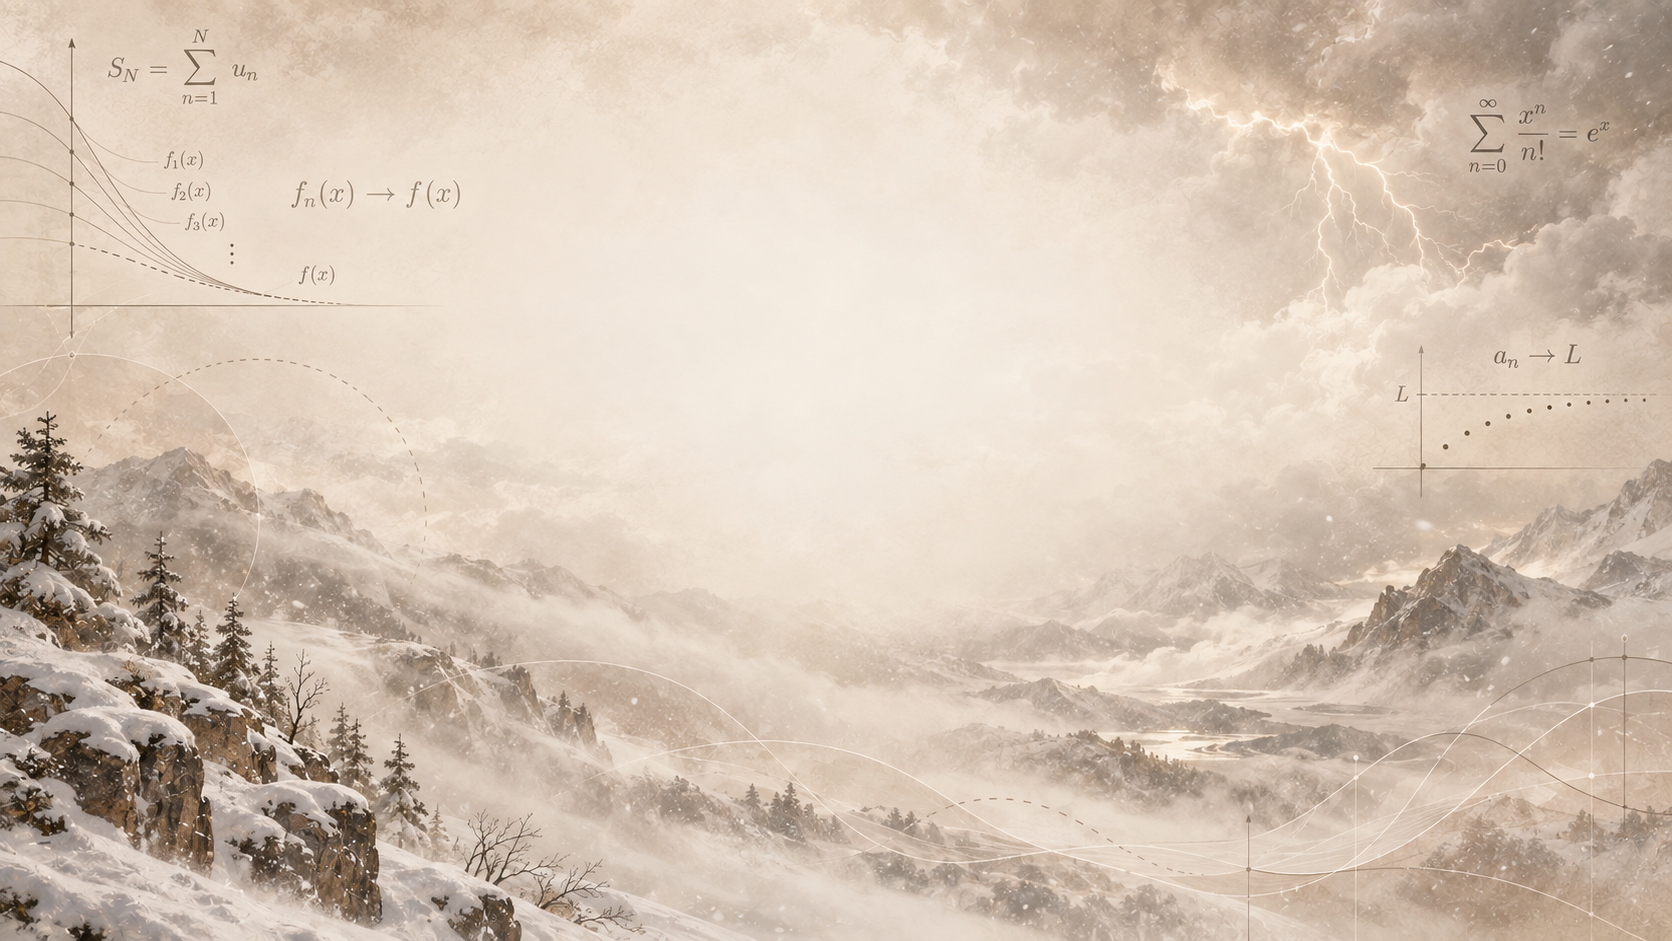
\includegraphics[width=\paperwidth,height=\paperheight,keepaspectratio=false]{chapter_07_bg_04.png}%
}
\section{The Absolute Value}

% --- Build 1/2 ---
\begin{frame}{Corollary 7.27: Approximating $|x|$}
  \begin{thmblock}{Corollary 7.27}
    For every interval $[-a, a]$ there is a sequence of real polynomials $P_n$ such that
    $P_n(0) = 0$ and such that
    \[
      \lim_{n \to \infty} P_n(x) = |x|
    \]
    uniformly on $[-a, a]$.
  \end{thmblock}

  \note{
    In the proof of Stone's theorem we will not need the full strength of
    the Weierstrass theorem. We only need one special case, which Rudin
    states as Corollary 7.27. On any symmetric interval from minus "a" to
    "a", the absolute value function is a uniform limit of real polynomials.
    Moreover, these polynomials can be chosen to vanish at zero. The
    absolute value is the simplest continuous function with a corner, so
    this is a genuine test of the theorem.
  }
\end{frame}

% --- Build 2/2 ---
\begin{frame}{Corollary 7.27: Approximating $|x|$}
  \begin{thmblock}{Corollary 7.27}
    For every interval $[-a, a]$ there is a sequence of real polynomials $P_n$ such that
    $P_n(0) = 0$ and such that
    \[
      \lim_{n \to \infty} P_n(x) = |x|
    \]
    uniformly on $[-a, a]$.
  \end{thmblock}
  \vspace{0.3em}
  \begin{columns}[c]
    \begin{column}{0.52\textwidth}
      \centering
  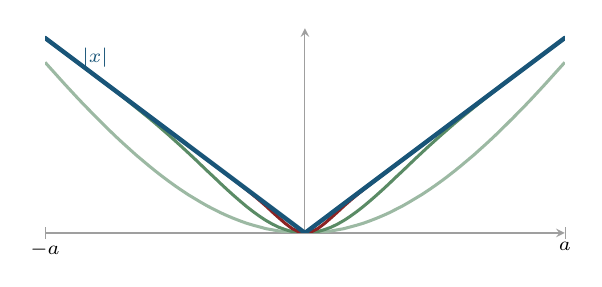
\begin{tikzpicture}
    \begin{axis}[swaxis, width=6.6cm, height=2.6cm, xmin=-1, xmax=1, ymin=0, ymax=1.05,
        axis y line=middle, xtick={-1,1}, xticklabels={$-a$,$a$}, ytick=\empty]
      \addplot[proofcolor!45, line width=1.1pt] coordinates {(-1.000,0.875) (-0.975,0.838) (-0.950,0.801) (-0.925,0.764) (-0.900,0.728) (-0.875,0.692) (-0.850,0.657) (-0.825,0.623) (-0.800,0.589) (-0.775,0.556) (-0.750,0.523) (-0.725,0.491) (-0.700,0.460) (-0.675,0.430) (-0.650,0.400) (-0.625,0.372) (-0.600,0.344) (-0.575,0.317) (-0.550,0.291) (-0.525,0.266) (-0.500,0.242) (-0.475,0.219) (-0.450,0.197) (-0.425,0.177) (-0.400,0.157) (-0.375,0.138) (-0.350,0.121) (-0.325,0.104) (-0.300,0.089) (-0.275,0.075) (-0.250,0.062) (-0.225,0.050) (-0.200,0.040) (-0.175,0.031) (-0.150,0.022) (-0.125,0.016) (-0.100,0.010) (-0.075,0.006) (-0.050,0.002) (-0.025,0.001) (0.000,0.000) (0.025,0.001) (0.050,0.002) (0.075,0.006) (0.100,0.010) (0.125,0.016) (0.150,0.022) (0.175,0.031) (0.200,0.040) (0.225,0.050) (0.250,0.062) (0.275,0.075) (0.300,0.089) (0.325,0.104) (0.350,0.121) (0.375,0.138) (0.400,0.157) (0.425,0.177) (0.450,0.197) (0.475,0.219) (0.500,0.242) (0.525,0.266) (0.550,0.291) (0.575,0.317) (0.600,0.344) (0.625,0.372) (0.650,0.400) (0.675,0.430) (0.700,0.460) (0.725,0.491) (0.750,0.523) (0.775,0.556) (0.800,0.589) (0.825,0.623) (0.850,0.657) (0.875,0.692) (0.900,0.728) (0.925,0.764) (0.950,0.801) (0.975,0.838) (1.000,0.875)};
      \addplot[proofcolor!75, line width=1.1pt] coordinates {(-1.000,1.000) (-0.975,0.975) (-0.950,0.950) (-0.925,0.925) (-0.900,0.900) (-0.875,0.875) (-0.850,0.850) (-0.825,0.825) (-0.800,0.799) (-0.775,0.774) (-0.750,0.748) (-0.725,0.723) (-0.700,0.697) (-0.675,0.670) (-0.650,0.643) (-0.625,0.616) (-0.600,0.589) (-0.575,0.561) (-0.550,0.532) (-0.525,0.503) (-0.500,0.473) (-0.475,0.443) (-0.450,0.412) (-0.425,0.381) (-0.400,0.349) (-0.375,0.317) (-0.350,0.286) (-0.325,0.254) (-0.300,0.223) (-0.275,0.193) (-0.250,0.164) (-0.225,0.136) (-0.200,0.110) (-0.175,0.086) (-0.150,0.064) (-0.125,0.045) (-0.100,0.029) (-0.075,0.017) (-0.050,0.007) (-0.025,0.002) (0.000,0.000) (0.025,0.002) (0.050,0.007) (0.075,0.017) (0.100,0.029) (0.125,0.045) (0.150,0.064) (0.175,0.086) (0.200,0.110) (0.225,0.136) (0.250,0.164) (0.275,0.193) (0.300,0.223) (0.325,0.254) (0.350,0.286) (0.375,0.317) (0.400,0.349) (0.425,0.381) (0.450,0.412) (0.475,0.443) (0.500,0.473) (0.525,0.503) (0.550,0.532) (0.575,0.561) (0.600,0.589) (0.625,0.616) (0.650,0.643) (0.675,0.670) (0.700,0.697) (0.725,0.723) (0.750,0.748) (0.775,0.774) (0.800,0.799) (0.825,0.825) (0.850,0.850) (0.875,0.875) (0.900,0.900) (0.925,0.925) (0.950,0.950) (0.975,0.975) (1.000,1.000)};
      \addplot[thmcolor, line width=1.1pt] coordinates {(-1.000,1.000) (-0.975,0.975) (-0.950,0.950) (-0.925,0.925) (-0.900,0.900) (-0.875,0.875) (-0.850,0.850) (-0.825,0.825) (-0.800,0.800) (-0.775,0.775) (-0.750,0.750) (-0.725,0.725) (-0.700,0.700) (-0.675,0.675) (-0.650,0.650) (-0.625,0.625) (-0.600,0.600) (-0.575,0.575) (-0.550,0.550) (-0.525,0.525) (-0.500,0.500) (-0.475,0.475) (-0.450,0.450) (-0.425,0.425) (-0.400,0.400) (-0.375,0.375) (-0.350,0.350) (-0.325,0.325) (-0.300,0.299) (-0.275,0.274) (-0.250,0.248) (-0.225,0.222) (-0.200,0.195) (-0.175,0.167) (-0.150,0.138) (-0.125,0.107) (-0.100,0.077) (-0.075,0.048) (-0.050,0.023) (-0.025,0.006) (0.000,0.000) (0.025,0.006) (0.050,0.023) (0.075,0.048) (0.100,0.077) (0.125,0.107) (0.150,0.138) (0.175,0.167) (0.200,0.195) (0.225,0.222) (0.250,0.248) (0.275,0.274) (0.300,0.299) (0.325,0.325) (0.350,0.350) (0.375,0.375) (0.400,0.400) (0.425,0.425) (0.450,0.450) (0.475,0.475) (0.500,0.500) (0.525,0.525) (0.550,0.550) (0.575,0.575) (0.600,0.600) (0.625,0.625) (0.650,0.650) (0.675,0.675) (0.700,0.700) (0.725,0.725) (0.750,0.750) (0.775,0.775) (0.800,0.800) (0.825,0.825) (0.850,0.850) (0.875,0.875) (0.900,0.900) (0.925,0.925) (0.950,0.950) (0.975,0.975) (1.000,1.000)};
      \addplot[defcolor, curveln] coordinates {(-1,1) (0,0) (1,1)};
      \node[defcolor, font=\scriptsize, anchor=east] at (axis cs:-0.72,0.9) {$|x|$};
    \end{axis}
  \end{tikzpicture}
    \end{column}
    \begin{column}{0.46\textwidth}
      \begin{hlbox}
      \small\raggedright
      \textbf{Why $P_n(0) = 0$?}\\[2pt]
      No constant term: $P_n(y) = \sum_{i \ge 1} c_i\,y^i$.\\[2pt]
      An algebra need not contain constants!
      \end{hlbox}
    \end{column}
  \end{columns}

  \note{
    The picture shows the blue graph of the absolute value, with its corner
    at the origin, together with three polynomials that vanish at zero and
    approach it: two green ones and a closer red one. The corner is where
    the approximation is slowest. On the right is the reason for insisting
    on the value zero at the origin. A polynomial that vanishes at zero has
    no constant term. Later we will substitute a function into such a
    polynomial, inside an algebra that may not contain the constant
    functions. Without a constant term, the substitution stays inside the
    algebra.
  }
\end{frame}

% --- Build 1/2 ---
\begin{frame}{Proof of Corollary 7.27}
  \begin{proofblock}{Proof}
    By Theorem 7.26, there are real polynomials $P_n^*$ with $P_n^*(x) \to |x|$ uniformly on $[-a,a]$.

    \medskip
    In particular, $P_n^*(0) \to 0$ as $n \to \infty$.
  \end{proofblock}

  \note{
    The proof is short. The absolute value is a real continuous function on
    the interval from minus "a" to "a", so Theorem 7.26 gives real
    polynomials, which we call capital "P" sub "n" star, converging to it
    uniformly. Uniform convergence implies convergence at each point. At the
    origin the absolute value is zero, so the numbers capital "P" sub "n"
    star of zero tend to zero.
  }
\end{frame}

% --- Build 2/2 ---
\begin{frame}{Proof of Corollary 7.27}
  \begin{proofblock}{Proof}
    By Theorem 7.26, there are real polynomials $P_n^*$ with $P_n^*(x) \to |x|$ uniformly on $[-a,a]$.

    \medskip
    In particular, $P_n^*(0) \to 0$ as $n \to \infty$.
    Put
    \[
      P_n(x) = P_n^*(x) - P_n^*(0) \qquad (n = 1, 2, 3, \dots).
    \]
    Then $P_n(0) = 0$, and
    \[
      \bigl|P_n(x) - |x|\bigr| \;\le\; \bigl|P_n^*(x) - |x|\bigr| + |P_n^*(0)| \;\longrightarrow\; 0
      \quad \text{uniformly on } [-a,a].
    \]
    \hfill $\blacksquare$
  \end{proofblock}

  \note{
    Now subtract that constant from each polynomial. The new polynomial
    capital "P" sub "n" vanishes at zero by construction. By the triangle
    inequality, its distance from the absolute value is at most the old
    distance plus the size of the constant we subtracted, and both tend to
    zero, independently of "x". That proves the corollary. Now we step back
    and ask which properties of polynomials made the Weierstrass theorem
    possible.
  }
\end{frame}
}

{
\usebackgroundtemplate{%
  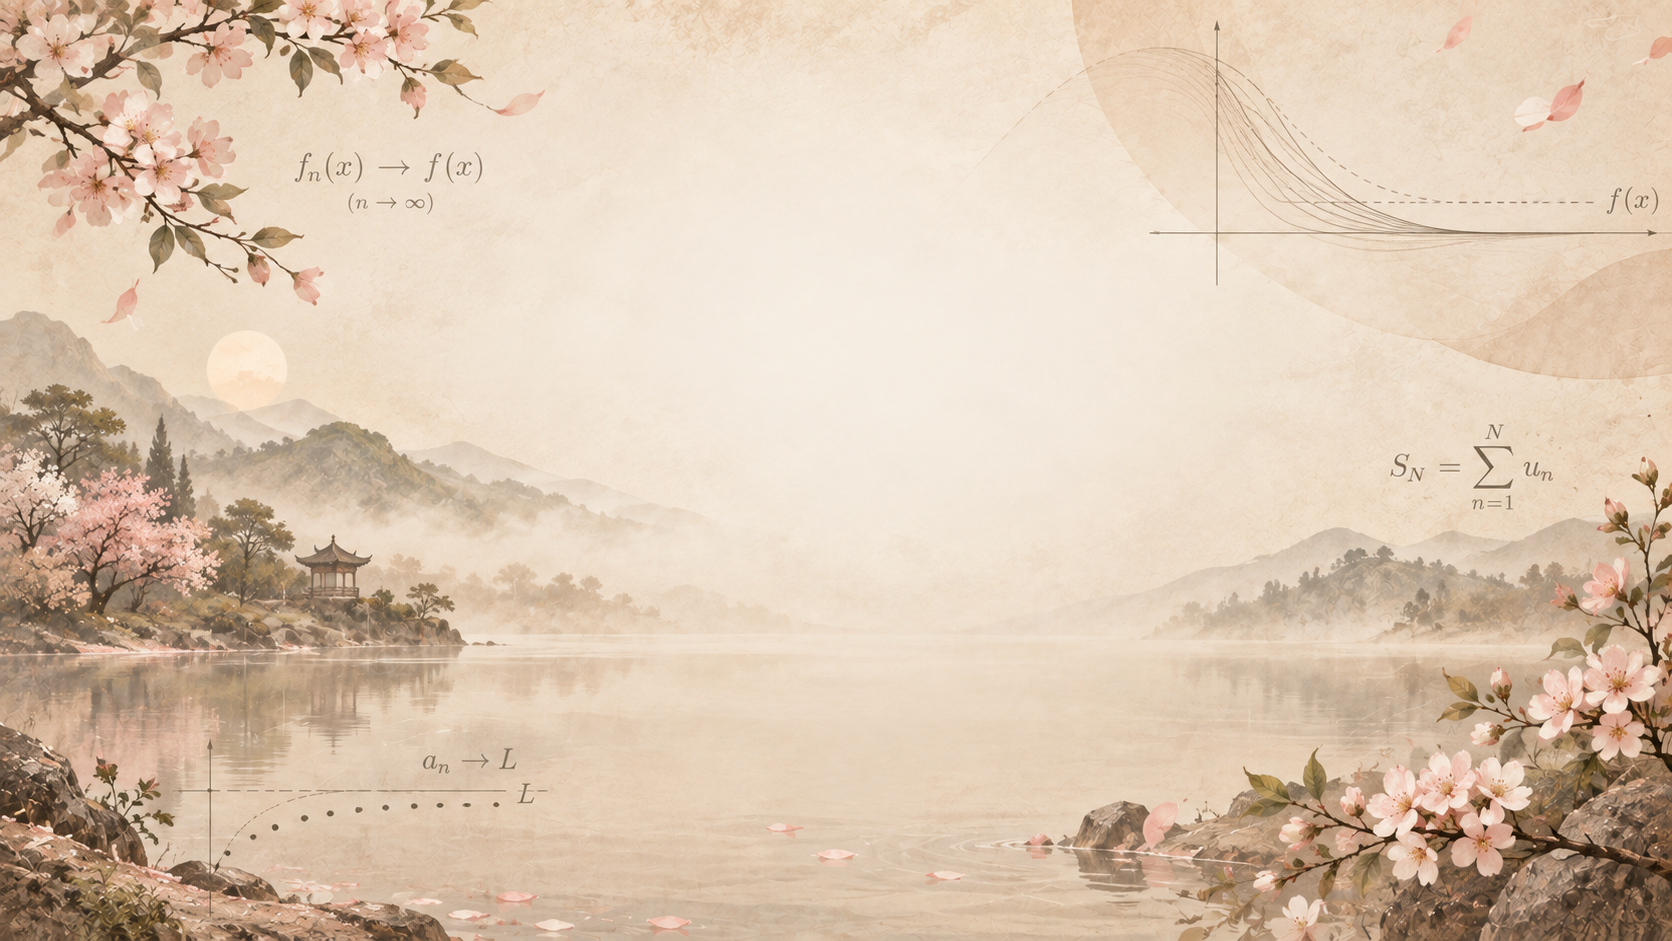
\includegraphics[width=\paperwidth,height=\paperheight,keepaspectratio=false]{chapter_07_bg_05.png}%
}
\section{Algebras of Functions}

% --- Build 1/2 ---
\begin{frame}{Definition 7.28: Algebra of Functions}
  \hl{\emph{Which properties of polynomials make the Weierstrass theorem possible?}}

  \vspace{0.4em}
  \begin{defblock}{Definition 7.28}
    A family $\mathscr{A}$ of complex functions defined on a set $E$ is an \alert{algebra} if,
    for all $f, g \in \mathscr{A}$ and all complex constants $c$,
    \[
      \text{(i)}\;\; f + g \in \mathscr{A}, \qquad
      \text{(ii)}\;\; fg \in \mathscr{A}, \qquad
      \text{(iii)}\;\; cf \in \mathscr{A},
    \]
    that is, $\mathscr{A}$ is closed under addition, multiplication, and scalar multiplication.
  \end{defblock}

  \note{
    We now isolate the relevant structure. Definition 7.28 says that a
    family of complex functions on a set capital "E", denoted by a script
    capital "A", is called an algebra if it is closed under three
    operations. Property 1: the sum of two members is a member. Property 2:
    the product of two members is a member. Property 3: a constant multiple
    of a member is a member. The products are taken pointwise. Notice what
    is not required: an algebra need not contain the constant functions, and
    the set capital "E" is completely arbitrary.
  }
\end{frame}

% --- Build 2/2 ---
\begin{frame}{Definition 7.28: Algebra of Functions}
  \hl{\emph{Which properties of polynomials make the Weierstrass theorem possible?}}

  \vspace{0.4em}
  \begin{defblock}{Definition 7.28}
    A family $\mathscr{A}$ of complex functions defined on a set $E$ is an \alert{algebra} if,
    for all $f, g \in \mathscr{A}$ and all complex constants $c$,
    \[
      \text{(i)}\;\; f + g \in \mathscr{A}, \qquad
      \text{(ii)}\;\; fg \in \mathscr{A}, \qquad
      \text{(iii)}\;\; cf \in \mathscr{A},
    \]
    that is, $\mathscr{A}$ is closed under addition, multiplication, and scalar multiplication.
  \end{defblock}
  \vspace{0.5em}
  \hl{\textbf{Real algebras:} real functions; (iii) is required only for real $c$.}

  \note{
    We will also work with algebras of real functions. In that case property
    3 is of course only required for real constants, since multiplying a
    real function by a complex number would take us out of the family.
    Stone's theorem will be proved first for real algebras. Next come two
    further notions from the same definition.
  }
\end{frame}

% --- Build 1/2 ---
\begin{frame}{Definition 7.28: Uniform Closure}
  \begin{defblock}{Definition 7.28 (continued)}
    $\mathscr{A}$ is \alert{uniformly closed} if $f \in \mathscr{A}$ whenever
    $f_n \in \mathscr{A}$ $(n = 1, 2, 3, \dots)$ and $f_n \to f$ uniformly on $E$.
  \end{defblock}

  \note{
    An algebra capital "A" is called uniformly closed if it contains all of
    its uniform limits. That is, whenever a sequence of members of capital
    "A" converges uniformly on capital "E" to some function "f", that limit
    "f" is again a member of capital "A". You cannot escape from a uniformly
    closed family by taking uniform limits.
  }
\end{frame}

% --- Build 2/2 ---
\begin{frame}{Definition 7.28: Uniform Closure}
  \begin{defblock}{Definition 7.28 (continued)}
    $\mathscr{A}$ is \alert{uniformly closed} if $f \in \mathscr{A}$ whenever
    $f_n \in \mathscr{A}$ $(n = 1, 2, 3, \dots)$ and $f_n \to f$ uniformly on $E$.

    \medskip
    The \alert{uniform closure} $\mathscr{B}$ of $\mathscr{A}$ is the set of all functions which are
    limits of uniformly convergent sequences of members of $\mathscr{A}$. (See Definition 7.14.)
  \end{defblock}
  \vspace{0.4em}
  \begin{center}
  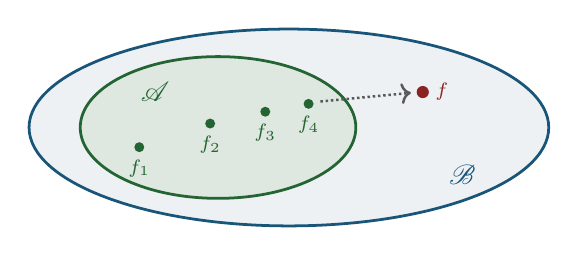
\begin{tikzpicture}[scale=1.0]
    \draw[defcolor, line width=1pt, fill=defcolor!8] (0,0) ellipse (3.3 and 1.25);
    \draw[proofcolor, line width=1pt, fill=proofcolor!15] (-0.9,0) ellipse (1.75 and 0.9);
    \node[defcolor] at (2.2,-0.6) {$\mathscr{B}$};
    \node[proofcolor] at (-1.7,0.45) {$\mathscr{A}$};
    \foreach \x/\y/\l in {-1.9/-0.25/1, -1.0/0.05/2, -0.3/0.2/3, 0.25/0.3/4}
      {\fill[proofcolor] (\x,\y) circle (1.8pt) node[below=1pt, font=\scriptsize] {$f_\l$};}
    \fill[thmcolor] (1.7,0.45) circle (2.2pt) node[right=1pt, font=\scriptsize] {$f$};
    \draw[->, gray!70!black, densely dotted, line width=0.9pt] (0.4,0.33) -- (1.55,0.44);
  \end{tikzpicture}
  \end{center}

  \note{
    If capital "A" is not uniformly closed, we can enlarge it. The uniform
    closure, denoted capital "B", consists of all functions that are uniform
    limits of sequences from capital "A". In the picture, the green region
    is capital "A" and the larger blue region is capital "B". The green dots
    form a sequence inside capital "A", and the dotted arrow shows it
    converging to the red point "f", which may lie outside capital "A" but
    belongs to capital "B". The reference to Definition 7.14 is a reminder
    that uniform convergence is convergence in the supremum metric, so for
    bounded functions the uniform closure is simply the closure in that
    metric space.
  }
\end{frame}

% --- Build 1/2 ---
\begin{frame}{Example: The Algebra of Polynomials}
  \begin{exblock}{Example}
    \begin{itemize}\setlength{\itemsep}{0.5em}
      \item The set of all polynomials is an \alert{algebra}.
    \end{itemize}
  \end{exblock}

  \note{
    The model example is the set of all polynomials. Sums, products, and
    constant multiples of polynomials are polynomials, so this set is an
    algebra. Restricted to an interval from "a" to "b", it is an algebra of
    continuous functions on that interval.
  }
\end{frame}

% --- Build 2/2 ---
\begin{frame}{Example: The Algebra of Polynomials}
  \begin{exblock}{Example}
    \begin{itemize}\setlength{\itemsep}{0.5em}
      \item The set of all polynomials is an \alert{algebra}.
      \item The Weierstrass theorem, restated:
        \[
          \text{uniform closure of the polynomials on } [a,b] \;=\; \mathscr{C}[a,b],
        \]
        the set of all continuous functions on $[a,b]$.
      \item The polynomials are \emph{not} uniformly closed: $|x|$ is a uniform limit of
        polynomials, but not a polynomial.
    \end{itemize}
  \end{exblock}

  \note{
    In this language, the Weierstrass theorem becomes a single equation. The
    uniform closure of the polynomials on the interval is the set of all
    continuous functions on the interval. One inclusion is Theorem 7.26. The
    other holds because a uniform limit of continuous functions is
    continuous, by Theorem 7.12. The last bullet notes that the polynomials
    themselves are not uniformly closed. By Corollary 7.27 the absolute
    value is a uniform limit of polynomials, yet it is not a polynomial.
    Next we prove that taking the uniform closure preserves the algebra
    structure.
  }
\end{frame}

% --- Build 1/3 ---
\begin{frame}{Theorem 7.29: The Closure of an Algebra}
  \small
  \begin{thmblock}{Theorem 7.29}
    Let $\mathscr{B}$ be the uniform closure of an algebra $\mathscr{A}$ of bounded functions.
    Then $\mathscr{B}$ is a uniformly closed algebra.
  \end{thmblock}

  \note{
    Theorem 7.29 says that the uniform closure of an algebra of bounded
    functions is again an algebra, and it is uniformly closed. So passing to
    the closure keeps the algebraic structure and adds closedness under
    uniform limits. Two things must be checked: that capital "B" is closed
    under the three algebraic operations, and that it is closed under
    uniform limits.
  }
\end{frame}

% --- Build 2/3 ---
\begin{frame}{Theorem 7.29: The Closure of an Algebra}
  \small
  \begin{thmblock}{Theorem 7.29}
    Let $\mathscr{B}$ be the uniform closure of an algebra $\mathscr{A}$ of bounded functions.
    Then $\mathscr{B}$ is a uniformly closed algebra.
  \end{thmblock}
  \vspace{0.1em}
  \begin{proofblock}{Proof: $\mathscr{B}$ is an algebra}
    Let $f, g \in \mathscr{B}$; choose $f_n, g_n \in \mathscr{A}$ with $f_n \to f$, $g_n \to g$ uniformly.
    By boundedness,
    \[
      f_n + g_n \to f + g, \qquad f_n g_n \to fg, \qquad c f_n \to cf
    \]
    uniformly, for any constant $c$. Hence $f + g$, $fg$, $cf \in \mathscr{B}$.\\[2pt]
    {\footnotesize (Product: $f_n g_n - fg = f_n (g_n - g) + g\,(f_n - f)$.)}
  \end{proofblock}

  \note{
    Take "f" and "g" in capital "B". By definition there are sequences in
    capital "A" converging to them uniformly. The sums, the products, and
    the constant multiples of these sequences lie in capital "A", because
    capital "A" is an algebra. They converge uniformly to the sum, the
    product, and the constant multiple of the limits. For sums and multiples
    this is immediate. For products we need boundedness. The identity in
    small print splits the error into two terms, each a bounded function
    times something uniformly small. So the three limits are in capital "B",
    and capital "B" is an algebra.
  }
\end{frame}

% --- Build 3/3 ---
\begin{frame}{Theorem 7.29: The Closure of an Algebra}
  \small
  \begin{thmblock}{Theorem 7.29}
    Let $\mathscr{B}$ be the uniform closure of an algebra $\mathscr{A}$ of bounded functions.
    Then $\mathscr{B}$ is a uniformly closed algebra.
  \end{thmblock}
  \vspace{0.1em}
  \begin{proofblock}{Proof: $\mathscr{B}$ is an algebra}
    Let $f, g \in \mathscr{B}$; choose $f_n, g_n \in \mathscr{A}$ with $f_n \to f$, $g_n \to g$ uniformly.
    By boundedness,
    \[
      f_n + g_n \to f + g, \qquad f_n g_n \to fg, \qquad c f_n \to cf
    \]
    uniformly, for any constant $c$. Hence $f + g$, $fg$, $cf \in \mathscr{B}$.\\[2pt]
    {\footnotesize (Product: $f_n g_n - fg = f_n (g_n - g) + g\,(f_n - f)$.)}
  \end{proofblock}

  \vspace{0.1em}
  \begin{proofblock}{Proof: $\mathscr{B}$ is uniformly closed}
    By Theorem 2.27, the closure of a set is closed. \hfill $\blacksquare$
  \end{proofblock}

  \note{
    For the second part, recall Theorem 2.27 from Chapter 2: in any metric
    space, the closure of a set is a closed set. Here the metric space is
    the space of bounded functions on capital "E" with the supremum metric,
    and capital "B" is the closure of capital "A" in it. So capital "B" is
    closed, which means precisely that it is uniformly closed. A uniform
    limit of uniform limits is still a uniform limit. That completes the
    proof. Being an algebra is not enough for approximation, so next we add
    two conditions.
  }
\end{frame}
}

{
\usebackgroundtemplate{%
  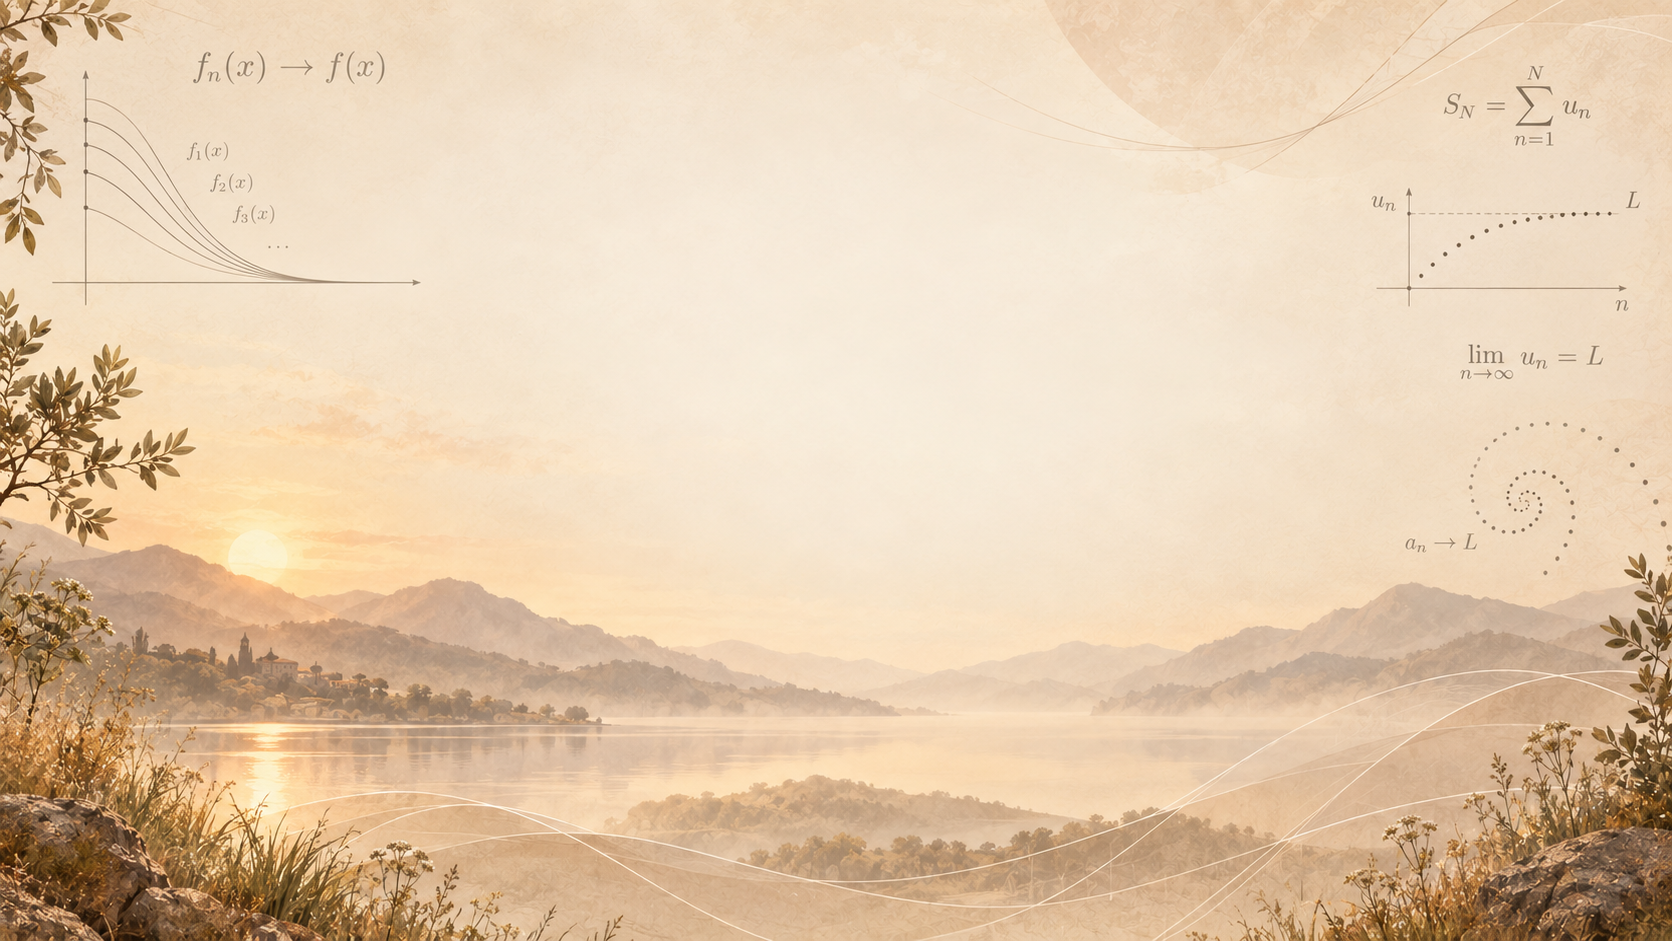
\includegraphics[width=\paperwidth,height=\paperheight,keepaspectratio=false]{chapter_07_bg_06.png}%
}
\section{Separating Points}

% --- Build 1/2 ---
\begin{frame}{Definition 7.30: Separating Points}
  \begin{defblock}{Definition 7.30}
    Let $\mathscr{A}$ be a family of functions on a set $E$.

    \medskip
    $\mathscr{A}$ \alert{separates points} on $E$ if to every pair of distinct points
    $x_1, x_2 \in E$ there corresponds a function $f \in \mathscr{A}$ such that
    $f(x_1) \ne f(x_2)$.
  \end{defblock}

  \note{
    Definition 7.30 introduces two properties of a family of functions. The
    first: capital "A" separates points on capital "E" if, for any two
    distinct points "x" sub 1 and "x" sub 2, some function in the family
    takes different values at them. In other words, the family as a whole
    can tell any two points apart. The function is allowed to depend on the
    pair of points.
  }
\end{frame}

% --- Build 2/2 ---
\begin{frame}{Definition 7.30: Separating Points}
  \begin{defblock}{Definition 7.30}
    Let $\mathscr{A}$ be a family of functions on a set $E$.

    \medskip
    $\mathscr{A}$ \alert{separates points} on $E$ if to every pair of distinct points
    $x_1, x_2 \in E$ there corresponds a function $f \in \mathscr{A}$ such that
    $f(x_1) \ne f(x_2)$.

    \medskip
    $\mathscr{A}$ \alert{vanishes at no point of $E$} if to each $x \in E$ there
    corresponds a function $g \in \mathscr{A}$ such that $g(x) \ne 0$.
  \end{defblock}
  \vspace{0.6em}
  \begin{hlbox}
  The functions $f$ and $g$ may depend on the points --- no single function has to do everything.
  \end{hlbox}

  \note{
    The second: capital "A" vanishes at no point of capital "E" if, for each
    point "x", some function "g" in the family is nonzero at "x". So there
    is no point at which every member of the family is zero. Again, the
    function may depend on the point. No single member has to be nonzero
    everywhere. Let's look at examples.
  }
\end{frame}

% --- Build 1/2 ---
\begin{frame}{Examples: All Polynomials vs.\ Even Polynomials}
  \begin{columns}[T]
    \begin{column}{0.48\textwidth}
      \begin{exblock}{All polynomials on $R^1$}
        \begin{itemize}
          \item \textbf{Separate points:} $f(x) = x$ works for every pair.
          \item \textbf{Vanish at no point:} $g(x) = 1$ works for every point.
        \end{itemize}
      \end{exblock}
    \end{column}
    \begin{column}{0.48\textwidth}

    \end{column}
  \end{columns}

  \note{
    The algebra of all polynomials in one variable clearly has both
    properties on the real line. To separate two distinct points, use the
    polynomial "f" of "x" equals "x". It takes different values at different
    points. And the constant polynomial 1 is nonzero at every point, so the
    algebra vanishes nowhere. Here a single function happens to do the job
    in each case.
  }
\end{frame}

% --- Build 2/2 ---
\begin{frame}{Examples: All Polynomials vs.\ Even Polynomials}
  \begin{columns}[T]
    \begin{column}{0.48\textwidth}
      \begin{exblock}{All polynomials on $R^1$}
        \begin{itemize}
          \item \textbf{Separate points:} $f(x) = x$ works for every pair.
          \item \textbf{Vanish at no point:} $g(x) = 1$ works for every point.
        \end{itemize}
      \end{exblock}
    \end{column}
    \begin{column}{0.48\textwidth}
      \begin{exblock}{Even polynomials on $[-1,1]$}
        $f(-x) = f(x)$ for every even $f$\\
        $\Longrightarrow$ they do \alert{not} separate $x$ and $-x$.

        \centering
        \smallskip
  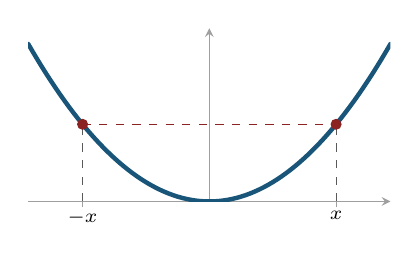
\begin{tikzpicture}
    \begin{axis}[swaxis, width=4.6cm, height=2.2cm, xmin=-1, xmax=1, ymin=0, ymax=1.1,
        axis y line=middle, xtick={-0.7,0.7}, xticklabels={$-x$,$x$}, ytick=\empty, samples=81]
      \addplot[defcolor, curveln, domain=-1:1] {x^2};
      \draw[thmcolor, dashed] (axis cs:-0.7,0.49) -- (axis cs:0.7,0.49);
      \draw[gray!70!black, dashed] (axis cs:-0.7,0) -- (axis cs:-0.7,0.49);
      \draw[gray!70!black, dashed] (axis cs:0.7,0) -- (axis cs:0.7,0.49);
      \fill[thmcolor] (axis cs:-0.7,0.49) circle (2pt);
      \fill[thmcolor] (axis cs:0.7,0.49) circle (2pt);
    \end{axis}
  \end{tikzpicture}
      \end{exblock}
    \end{column}
  \end{columns}

  \note{
    For contrast, consider the even polynomials, those containing only even
    powers of "x", on the interval from minus 1 to 1. They form an algebra.
    But every even function takes the same value at "x" and at minus "x".
    The picture shows the blue graph of "x" squared, with two red dots at
    the same height above minus "x" and above "x", joined by a dashed line.
    No member of this algebra can tell these two points apart, so it does
    not separate points. Why should we care about these properties?
  }
\end{frame}

% --- Build 1/2 ---
\begin{frame}{Why These Two Conditions?}
  \begin{remblock}{If $\mathscr{A}$ fails to separate $x_1 \ne x_2$}
    Every $f \in \mathscr{A}$ has $f(x_1) = f(x_2)$ --- and so does every uniform limit.\\
    A continuous function with different values at $x_1$, $x_2$ cannot be approximated.
  \end{remblock}

  \note{
    These conditions are not arbitrary. They are necessary for any
    approximation theorem. Suppose capital "A" fails to separate two points.
    Then every member takes equal values at those two points. That equality
    survives uniform limits, even pointwise limits. So every function in the
    uniform closure also takes equal values there. A continuous function
    with different values at the two points can never be reached. For
    instance, even polynomials can only approximate even functions.
  }
\end{frame}

% --- Build 2/2 ---
\begin{frame}{Why These Two Conditions?}
  \begin{remblock}{If $\mathscr{A}$ fails to separate $x_1 \ne x_2$}
    Every $f \in \mathscr{A}$ has $f(x_1) = f(x_2)$ --- and so does every uniform limit.\\
    A continuous function with different values at $x_1$, $x_2$ cannot be approximated.
  \end{remblock}

  \vspace{0.5em}
  \begin{remblock}{If every $f \in \mathscr{A}$ vanishes at some $x_0$}
    Every uniform limit vanishes at $x_0$.\\
    The constant function $1$ cannot be approximated.
  \end{remblock}

  \vspace{0.7em}
  \begin{hlbox}
  Both conditions are \alert{necessary}. Stone's theorem: on compact sets, they are also \alert{sufficient}.
  \end{hlbox}

  \note{
    Similarly, suppose every member of capital "A" vanishes at some point
    "x" sub 0. Then every uniform limit vanishes there too, and the constant
    function 1 cannot be approximated. So both conditions are necessary if
    we hope to approximate all continuous functions. The beautiful content
    of Stone's theorem is the converse: for an algebra of real continuous
    functions on a compact set, these two obvious necessary conditions are
    already sufficient. The bridge is the next theorem.
  }
\end{frame}

% --- Build 1/2 ---
\begin{frame}{Theorem 7.31: Two-Point Interpolation}
  \begin{thmblock}{Theorem 7.31}
    Suppose $\mathscr{A}$ is an algebra of functions on a set $E$, $\mathscr{A}$ separates points
    on $E$, and $\mathscr{A}$ vanishes at no point of $E$. Suppose $x_1$, $x_2$ are distinct
    points of $E$, and $c_1$, $c_2$ are constants (real if $\mathscr{A}$ is a real algebra).
    Then $\mathscr{A}$ contains a function $f$ such that
    \[
      f(x_1) = c_1, \qquad f(x_2) = c_2 .
    \]
  \end{thmblock}

  \note{
    Theorem 7.31 shows what the two conditions buy us when combined with the
    algebra structure. Let capital "A" be an algebra that separates points
    and vanishes at no point of capital "E". Pick two distinct points, "x"
    sub 1 and "x" sub 2, and any two target values, "c" sub 1 and "c" sub 2.
    Then some function in capital "A" takes exactly the value "c" sub 1 at
    the first point and "c" sub 2 at the second.
  }
\end{frame}

% --- Build 2/2 ---
\begin{frame}{Theorem 7.31: Two-Point Interpolation}
  \begin{thmblock}{Theorem 7.31}
    Suppose $\mathscr{A}$ is an algebra of functions on a set $E$, $\mathscr{A}$ separates points
    on $E$, and $\mathscr{A}$ vanishes at no point of $E$. Suppose $x_1$, $x_2$ are distinct
    points of $E$, and $c_1$, $c_2$ are constants (real if $\mathscr{A}$ is a real algebra).
    Then $\mathscr{A}$ contains a function $f$ such that
    \[
      f(x_1) = c_1, \qquad f(x_2) = c_2 .
    \]
  \end{thmblock}
  \begin{center}
  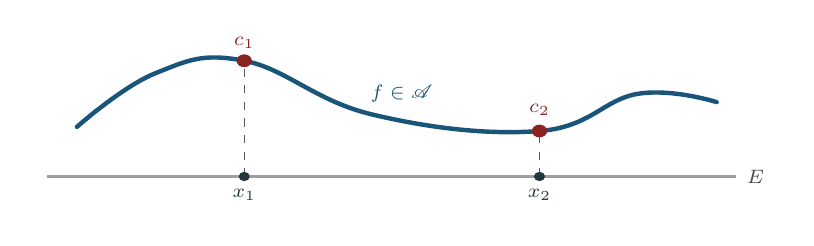
\begin{tikzpicture}[xscale=1.25, yscale=1.05]
    \fill[white, opacity=0.6] (-0.2,-0.5) rectangle (7.5,1.8);
    \draw[gray!75, line width=0.9pt] (0,0) -- (7,0) node[right, font=\scriptsize, text=gray!60!black] {$E$};
    \draw[defcolor, curveln] plot[smooth, tension=0.7] coordinates {(0.3,0.6) (1.1,1.25) (2,1.4) (3.3,0.75) (5,0.55) (6,1.0) (6.8,0.9)};
    \draw[gray!70!black, dashed] (2,0) -- (2,1.4);
    \draw[gray!70!black, dashed] (5,0) -- (5,0.55);
    \fill[thmcolor] (2,1.4) circle (2.2pt) node[above=1pt, font=\scriptsize] {$c_1$};
    \fill[thmcolor] (5,0.55) circle (2.2pt) node[above=2pt, font=\scriptsize] {$c_2$};
    \fill[mDarkTeal] (2,0) circle (1.6pt) node[below=1pt, font=\scriptsize] {$x_1$};
    \fill[mDarkTeal] (5,0) circle (1.6pt) node[below=1pt, font=\scriptsize] {$x_2$};
    \node[defcolor, font=\scriptsize] at (3.6,1.0) {$f \in \mathscr{A}$};
  \end{tikzpicture}
  \end{center}

  \note{
    The picture illustrates this. The horizontal line stands for the set
    capital "E", the red dots are the prescribed values above the two
    points, and the blue curve is a member of the algebra passing through
    both. So the algebra can interpolate any values at any two points. We
    have no control elsewhere, but two points will be enough. Let's prove
    it.
  }
\end{frame}

% --- Build 1/3 ---
\begin{frame}{Proof of Theorem 7.31}
  \begin{proofblock}{Proof}
    The assumptions show that $\mathscr{A}$ contains functions $g$, $h$, $k$ such that
    \[
      g(x_1) \ne g(x_2), \qquad h(x_1) \ne 0, \qquad k(x_2) \ne 0 .
    \]
  \end{proofblock}

  \note{
    The hypotheses hand us three functions in the algebra. Since capital "A"
    separates points, there is a function "g" with different values at "x"
    sub 1 and "x" sub 2. Since capital "A" vanishes at no point, there is a
    function "h" that is nonzero at "x" sub 1, and a function "k" that is
    nonzero at "x" sub 2. We now combine them.
  }
\end{frame}

% --- Build 2/3 ---
\begin{frame}{Proof of Theorem 7.31}
  \begin{proofblock}{Proof}
    The assumptions show that $\mathscr{A}$ contains functions $g$, $h$, $k$ such that
    \[
      g(x_1) \ne g(x_2), \qquad h(x_1) \ne 0, \qquad k(x_2) \ne 0 .
    \]
    Put
    \[
      u = gk - g(x_1)\,k, \qquad v = gh - g(x_2)\,h .
    \]
    Then $u, v \in \mathscr{A}$, \; $u(x_1) = v(x_2) = 0$, \; $u(x_2) \ne 0$, \; $v(x_1) \ne 0$.
  \end{proofblock}

  \note{
    Define "u" and "v" as on the slide. Each is a product of two members
    minus a constant multiple of a member, so both belong to capital "A".
    Note that we never use constant functions. We can factor "u" as "k"
    times the difference "g" minus "g" of "x" sub 1. At "x" sub 1 the second
    factor vanishes, so "u" is zero there. At "x" sub 2 both factors are
    nonzero, so "u" is nonzero. Symmetrically, "v" vanishes at "x" sub 2 and
    is nonzero at "x" sub 1.
  }
\end{frame}

% --- Build 3/3 ---
\begin{frame}{Proof of Theorem 7.31}
  \begin{proofblock}{Proof}
    The assumptions show that $\mathscr{A}$ contains functions $g$, $h$, $k$ such that
    \[
      g(x_1) \ne g(x_2), \qquad h(x_1) \ne 0, \qquad k(x_2) \ne 0 .
    \]
    Put
    \[
      u = gk - g(x_1)\,k, \qquad v = gh - g(x_2)\,h .
    \]
    Then $u, v \in \mathscr{A}$, \; $u(x_1) = v(x_2) = 0$, \; $u(x_2) \ne 0$, \; $v(x_1) \ne 0$.
    Therefore
    \[
      f = \frac{c_1\,v}{v(x_1)} + \frac{c_2\,u}{u(x_2)}
    \]
    has the desired properties. \hfill $\blacksquare$
  \end{proofblock}
  \vspace{0.1em}
  \begin{hlbox}
  \small \textbf{Idea:} $u$ and $v$ act as switches --- $v$ is ``on'' at $x_1$ and ``off'' at $x_2$; $u$ the reverse.
  \end{hlbox}

  \note{
    Finally, define "f" as the combination on the slide. It is a sum of
    constant multiples of "v" and "u", so it lies in capital "A". At "x" sub
    1 the function "u" vanishes and the first term gives exactly "c" sub 1.
    At "x" sub 2 the function "v" vanishes and the second term gives "c" sub
    2. The idea is that "u" and "v" act as switches. One is on at the first
    point and off at the second, and the other does the reverse. This is the
    same idea as Lagrange interpolation. We now have everything needed for
    Stone's theorem.
  }
\end{frame}
}

{
\usebackgroundtemplate{%
  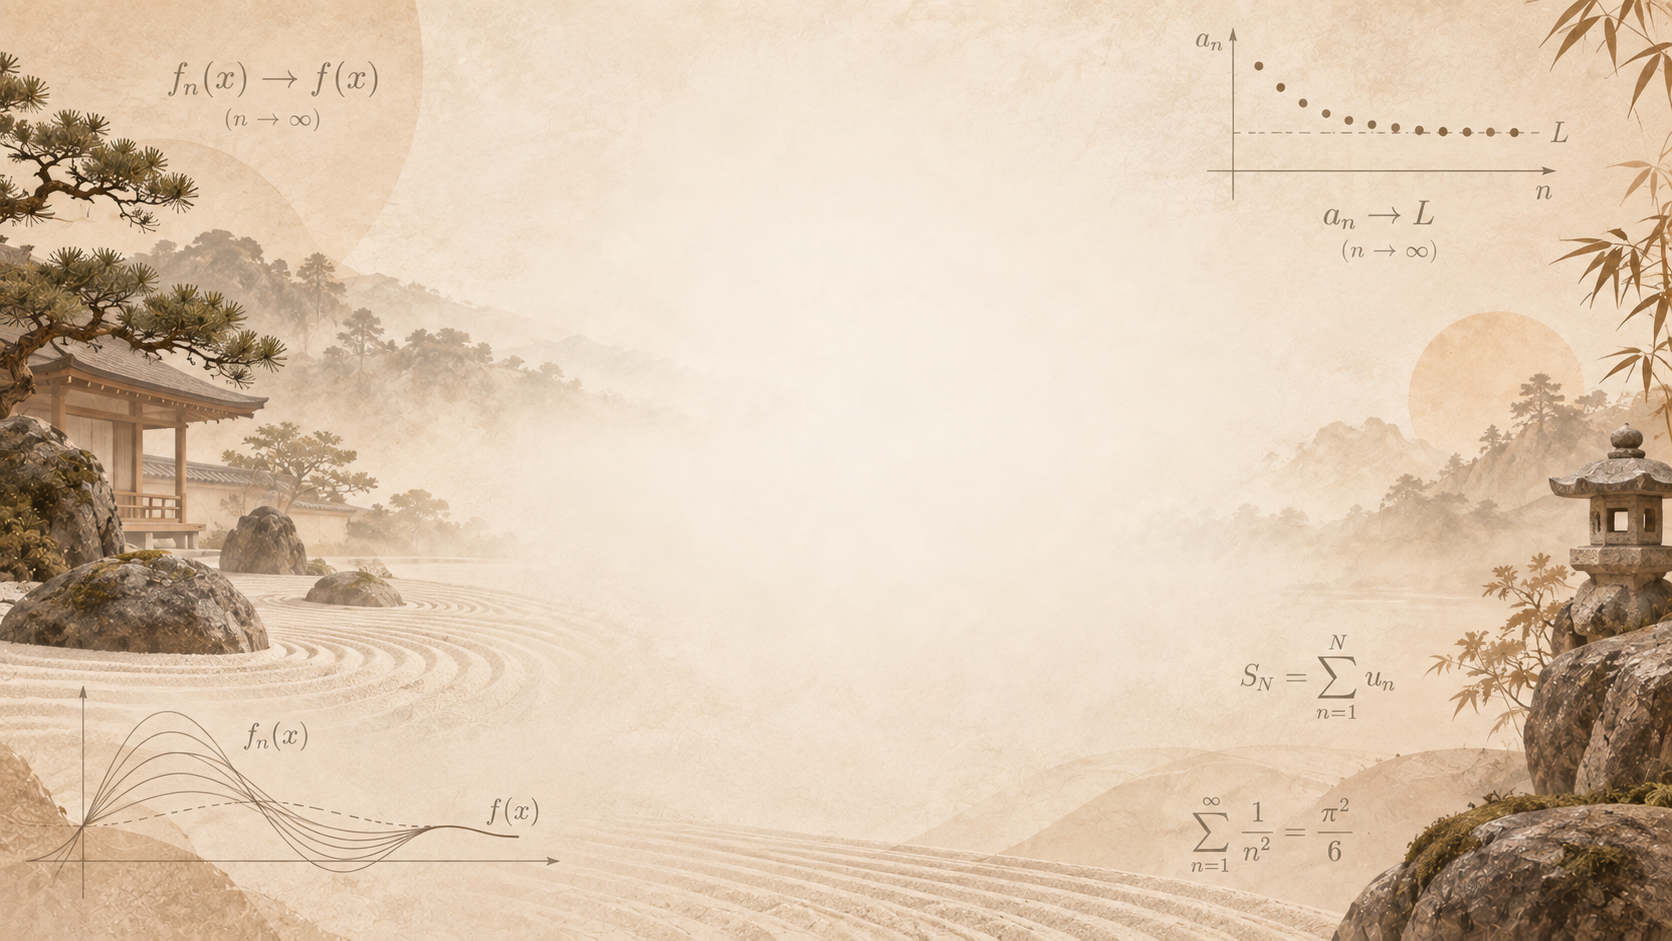
\includegraphics[width=\paperwidth,height=\paperheight,keepaspectratio=false]{chapter_07_bg_07.png}%
}
\section{Stone's Theorem}

% --- Build 1/2 ---
\begin{frame}{Theorem 7.32: The Stone--Weierstrass Theorem}
  \begin{thmblock}{Theorem 7.32}
    Let $\mathscr{A}$ be an algebra of real continuous functions on a compact set $K$.
    If $\mathscr{A}$ separates points on $K$ and if $\mathscr{A}$ vanishes at no point of $K$,
    then the uniform closure $\mathscr{B}$ of $\mathscr{A}$ consists of \alert{all} real
    continuous functions on $K$.
  \end{thmblock}

  \note{
    Here is Stone's generalization of the Weierstrass theorem. Let capital
    "A" be an algebra of real continuous functions on a compact set capital
    "K". Assume it separates points and vanishes at no point of capital "K".
    Then its uniform closure, capital "B", is the set of all real continuous
    functions on capital "K". In other words, every real continuous function
    on capital "K" can be approximated uniformly, as closely as we like, by
    members of capital "A". Notice how little is assumed about capital "K".
    It is any compact metric space, not just an interval.
  }
\end{frame}

% --- Build 2/2 ---
\begin{frame}{Theorem 7.32: The Stone--Weierstrass Theorem}
  \begin{thmblock}{Theorem 7.32}
    Let $\mathscr{A}$ be an algebra of real continuous functions on a compact set $K$.
    If $\mathscr{A}$ separates points on $K$ and if $\mathscr{A}$ vanishes at no point of $K$,
    then the uniform closure $\mathscr{B}$ of $\mathscr{A}$ consists of \alert{all} real
    continuous functions on $K$.
  \end{thmblock}
  \vspace{0.6em}
  \begin{exblock}{Special cases}
    \begin{itemize}
      \item $K = [a,b]$, $\mathscr{A}$ = real polynomials: the Weierstrass theorem.
      \item $K \subset R^k$ compact, $\mathscr{A}$ = real polynomials in $k$ variables.
    \end{itemize}
  \end{exblock}

  \note{
    Two special cases show the scope. If capital "K" is a closed interval
    and capital "A" is the algebra of real polynomials, we recover the real
    case of the Weierstrass theorem, since we checked that polynomials
    separate points and vanish nowhere. If capital "K" is a compact subset
    of Euclidean space of dimension "k", the polynomials in "k" variables
    form an algebra with both properties, since the coordinate functions
    separate points. So continuous functions of several variables are
    uniform limits of polynomials on compact sets. Our kernel proof would
    not give this directly. Let's look at the strategy.
  }
\end{frame}

% --- Build 1/4 ---
\begin{frame}{Proof Strategy: Theorem 7.32}
  \begin{hlbox}
  \textbf{Goal:} every real continuous $f$ on $K$ lies in $\mathscr{B}$
  {\small (a uniformly closed algebra, by Theorem 7.29).}

  \vspace{0.8em}
  \textbf{Step 1.}\;\; $f \in \mathscr{B} \;\Longrightarrow\; |f| \in \mathscr{B}$
  \hfill {\small (Corollary 7.27)}\par\vspace{0.7em}
  \end{hlbox}

  \note{
    Rudin divides the proof into four steps. Throughout, we work in the
    closure capital "B", which by Theorem 7.29 is a uniformly closed
    algebra. Continuous functions on a compact set are bounded, so that
    theorem applies. Step 1 shows that capital "B" is closed under taking
    absolute values. This is where the Weierstrass theorem enters, through
    Corollary 7.27.
  }
\end{frame}

% --- Build 2/4 ---
\begin{frame}{Proof Strategy: Theorem 7.32}
  \begin{hlbox}
  \textbf{Goal:} every real continuous $f$ on $K$ lies in $\mathscr{B}$
  {\small (a uniformly closed algebra, by Theorem 7.29).}

  \vspace{0.8em}
  \textbf{Step 1.}\;\; $f \in \mathscr{B} \;\Longrightarrow\; |f| \in \mathscr{B}$
  \hfill {\small (Corollary 7.27)}\par\vspace{0.7em}
  \textbf{Step 2.}\;\; $f, g \in \mathscr{B} \;\Longrightarrow\; \max(f,g),\ \min(f,g) \in \mathscr{B}$
  \hfill {\small (Step 1)}\par\vspace{0.7em}
  \end{hlbox}

  \note{
    Step 2 upgrades this: capital "B" is closed under taking the pointwise
    maximum and the pointwise minimum of two functions, and hence of
    finitely many. These are lattice operations. They are not algebraic
    operations, but they can be expressed through the absolute value. They
    let us glue functions together.
  }
\end{frame}

% --- Build 3/4 ---
\begin{frame}{Proof Strategy: Theorem 7.32}
  \begin{hlbox}
  \textbf{Goal:} every real continuous $f$ on $K$ lies in $\mathscr{B}$
  {\small (a uniformly closed algebra, by Theorem 7.29).}

  \vspace{0.8em}
  \textbf{Step 1.}\;\; $f \in \mathscr{B} \;\Longrightarrow\; |f| \in \mathscr{B}$
  \hfill {\small (Corollary 7.27)}\par\vspace{0.7em}
  \textbf{Step 2.}\;\; $f, g \in \mathscr{B} \;\Longrightarrow\; \max(f,g),\ \min(f,g) \in \mathscr{B}$
  \hfill {\small (Step 1)}\par\vspace{0.7em}
  \textbf{Step 3.}\;\; $g_x \in \mathscr{B}$ with $g_x(x) = f(x)$, \;$g_x > f - \varepsilon$ on $K$
  \hfill {\small (7.31, compactness)}\par\vspace{0.7em}
  \end{hlbox}

  \note{
    Step 3 is a one sided approximation. Fix a continuous target "f", a
    point "x", and epsilon. We construct a function "g" sub "x" in capital
    "B" that agrees with "f" at the point "x" and stays above "f" minus
    epsilon everywhere on capital "K". The tools are two point
    interpolation, a maximum, and compactness.
  }
\end{frame}

% --- Build 4/4 ---
\begin{frame}{Proof Strategy: Theorem 7.32}
  \begin{hlbox}
  \textbf{Goal:} every real continuous $f$ on $K$ lies in $\mathscr{B}$
  {\small (a uniformly closed algebra, by Theorem 7.29).}

  \vspace{0.8em}
  \textbf{Step 1.}\;\; $f \in \mathscr{B} \;\Longrightarrow\; |f| \in \mathscr{B}$
  \hfill {\small (Corollary 7.27)}\par\vspace{0.7em}
  \textbf{Step 2.}\;\; $f, g \in \mathscr{B} \;\Longrightarrow\; \max(f,g),\ \min(f,g) \in \mathscr{B}$
  \hfill {\small (Step 1)}\par\vspace{0.7em}
  \textbf{Step 3.}\;\; $g_x \in \mathscr{B}$ with $g_x(x) = f(x)$, \;$g_x > f - \varepsilon$ on $K$
  \hfill {\small (7.31, compactness)}\par\vspace{0.7em}
  \textbf{Step 4.}\;\; Some $h \in \mathscr{B}$ has $|h - f| < \varepsilon$ on $K$
  \hfill {\small (compactness again)}
  \end{hlbox}

  \note{
    Step 4 takes care of the other side. Using a minimum of finitely many of
    the functions from Step 3, and compactness a second time, we get a
    function "h" in capital "B" within epsilon of "f" everywhere. Since
    capital "B" is uniformly closed, "f" itself belongs to capital "B".
    Let's go through the steps.
  }
\end{frame}

% --- Build 1/3 ---
\begin{frame}{Proof of Theorem 7.32 --- Step 1}
  \small
  \begin{proofblock}{Step 1: If $f \in \mathscr{B}$, then $|f| \in \mathscr{B}$}
    Let \quad $a = \sup |f(x)| \quad (x \in K)$ \hfill (52)\\[2pt]
    and let $\varepsilon > 0$ be given. By Corollary 7.27 there exist real numbers
    $c_1, \dots, c_n$ such that
    \[
      \Bigl| \sum_{i=1}^{n} c_i\,y^i - |y| \Bigr| < \varepsilon \qquad (-a \le y \le a). \tag{53}
    \]
  \end{proofblock}

  \note{
    Step 1. Let "f" be in capital "B", and let "a" be the supremum of its
    absolute value on capital "K", which is equation 52. So all values of
    "f" lie in the interval from minus "a" to "a". Given epsilon, Corollary
    7.27 provides a polynomial in a variable "y" that is within epsilon of
    the absolute value of "y" on that whole interval. This is equation 53.
    Notice that the sum starts with the first power of "y". There is no
    constant term, because the polynomial vanishes at zero.
  }
\end{frame}

% --- Build 2/3 ---
\begin{frame}{Proof of Theorem 7.32 --- Step 1}
  \small
  \begin{proofblock}{Step 1: If $f \in \mathscr{B}$, then $|f| \in \mathscr{B}$}
    Let \quad $a = \sup |f(x)| \quad (x \in K)$ \hfill (52)\\[2pt]
    and let $\varepsilon > 0$ be given. By Corollary 7.27 there exist real numbers
    $c_1, \dots, c_n$ such that
    \[
      \Bigl| \sum_{i=1}^{n} c_i\,y^i - |y| \Bigr| < \varepsilon \qquad (-a \le y \le a). \tag{53}
    \]

    Since $\mathscr{B}$ is an algebra, the function $\;g = \sum_{i=1}^{n} c_i\,f^i\;$ is a member of $\mathscr{B}$.
  \end{proofblock}

  \note{
    Now substitute "f" for "y". The function "g" is a linear combination of
    powers of "f". Since capital "B" is an algebra, products of "f" with
    itself are in capital "B", and so is any linear combination of them.
    Here we see why the missing constant term matters. A nonzero constant
    function might not belong to capital "B", but positive powers of "f"
    certainly do.
  }
\end{frame}

% --- Build 3/3 ---
\begin{frame}{Proof of Theorem 7.32 --- Step 1}
  \small
  \begin{proofblock}{Step 1: If $f \in \mathscr{B}$, then $|f| \in \mathscr{B}$}
    Let \quad $a = \sup |f(x)| \quad (x \in K)$ \hfill (52)\\[2pt]
    and let $\varepsilon > 0$ be given. By Corollary 7.27 there exist real numbers
    $c_1, \dots, c_n$ such that
    \[
      \Bigl| \sum_{i=1}^{n} c_i\,y^i - |y| \Bigr| < \varepsilon \qquad (-a \le y \le a). \tag{53}
    \]

    Since $\mathscr{B}$ is an algebra, the function $\;g = \sum_{i=1}^{n} c_i\,f^i\;$ is a member of $\mathscr{B}$.

    By (52) and (53), we have
    \[
      \bigl| g(x) - |f(x)| \bigr| < \varepsilon \qquad (x \in K).
    \]
    Since $\mathscr{B}$ is uniformly closed, this shows that $|f| \in \mathscr{B}$.
  \end{proofblock}

  \note{
    For each "x" in capital "K", the number "f" of "x" lies between minus
    "a" and "a", by equation 52. So we may put "y" equal to "f" of "x" in
    equation 53. The result is that "g" is within epsilon of the absolute
    value of "f" at every point of capital "K". Since epsilon was arbitrary,
    the absolute value of "f" is a uniform limit of members of capital "B".
    And capital "B" is uniformly closed, so it contains the absolute value
    of "f". That completes Step 1.
  }
\end{frame}

% --- Build 1/3 ---
\begin{frame}{Proof of Theorem 7.32 --- Step 2}
  \begin{columns}[T]
    \begin{column}{0.6\textwidth}
      \small
      \begin{proofblock}{Step 2}
        \raggedright
        If $f, g \in \mathscr{B}$, then $\max(f,g) \in \mathscr{B}$ and $\min(f,g) \in \mathscr{B}$.

        \smallskip
        Here $\max(f,g)$ is the function $h$ with
        \[
          h(x) = \begin{cases} f(x) & \text{if } f(x) \ge g(x), \\ g(x) & \text{if } f(x) < g(x), \end{cases}
        \]
        and $\min(f,g)$ is defined likewise.
      \end{proofblock}
    \end{column}
    \begin{column}{0.38\textwidth}
      \centering
  \vspace{0.8em}
  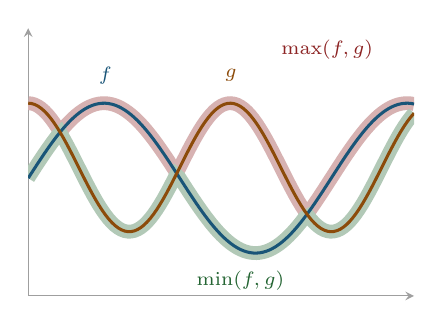
\begin{tikzpicture}
    \begin{axis}[swaxis, width=4.9cm, height=3.4cm, xmin=0, xmax=4, ymin=0, ymax=1.25,
        xtick=\empty, ytick=\empty, samples=121, domain=0:4]
      \addplot[thmcolor!35, line width=5pt] {max(0.55+0.35*sin(deg(2*x)), 0.6+0.3*cos(deg(3*x)))};
      \addplot[proofcolor!35, line width=5pt] {min(0.55+0.35*sin(deg(2*x)), 0.6+0.3*cos(deg(3*x)))};
      \addplot[defcolor, line width=1.1pt] {0.55+0.35*sin(deg(2*x))};
      \addplot[excolor, line width=1.1pt] {0.6+0.3*cos(deg(3*x))};
      \node[defcolor, font=\scriptsize] at (axis cs:0.8,1.03) {$f$};
      \node[excolor, font=\scriptsize] at (axis cs:2.1,1.03) {$g$};
      \node[thmcolor, font=\scriptsize] at (axis cs:3.1,1.15) {$\max(f,g)$};
      \node[proofcolor, font=\scriptsize] at (axis cs:2.2,0.07) {$\min(f,g)$};
    \end{axis}
  \end{tikzpicture}
    \end{column}
  \end{columns}

  \note{
    Step 2 concerns maximum and minimum. The maximum of "f" and "g" is the
    function "h" whose value at each point is the larger of the two values,
    and the minimum is defined likewise with the smaller value. In the
    picture, "f" is the thin blue curve and "g" is the thin amber curve. The
    wide red band follows whichever curve is on top, so it traces the
    maximum. The wide green band follows the lower one, so it traces the
    minimum. The claim is that if "f" and "g" are in capital "B", so are
    these two functions.
  }
\end{frame}

% --- Build 2/3 ---
\begin{frame}{Proof of Theorem 7.32 --- Step 2}
  \begin{columns}[T]
    \begin{column}{0.6\textwidth}
      \small
      \begin{proofblock}{Step 2}
        \raggedright
        If $f, g \in \mathscr{B}$, then $\max(f,g) \in \mathscr{B}$ and $\min(f,g) \in \mathscr{B}$.

        \smallskip
        Here $\max(f,g)$ is the function $h$ with
        \[
          h(x) = \begin{cases} f(x) & \text{if } f(x) \ge g(x), \\ g(x) & \text{if } f(x) < g(x), \end{cases}
        \]
        and $\min(f,g)$ is defined likewise.

        \smallskip
        \textbf{Proof.} Step 1 and the identities
        \[
          \max(f,g) = \tfrac{f+g}{2} + \tfrac{|f-g|}{2}, \quad
          \min(f,g) = \tfrac{f+g}{2} - \tfrac{|f-g|}{2}.
        \]
      \end{proofblock}
    \end{column}
    \begin{column}{0.38\textwidth}
      \centering
  \vspace{0.8em}
  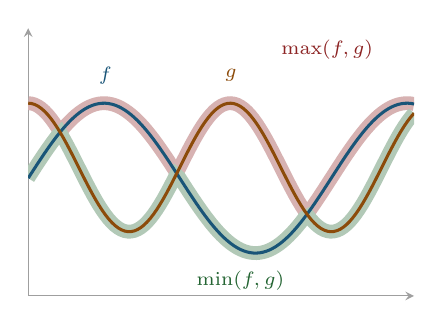
\begin{tikzpicture}
    \begin{axis}[swaxis, width=4.9cm, height=3.4cm, xmin=0, xmax=4, ymin=0, ymax=1.25,
        xtick=\empty, ytick=\empty, samples=121, domain=0:4]
      \addplot[thmcolor!35, line width=5pt] {max(0.55+0.35*sin(deg(2*x)), 0.6+0.3*cos(deg(3*x)))};
      \addplot[proofcolor!35, line width=5pt] {min(0.55+0.35*sin(deg(2*x)), 0.6+0.3*cos(deg(3*x)))};
      \addplot[defcolor, line width=1.1pt] {0.55+0.35*sin(deg(2*x))};
      \addplot[excolor, line width=1.1pt] {0.6+0.3*cos(deg(3*x))};
      \node[defcolor, font=\scriptsize] at (axis cs:0.8,1.03) {$f$};
      \node[excolor, font=\scriptsize] at (axis cs:2.1,1.03) {$g$};
      \node[thmcolor, font=\scriptsize] at (axis cs:3.1,1.15) {$\max(f,g)$};
      \node[proofcolor, font=\scriptsize] at (axis cs:2.2,0.07) {$\min(f,g)$};
    \end{axis}
  \end{tikzpicture}
    \end{column}
  \end{columns}

  \note{
    The proof rests on the two identities shown. The average of two numbers
    is the midpoint between them, and half the absolute value of their
    difference is the distance from the midpoint to either one. Adding gives
    the larger number, and subtracting gives the smaller. Now "f" minus "g"
    is in capital "B", so by Step 1 its absolute value is in capital "B".
    Then the right sides are linear combinations of members of capital "B",
    so the maximum and the minimum are in capital "B".
  }
\end{frame}

% --- Build 3/3 ---
\begin{frame}{Proof of Theorem 7.32 --- Step 2}
  \begin{columns}[T]
    \begin{column}{0.6\textwidth}
      \small
      \begin{proofblock}{Step 2}
        \raggedright
        If $f, g \in \mathscr{B}$, then $\max(f,g) \in \mathscr{B}$ and $\min(f,g) \in \mathscr{B}$.

        \smallskip
        Here $\max(f,g)$ is the function $h$ with
        \[
          h(x) = \begin{cases} f(x) & \text{if } f(x) \ge g(x), \\ g(x) & \text{if } f(x) < g(x), \end{cases}
        \]
        and $\min(f,g)$ is defined likewise.

        \smallskip
        \textbf{Proof.} Step 1 and the identities
        \[
          \max(f,g) = \tfrac{f+g}{2} + \tfrac{|f-g|}{2}, \quad
          \min(f,g) = \tfrac{f+g}{2} - \tfrac{|f-g|}{2}.
        \]
        \textbf{By iteration:} if $f_1, \dots, f_n \in \mathscr{B}$, then
        $\max(f_1, \dots, f_n)$, $\min(f_1, \dots, f_n) \in \mathscr{B}$.
      \end{proofblock}
    \end{column}
    \begin{column}{0.38\textwidth}
      \centering
  \vspace{0.8em}
  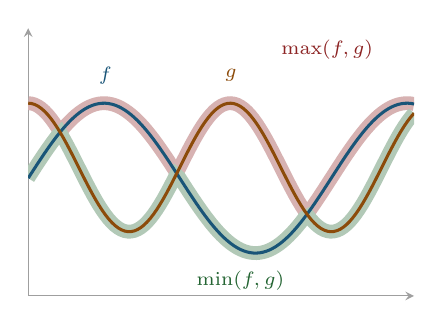
\begin{tikzpicture}
    \begin{axis}[swaxis, width=4.9cm, height=3.4cm, xmin=0, xmax=4, ymin=0, ymax=1.25,
        xtick=\empty, ytick=\empty, samples=121, domain=0:4]
      \addplot[thmcolor!35, line width=5pt] {max(0.55+0.35*sin(deg(2*x)), 0.6+0.3*cos(deg(3*x)))};
      \addplot[proofcolor!35, line width=5pt] {min(0.55+0.35*sin(deg(2*x)), 0.6+0.3*cos(deg(3*x)))};
      \addplot[defcolor, line width=1.1pt] {0.55+0.35*sin(deg(2*x))};
      \addplot[excolor, line width=1.1pt] {0.6+0.3*cos(deg(3*x))};
      \node[defcolor, font=\scriptsize] at (axis cs:0.8,1.03) {$f$};
      \node[excolor, font=\scriptsize] at (axis cs:2.1,1.03) {$g$};
      \node[thmcolor, font=\scriptsize] at (axis cs:3.1,1.15) {$\max(f,g)$};
      \node[proofcolor, font=\scriptsize] at (axis cs:2.2,0.07) {$\min(f,g)$};
    \end{axis}
  \end{tikzpicture}
    \end{column}
  \end{columns}

  \note{
    By iteration, the result extends to any finite collection. The maximum
    of three functions is the maximum of the first with the maximum of the
    other two, and so on. So capital "B" contains the maximum and the
    minimum of any finitely many of its members. Finiteness is essential
    here, and it is exactly what compactness will supply in the next two
    steps.
  }
\end{frame}

\begin{frame}{Proof of Theorem 7.32 --- Step 3}
  \begin{proofblock}{Step 3 (claim)}
    Given a real function $f$, continuous on $K$, a point $x \in K$, and $\varepsilon > 0$,
    there exists a function $g_x \in \mathscr{B}$ such that $g_x(x) = f(x)$ and
    \[
      g_x(t) > f(t) - \varepsilon \qquad (t \in K). \tag{54}
    \]
  \end{proofblock}

  \begin{center}
  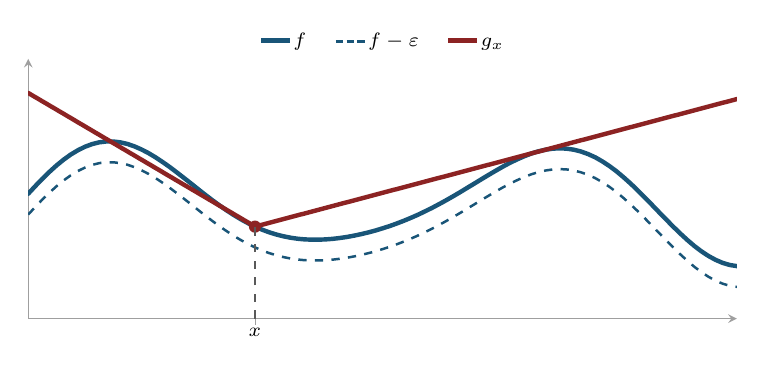
\begin{tikzpicture}
    \begin{axis}[swaxis, width=9cm, height=3.3cm, xmin=0, xmax=5, ymin=0.25, ymax=3.0,
        xtick={1.60}, xticklabels={$x$}, title={\scriptsize \textcolor{defcolor}{\rule[0.45ex]{1.3em}{1.6pt}}\,$f$ \quad \textcolor{defcolor}{\rule[0.45ex]{0.32em}{0.9pt}\,\rule[0.45ex]{0.32em}{0.9pt}\,\rule[0.45ex]{0.32em}{0.9pt}}\,$f - \varepsilon$ \quad \textcolor{thmcolor}{\rule[0.45ex]{1.3em}{1.6pt}}\,$g_x$}, title style={yshift=-1.2ex, fill=white, fill opacity=0.6, text opacity=1, inner sep=2pt}, ytick=\empty]
      \addplot[defcolor, dashed, line width=0.9pt] coordinates {(0.000,1.352) (0.050,1.433) (0.100,1.511) (0.150,1.584) (0.200,1.652) (0.250,1.713) (0.300,1.767) (0.350,1.812) (0.400,1.849) (0.450,1.877) (0.500,1.896) (0.550,1.905) (0.600,1.905) (0.650,1.896) (0.700,1.879) (0.750,1.853) (0.800,1.820) (0.850,1.781) (0.900,1.736) (0.950,1.686) (1.000,1.633) (1.050,1.576) (1.100,1.518) (1.150,1.459) (1.200,1.399) (1.250,1.340) (1.300,1.283) (1.350,1.228) (1.400,1.176) (1.450,1.127) (1.500,1.082) (1.550,1.041) (1.600,1.004) (1.650,0.972) (1.700,0.944) (1.750,0.921) (1.800,0.902) (1.850,0.887) (1.900,0.876) (1.950,0.869) (2.000,0.866) (2.050,0.866) (2.100,0.869) (2.150,0.875) (2.200,0.884) (2.250,0.895) (2.300,0.909) (2.350,0.925) (2.400,0.943) (2.450,0.963) (2.500,0.986) (2.550,1.010) (2.600,1.037) (2.650,1.066) (2.700,1.097) (2.750,1.130) (2.800,1.166) (2.850,1.203) (2.900,1.243) (2.950,1.284) (3.000,1.327) (3.050,1.371) (3.100,1.417) (3.150,1.462) (3.200,1.508) (3.250,1.553) (3.300,1.597) (3.350,1.640) (3.400,1.680) (3.450,1.716) (3.500,1.749) (3.550,1.778) (3.600,1.801) (3.650,1.818) (3.700,1.829) (3.750,1.833) (3.800,1.829) (3.850,1.818) (3.900,1.799) (3.950,1.772) (4.000,1.738) (4.050,1.695) (4.100,1.646) (4.150,1.590) (4.200,1.527) (4.250,1.460) (4.300,1.388) (4.350,1.313) (4.400,1.236) (4.450,1.158) (4.500,1.081) (4.550,1.005) (4.600,0.932) (4.650,0.863) (4.700,0.799) (4.750,0.742) (4.800,0.693) (4.850,0.652) (4.900,0.620) (4.950,0.598) (5.000,0.586)};
      \addplot[defcolor, curveln] coordinates {(0.000,1.572) (0.050,1.653) (0.100,1.731) (0.150,1.804) (0.200,1.872) (0.250,1.933) (0.300,1.987) (0.350,2.032) (0.400,2.069) (0.450,2.097) (0.500,2.116) (0.550,2.125) (0.600,2.125) (0.650,2.116) (0.700,2.099) (0.750,2.073) (0.800,2.040) (0.850,2.001) (0.900,1.956) (0.950,1.906) (1.000,1.853) (1.050,1.796) (1.100,1.738) (1.150,1.679) (1.200,1.619) (1.250,1.560) (1.300,1.503) (1.350,1.448) (1.400,1.396) (1.450,1.347) (1.500,1.302) (1.550,1.261) (1.600,1.224) (1.650,1.192) (1.700,1.164) (1.750,1.141) (1.800,1.122) (1.850,1.107) (1.900,1.096) (1.950,1.089) (2.000,1.086) (2.050,1.086) (2.100,1.089) (2.150,1.095) (2.200,1.104) (2.250,1.115) (2.300,1.129) (2.350,1.145) (2.400,1.163) (2.450,1.183) (2.500,1.206) (2.550,1.230) (2.600,1.257) (2.650,1.286) (2.700,1.317) (2.750,1.350) (2.800,1.386) (2.850,1.423) (2.900,1.463) (2.950,1.504) (3.000,1.547) (3.050,1.591) (3.100,1.637) (3.150,1.682) (3.200,1.728) (3.250,1.773) (3.300,1.817) (3.350,1.860) (3.400,1.900) (3.450,1.936) (3.500,1.969) (3.550,1.998) (3.600,2.021) (3.650,2.038) (3.700,2.049) (3.750,2.053) (3.800,2.049) (3.850,2.038) (3.900,2.019) (3.950,1.992) (4.000,1.958) (4.050,1.915) (4.100,1.866) (4.150,1.810) (4.200,1.747) (4.250,1.680) (4.300,1.608) (4.350,1.533) (4.400,1.456) (4.450,1.378) (4.500,1.301) (4.550,1.225) (4.600,1.152) (4.650,1.083) (4.700,1.019) (4.750,0.962) (4.800,0.913) (4.850,0.872) (4.900,0.840) (4.950,0.818) (5.000,0.806)};
      \addplot[thmcolor, curveln] coordinates {(0.000,2.639) (0.020,2.621) (0.040,2.603) (0.060,2.586) (0.080,2.568) (0.100,2.550) (0.120,2.533) (0.140,2.515) (0.160,2.497) (0.180,2.480) (0.200,2.462) (0.220,2.444) (0.240,2.427) (0.260,2.409) (0.280,2.391) (0.300,2.374) (0.320,2.356) (0.340,2.338) (0.360,2.320) (0.380,2.303) (0.400,2.285) (0.420,2.267) (0.440,2.250) (0.460,2.232) (0.480,2.214) (0.500,2.197) (0.520,2.179) (0.540,2.161) (0.560,2.144) (0.580,2.126) (0.600,2.108) (0.620,2.091) (0.640,2.073) (0.660,2.055) (0.680,2.038) (0.700,2.020) (0.720,2.002) (0.740,1.985) (0.760,1.967) (0.780,1.949) (0.800,1.932) (0.820,1.914) (0.840,1.896) (0.860,1.879) (0.880,1.861) (0.900,1.843) (0.920,1.826) (0.940,1.808) (0.960,1.790) (0.980,1.772) (1.000,1.755) (1.020,1.737) (1.040,1.719) (1.060,1.702) (1.080,1.684) (1.100,1.666) (1.120,1.649) (1.140,1.631) (1.160,1.613) (1.180,1.596) (1.200,1.578) (1.220,1.560) (1.240,1.543) (1.260,1.525) (1.280,1.507) (1.300,1.490) (1.320,1.472) (1.340,1.454) (1.360,1.437) (1.380,1.419) (1.400,1.401) (1.420,1.384) (1.440,1.366) (1.460,1.348) (1.480,1.331) (1.500,1.313) (1.520,1.295) (1.540,1.278) (1.560,1.260) (1.580,1.242) (1.600,1.224) (1.620,1.232) (1.640,1.240) (1.660,1.248) (1.680,1.256) (1.700,1.264) (1.720,1.272) (1.740,1.280) (1.760,1.288) (1.780,1.296) (1.800,1.304) (1.820,1.312) (1.840,1.320) (1.860,1.328) (1.880,1.336) (1.900,1.344) (1.920,1.352) (1.940,1.359) (1.960,1.367) (1.980,1.375) (2.000,1.383) (2.020,1.391) (2.040,1.399) (2.060,1.407) (2.080,1.415) (2.100,1.423) (2.120,1.431) (2.140,1.439) (2.160,1.447) (2.180,1.455) (2.200,1.463) (2.220,1.471) (2.240,1.479) (2.260,1.486) (2.280,1.494) (2.300,1.502) (2.320,1.510) (2.340,1.518) (2.360,1.526) (2.380,1.534) (2.400,1.542) (2.420,1.550) (2.440,1.558) (2.460,1.566) (2.480,1.574) (2.500,1.582) (2.520,1.590) (2.540,1.598) (2.560,1.606) (2.580,1.614) (2.600,1.621) (2.620,1.629) (2.640,1.637) (2.660,1.645) (2.680,1.653) (2.700,1.661) (2.720,1.669) (2.740,1.677) (2.760,1.685) (2.780,1.693) (2.800,1.701) (2.820,1.709) (2.840,1.717) (2.860,1.725) (2.880,1.733) (2.900,1.741) (2.920,1.748) (2.940,1.756) (2.960,1.764) (2.980,1.772) (3.000,1.780) (3.020,1.788) (3.040,1.796) (3.060,1.804) (3.080,1.812) (3.100,1.820) (3.120,1.828) (3.140,1.836) (3.160,1.844) (3.180,1.852) (3.200,1.860) (3.220,1.868) (3.240,1.876) (3.260,1.883) (3.280,1.891) (3.300,1.899) (3.320,1.907) (3.340,1.915) (3.360,1.923) (3.380,1.931) (3.400,1.939) (3.420,1.947) (3.440,1.955) (3.460,1.963) (3.480,1.971) (3.500,1.979) (3.520,1.987) (3.540,1.995) (3.560,2.003) (3.580,2.011) (3.600,2.018) (3.620,2.026) (3.640,2.034) (3.660,2.042) (3.680,2.050) (3.700,2.058) (3.720,2.066) (3.740,2.074) (3.760,2.082) (3.780,2.090) (3.800,2.098) (3.820,2.106) (3.840,2.114) (3.860,2.122) (3.880,2.130) (3.900,2.138) (3.920,2.145) (3.940,2.153) (3.960,2.161) (3.980,2.169) (4.000,2.177) (4.020,2.185) (4.040,2.193) (4.060,2.201) (4.080,2.209) (4.100,2.217) (4.120,2.225) (4.140,2.233) (4.160,2.241) (4.180,2.249) (4.200,2.257) (4.220,2.265) (4.240,2.273) (4.260,2.280) (4.280,2.288) (4.300,2.296) (4.320,2.304) (4.340,2.312) (4.360,2.320) (4.380,2.328) (4.400,2.336) (4.420,2.344) (4.440,2.352) (4.460,2.360) (4.480,2.368) (4.500,2.376) (4.520,2.384) (4.540,2.392) (4.560,2.400) (4.580,2.407) (4.600,2.415) (4.620,2.423) (4.640,2.431) (4.660,2.439) (4.680,2.447) (4.700,2.455) (4.720,2.463) (4.740,2.471) (4.760,2.479) (4.780,2.487) (4.800,2.495) (4.820,2.503) (4.840,2.511) (4.860,2.519) (4.880,2.527) (4.900,2.535) (4.920,2.542) (4.940,2.550) (4.960,2.558) (4.980,2.566) (5.000,2.574)};
      \fill[thmcolor] (axis cs:1.60,1.224) circle (2.2pt);
      \draw[gray!70!black, dashed] (axis cs:1.60,0.25) -- (axis cs:1.60,1.224);
    \end{axis}
  \end{tikzpicture}
  \end{center}

  \note{
    Step 3 is the heart of the proof. Let "f" be a real continuous function
    on capital "K", fix a point "x" in capital "K", and let epsilon be
    given. The claim is that capital "B" contains a function "g" sub "x"
    that equals "f" at the point "x" and is greater than "f" minus epsilon
    at every point "t" of capital "K". That inequality is equation 54. The
    picture shows the goal, with capital "K" drawn as an interval. The
    legend above the plot identifies the curves. The solid blue curve is
    "f", and the dashed blue curve is "f" minus epsilon. The red curve is
    "g" sub "x". It touches the graph of "f" at the red dot above the point
    "x", and it never dips below the dashed curve. It is allowed to rise far
    above "f". We only control it from below. Let's construct it.
  }
\end{frame}

% --- Build 1/3 ---
\begin{frame}{Proof of Theorem 7.32 --- Step 3}
  \begin{columns}[T]
    \begin{column}{0.52\textwidth}
      \small
      \begin{proofblock}{Proof of Step 3}
        $\mathscr{A} \subset \mathscr{B}$, so Theorem 7.31 applies to $\mathscr{B}$:
        for every $y \in K$ there is $h_y \in \mathscr{B}$ with
        \[
          h_y(x) = f(x), \quad h_y(y) = f(y). \tag{55}
        \]
      \end{proofblock}
    \end{column}
    \begin{column}{0.46\textwidth}
      \centering
  \vspace{0.6em}
  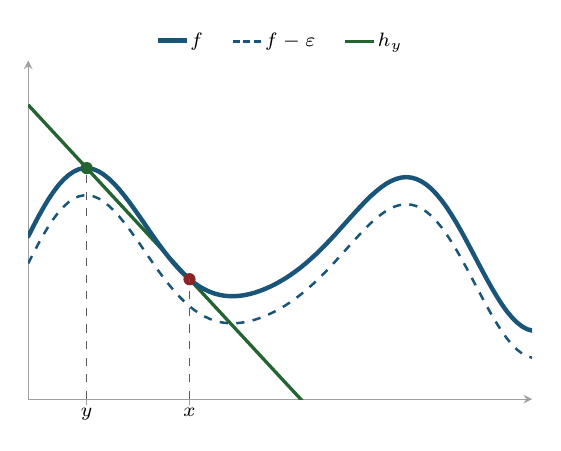
\begin{tikzpicture}
    \begin{axis}[swaxis, width=6.4cm, height=4.3cm, xmin=0, xmax=5, ymin=0.25, ymax=3.0,
        xtick={0.58,1.60}, xticklabels={$y$,$x$}, title={\scriptsize \textcolor{defcolor}{\rule[0.45ex]{1.3em}{1.6pt}}\,$f$ \quad \textcolor{defcolor}{\rule[0.45ex]{0.32em}{0.9pt}\,\rule[0.45ex]{0.32em}{0.9pt}\,\rule[0.45ex]{0.32em}{0.9pt}}\,$f - \varepsilon$ \quad \textcolor{proofcolor}{\rule[0.45ex]{1.3em}{1.2pt}}\,$h_y$}, title style={yshift=-1.2ex, fill=white, fill opacity=0.6, text opacity=1, inner sep=2pt}, ytick=\empty]
      \addplot[defcolor, dashed, line width=0.9pt] coordinates {(0.000,1.352) (0.050,1.433) (0.100,1.511) (0.150,1.584) (0.200,1.652) (0.250,1.713) (0.300,1.767) (0.350,1.812) (0.400,1.849) (0.450,1.877) (0.500,1.896) (0.550,1.905) (0.600,1.905) (0.650,1.896) (0.700,1.879) (0.750,1.853) (0.800,1.820) (0.850,1.781) (0.900,1.736) (0.950,1.686) (1.000,1.633) (1.050,1.576) (1.100,1.518) (1.150,1.459) (1.200,1.399) (1.250,1.340) (1.300,1.283) (1.350,1.228) (1.400,1.176) (1.450,1.127) (1.500,1.082) (1.550,1.041) (1.600,1.004) (1.650,0.972) (1.700,0.944) (1.750,0.921) (1.800,0.902) (1.850,0.887) (1.900,0.876) (1.950,0.869) (2.000,0.866) (2.050,0.866) (2.100,0.869) (2.150,0.875) (2.200,0.884) (2.250,0.895) (2.300,0.909) (2.350,0.925) (2.400,0.943) (2.450,0.963) (2.500,0.986) (2.550,1.010) (2.600,1.037) (2.650,1.066) (2.700,1.097) (2.750,1.130) (2.800,1.166) (2.850,1.203) (2.900,1.243) (2.950,1.284) (3.000,1.327) (3.050,1.371) (3.100,1.417) (3.150,1.462) (3.200,1.508) (3.250,1.553) (3.300,1.597) (3.350,1.640) (3.400,1.680) (3.450,1.716) (3.500,1.749) (3.550,1.778) (3.600,1.801) (3.650,1.818) (3.700,1.829) (3.750,1.833) (3.800,1.829) (3.850,1.818) (3.900,1.799) (3.950,1.772) (4.000,1.738) (4.050,1.695) (4.100,1.646) (4.150,1.590) (4.200,1.527) (4.250,1.460) (4.300,1.388) (4.350,1.313) (4.400,1.236) (4.450,1.158) (4.500,1.081) (4.550,1.005) (4.600,0.932) (4.650,0.863) (4.700,0.799) (4.750,0.742) (4.800,0.693) (4.850,0.652) (4.900,0.620) (4.950,0.598) (5.000,0.586)};
      \addplot[proofcolor, line width=1.2pt] coordinates {(0,2.639) (5,-1.781)};
      \addplot[defcolor, curveln] coordinates {(0.000,1.572) (0.050,1.653) (0.100,1.731) (0.150,1.804) (0.200,1.872) (0.250,1.933) (0.300,1.987) (0.350,2.032) (0.400,2.069) (0.450,2.097) (0.500,2.116) (0.550,2.125) (0.600,2.125) (0.650,2.116) (0.700,2.099) (0.750,2.073) (0.800,2.040) (0.850,2.001) (0.900,1.956) (0.950,1.906) (1.000,1.853) (1.050,1.796) (1.100,1.738) (1.150,1.679) (1.200,1.619) (1.250,1.560) (1.300,1.503) (1.350,1.448) (1.400,1.396) (1.450,1.347) (1.500,1.302) (1.550,1.261) (1.600,1.224) (1.650,1.192) (1.700,1.164) (1.750,1.141) (1.800,1.122) (1.850,1.107) (1.900,1.096) (1.950,1.089) (2.000,1.086) (2.050,1.086) (2.100,1.089) (2.150,1.095) (2.200,1.104) (2.250,1.115) (2.300,1.129) (2.350,1.145) (2.400,1.163) (2.450,1.183) (2.500,1.206) (2.550,1.230) (2.600,1.257) (2.650,1.286) (2.700,1.317) (2.750,1.350) (2.800,1.386) (2.850,1.423) (2.900,1.463) (2.950,1.504) (3.000,1.547) (3.050,1.591) (3.100,1.637) (3.150,1.682) (3.200,1.728) (3.250,1.773) (3.300,1.817) (3.350,1.860) (3.400,1.900) (3.450,1.936) (3.500,1.969) (3.550,1.998) (3.600,2.021) (3.650,2.038) (3.700,2.049) (3.750,2.053) (3.800,2.049) (3.850,2.038) (3.900,2.019) (3.950,1.992) (4.000,1.958) (4.050,1.915) (4.100,1.866) (4.150,1.810) (4.200,1.747) (4.250,1.680) (4.300,1.608) (4.350,1.533) (4.400,1.456) (4.450,1.378) (4.500,1.301) (4.550,1.225) (4.600,1.152) (4.650,1.083) (4.700,1.019) (4.750,0.962) (4.800,0.913) (4.850,0.872) (4.900,0.840) (4.950,0.818) (5.000,0.806)};
      \fill[thmcolor] (axis cs:1.60,1.224) circle (2.2pt);
      \draw[gray!70!black, dashed] (axis cs:1.60,0.25) -- (axis cs:1.60,1.224);
      \fill[proofcolor] (axis cs:0.58,2.126) circle (2.2pt);
      \draw[gray!70!black, dashed] (axis cs:0.58,0.25) -- (axis cs:0.58,2.126);
    \end{axis}
  \end{tikzpicture}
    \end{column}
  \end{columns}

  \note{
    Since capital "B" contains capital "A", it also separates points and
    vanishes at no point, so Theorem 7.31 applies to capital "B". For every
    point "y" of capital "K" it gives a function "h" sub "y" in capital "B"
    that agrees with "f" at the two points "x" and "y". This is equation 55.
    If "y" happens to equal "x", only one condition is needed. In the
    picture, the algebra consists of polynomials, and "h" sub "y" is the
    green straight line through the red dot above "x" and the green dot
    above "y", both on the graph of "f".
  }
\end{frame}

% --- Build 2/3 ---
\begin{frame}{Proof of Theorem 7.32 --- Step 3}
  \begin{columns}[T]
    \begin{column}{0.52\textwidth}
      \small
      \begin{proofblock}{Proof of Step 3}
        $\mathscr{A} \subset \mathscr{B}$, so Theorem 7.31 applies to $\mathscr{B}$:
        for every $y \in K$ there is $h_y \in \mathscr{B}$ with
        \[
          h_y(x) = f(x), \quad h_y(y) = f(y). \tag{55}
        \]
        $h_y$ is continuous: there is an open $J_y \ni y$ with
        \[
          h_y(t) > f(t) - \varepsilon \quad (t \in J_y). \tag{56}
        \]
      \end{proofblock}
    \end{column}
    \begin{column}{0.46\textwidth}
      \centering
  \vspace{0.6em}
  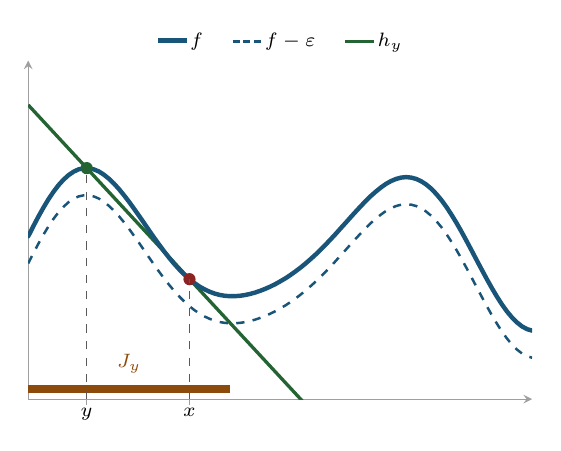
\begin{tikzpicture}
    \begin{axis}[swaxis, width=6.4cm, height=4.3cm, xmin=0, xmax=5, ymin=0.25, ymax=3.0,
        xtick={0.58,1.60}, xticklabels={$y$,$x$}, title={\scriptsize \textcolor{defcolor}{\rule[0.45ex]{1.3em}{1.6pt}}\,$f$ \quad \textcolor{defcolor}{\rule[0.45ex]{0.32em}{0.9pt}\,\rule[0.45ex]{0.32em}{0.9pt}\,\rule[0.45ex]{0.32em}{0.9pt}}\,$f - \varepsilon$ \quad \textcolor{proofcolor}{\rule[0.45ex]{1.3em}{1.2pt}}\,$h_y$}, title style={yshift=-1.2ex, fill=white, fill opacity=0.6, text opacity=1, inner sep=2pt}, ytick=\empty]
      \addplot[defcolor, dashed, line width=0.9pt] coordinates {(0.000,1.352) (0.050,1.433) (0.100,1.511) (0.150,1.584) (0.200,1.652) (0.250,1.713) (0.300,1.767) (0.350,1.812) (0.400,1.849) (0.450,1.877) (0.500,1.896) (0.550,1.905) (0.600,1.905) (0.650,1.896) (0.700,1.879) (0.750,1.853) (0.800,1.820) (0.850,1.781) (0.900,1.736) (0.950,1.686) (1.000,1.633) (1.050,1.576) (1.100,1.518) (1.150,1.459) (1.200,1.399) (1.250,1.340) (1.300,1.283) (1.350,1.228) (1.400,1.176) (1.450,1.127) (1.500,1.082) (1.550,1.041) (1.600,1.004) (1.650,0.972) (1.700,0.944) (1.750,0.921) (1.800,0.902) (1.850,0.887) (1.900,0.876) (1.950,0.869) (2.000,0.866) (2.050,0.866) (2.100,0.869) (2.150,0.875) (2.200,0.884) (2.250,0.895) (2.300,0.909) (2.350,0.925) (2.400,0.943) (2.450,0.963) (2.500,0.986) (2.550,1.010) (2.600,1.037) (2.650,1.066) (2.700,1.097) (2.750,1.130) (2.800,1.166) (2.850,1.203) (2.900,1.243) (2.950,1.284) (3.000,1.327) (3.050,1.371) (3.100,1.417) (3.150,1.462) (3.200,1.508) (3.250,1.553) (3.300,1.597) (3.350,1.640) (3.400,1.680) (3.450,1.716) (3.500,1.749) (3.550,1.778) (3.600,1.801) (3.650,1.818) (3.700,1.829) (3.750,1.833) (3.800,1.829) (3.850,1.818) (3.900,1.799) (3.950,1.772) (4.000,1.738) (4.050,1.695) (4.100,1.646) (4.150,1.590) (4.200,1.527) (4.250,1.460) (4.300,1.388) (4.350,1.313) (4.400,1.236) (4.450,1.158) (4.500,1.081) (4.550,1.005) (4.600,0.932) (4.650,0.863) (4.700,0.799) (4.750,0.742) (4.800,0.693) (4.850,0.652) (4.900,0.620) (4.950,0.598) (5.000,0.586)};
      \addplot[proofcolor, line width=1.2pt] coordinates {(0,2.639) (5,-1.781)};
      \draw[excolor, line width=3pt] (axis cs:0.000,0.33) -- (axis cs:2.000,0.33);
      \node[excolor, font=\scriptsize, anchor=south] at (axis cs:1.00,0.38) {$J_y$};
      \addplot[defcolor, curveln] coordinates {(0.000,1.572) (0.050,1.653) (0.100,1.731) (0.150,1.804) (0.200,1.872) (0.250,1.933) (0.300,1.987) (0.350,2.032) (0.400,2.069) (0.450,2.097) (0.500,2.116) (0.550,2.125) (0.600,2.125) (0.650,2.116) (0.700,2.099) (0.750,2.073) (0.800,2.040) (0.850,2.001) (0.900,1.956) (0.950,1.906) (1.000,1.853) (1.050,1.796) (1.100,1.738) (1.150,1.679) (1.200,1.619) (1.250,1.560) (1.300,1.503) (1.350,1.448) (1.400,1.396) (1.450,1.347) (1.500,1.302) (1.550,1.261) (1.600,1.224) (1.650,1.192) (1.700,1.164) (1.750,1.141) (1.800,1.122) (1.850,1.107) (1.900,1.096) (1.950,1.089) (2.000,1.086) (2.050,1.086) (2.100,1.089) (2.150,1.095) (2.200,1.104) (2.250,1.115) (2.300,1.129) (2.350,1.145) (2.400,1.163) (2.450,1.183) (2.500,1.206) (2.550,1.230) (2.600,1.257) (2.650,1.286) (2.700,1.317) (2.750,1.350) (2.800,1.386) (2.850,1.423) (2.900,1.463) (2.950,1.504) (3.000,1.547) (3.050,1.591) (3.100,1.637) (3.150,1.682) (3.200,1.728) (3.250,1.773) (3.300,1.817) (3.350,1.860) (3.400,1.900) (3.450,1.936) (3.500,1.969) (3.550,1.998) (3.600,2.021) (3.650,2.038) (3.700,2.049) (3.750,2.053) (3.800,2.049) (3.850,2.038) (3.900,2.019) (3.950,1.992) (4.000,1.958) (4.050,1.915) (4.100,1.866) (4.150,1.810) (4.200,1.747) (4.250,1.680) (4.300,1.608) (4.350,1.533) (4.400,1.456) (4.450,1.378) (4.500,1.301) (4.550,1.225) (4.600,1.152) (4.650,1.083) (4.700,1.019) (4.750,0.962) (4.800,0.913) (4.850,0.872) (4.900,0.840) (4.950,0.818) (5.000,0.806)};
      \fill[thmcolor] (axis cs:1.60,1.224) circle (2.2pt);
      \draw[gray!70!black, dashed] (axis cs:1.60,0.25) -- (axis cs:1.60,1.224);
      \fill[proofcolor] (axis cs:0.58,2.126) circle (2.2pt);
      \draw[gray!70!black, dashed] (axis cs:0.58,0.25) -- (axis cs:0.58,2.126);
    \end{axis}
  \end{tikzpicture}
    \end{column}
  \end{columns}

  \note{
    At the point "y" itself, "h" sub "y" equals "f", so it is strictly above
    "f" minus epsilon there. Both functions are continuous, so this strict
    inequality persists on a whole open set containing "y", called capital
    "J" sub "y". This is equation 56. In the picture, capital "J" sub "y" is
    the thick amber part of the horizontal axis: the set of points where the
    green line lies above the dashed curve. It contains "y", and also "x".
    Outside it, the line falls below the dashed curve, so one line is not
    enough.
  }
\end{frame}

% --- Build 3/3 ---
\begin{frame}{Proof of Theorem 7.32 --- Step 3}
  \begin{columns}[T]
    \begin{column}{0.52\textwidth}
      \small
      \begin{proofblock}{Proof of Step 3}
        $\mathscr{A} \subset \mathscr{B}$, so Theorem 7.31 applies to $\mathscr{B}$:
        for every $y \in K$ there is $h_y \in \mathscr{B}$ with
        \[
          h_y(x) = f(x), \quad h_y(y) = f(y). \tag{55}
        \]
        $h_y$ is continuous: there is an open $J_y \ni y$ with
        \[
          h_y(t) > f(t) - \varepsilon \quad (t \in J_y). \tag{56}
        \]
        $K$ is compact: there are $y_1, \dots, y_n$ with
        \[
          K \subset J_{y_1} \cup \cdots \cup J_{y_n}. \tag{57}
        \]
        Put $g_x = \max(h_{y_1}, \dots, h_{y_n}) \in \mathscr{B}$ (Step 2).\\
        (55)--(57) give the rest. \hfill $\blacksquare$
      \end{proofblock}
    \end{column}
    \begin{column}{0.46\textwidth}
      \centering
  \vspace{0.6em}
  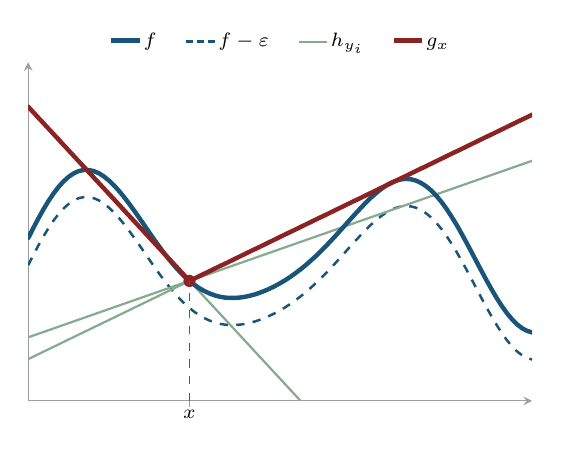
\begin{tikzpicture}
    \begin{axis}[swaxis, width=6.4cm, height=4.3cm, xmin=0, xmax=5, ymin=0.25, ymax=3.0,
        xtick={1.60}, xticklabels={$x$}, title={\scriptsize \textcolor{defcolor}{\rule[0.45ex]{1.3em}{1.6pt}}\,$f$ \quad \textcolor{defcolor}{\rule[0.45ex]{0.32em}{0.9pt}\,\rule[0.45ex]{0.32em}{0.9pt}\,\rule[0.45ex]{0.32em}{0.9pt}}\,$f - \varepsilon$ \quad \textcolor{proofcolor!55}{\rule[0.45ex]{1.3em}{0.8pt}}\,$h_{y_i}$ \quad \textcolor{thmcolor}{\rule[0.45ex]{1.3em}{1.6pt}}\,$g_x$}, title style={yshift=-1.2ex, fill=white, fill opacity=0.6, text opacity=1, inner sep=2pt}, ytick=\empty]
      \addplot[defcolor, dashed, line width=0.9pt] coordinates {(0.000,1.352) (0.050,1.433) (0.100,1.511) (0.150,1.584) (0.200,1.652) (0.250,1.713) (0.300,1.767) (0.350,1.812) (0.400,1.849) (0.450,1.877) (0.500,1.896) (0.550,1.905) (0.600,1.905) (0.650,1.896) (0.700,1.879) (0.750,1.853) (0.800,1.820) (0.850,1.781) (0.900,1.736) (0.950,1.686) (1.000,1.633) (1.050,1.576) (1.100,1.518) (1.150,1.459) (1.200,1.399) (1.250,1.340) (1.300,1.283) (1.350,1.228) (1.400,1.176) (1.450,1.127) (1.500,1.082) (1.550,1.041) (1.600,1.004) (1.650,0.972) (1.700,0.944) (1.750,0.921) (1.800,0.902) (1.850,0.887) (1.900,0.876) (1.950,0.869) (2.000,0.866) (2.050,0.866) (2.100,0.869) (2.150,0.875) (2.200,0.884) (2.250,0.895) (2.300,0.909) (2.350,0.925) (2.400,0.943) (2.450,0.963) (2.500,0.986) (2.550,1.010) (2.600,1.037) (2.650,1.066) (2.700,1.097) (2.750,1.130) (2.800,1.166) (2.850,1.203) (2.900,1.243) (2.950,1.284) (3.000,1.327) (3.050,1.371) (3.100,1.417) (3.150,1.462) (3.200,1.508) (3.250,1.553) (3.300,1.597) (3.350,1.640) (3.400,1.680) (3.450,1.716) (3.500,1.749) (3.550,1.778) (3.600,1.801) (3.650,1.818) (3.700,1.829) (3.750,1.833) (3.800,1.829) (3.850,1.818) (3.900,1.799) (3.950,1.772) (4.000,1.738) (4.050,1.695) (4.100,1.646) (4.150,1.590) (4.200,1.527) (4.250,1.460) (4.300,1.388) (4.350,1.313) (4.400,1.236) (4.450,1.158) (4.500,1.081) (4.550,1.005) (4.600,0.932) (4.650,0.863) (4.700,0.799) (4.750,0.742) (4.800,0.693) (4.850,0.652) (4.900,0.620) (4.950,0.598) (5.000,0.586)};
      \addplot[proofcolor!55, line width=0.8pt] coordinates {(0,2.639) (5,-1.781)};
      \addplot[proofcolor!55, line width=0.8pt] coordinates {(0,0.766) (5,2.200)};
      \addplot[proofcolor!55, line width=0.8pt] coordinates {(0,0.589) (5,2.574)};
      \addplot[defcolor, curveln] coordinates {(0.000,1.572) (0.050,1.653) (0.100,1.731) (0.150,1.804) (0.200,1.872) (0.250,1.933) (0.300,1.987) (0.350,2.032) (0.400,2.069) (0.450,2.097) (0.500,2.116) (0.550,2.125) (0.600,2.125) (0.650,2.116) (0.700,2.099) (0.750,2.073) (0.800,2.040) (0.850,2.001) (0.900,1.956) (0.950,1.906) (1.000,1.853) (1.050,1.796) (1.100,1.738) (1.150,1.679) (1.200,1.619) (1.250,1.560) (1.300,1.503) (1.350,1.448) (1.400,1.396) (1.450,1.347) (1.500,1.302) (1.550,1.261) (1.600,1.224) (1.650,1.192) (1.700,1.164) (1.750,1.141) (1.800,1.122) (1.850,1.107) (1.900,1.096) (1.950,1.089) (2.000,1.086) (2.050,1.086) (2.100,1.089) (2.150,1.095) (2.200,1.104) (2.250,1.115) (2.300,1.129) (2.350,1.145) (2.400,1.163) (2.450,1.183) (2.500,1.206) (2.550,1.230) (2.600,1.257) (2.650,1.286) (2.700,1.317) (2.750,1.350) (2.800,1.386) (2.850,1.423) (2.900,1.463) (2.950,1.504) (3.000,1.547) (3.050,1.591) (3.100,1.637) (3.150,1.682) (3.200,1.728) (3.250,1.773) (3.300,1.817) (3.350,1.860) (3.400,1.900) (3.450,1.936) (3.500,1.969) (3.550,1.998) (3.600,2.021) (3.650,2.038) (3.700,2.049) (3.750,2.053) (3.800,2.049) (3.850,2.038) (3.900,2.019) (3.950,1.992) (4.000,1.958) (4.050,1.915) (4.100,1.866) (4.150,1.810) (4.200,1.747) (4.250,1.680) (4.300,1.608) (4.350,1.533) (4.400,1.456) (4.450,1.378) (4.500,1.301) (4.550,1.225) (4.600,1.152) (4.650,1.083) (4.700,1.019) (4.750,0.962) (4.800,0.913) (4.850,0.872) (4.900,0.840) (4.950,0.818) (5.000,0.806)};
      \addplot[thmcolor, curveln] coordinates {(0.000,2.639) (0.020,2.621) (0.040,2.603) (0.060,2.586) (0.080,2.568) (0.100,2.550) (0.120,2.533) (0.140,2.515) (0.160,2.497) (0.180,2.480) (0.200,2.462) (0.220,2.444) (0.240,2.427) (0.260,2.409) (0.280,2.391) (0.300,2.374) (0.320,2.356) (0.340,2.338) (0.360,2.320) (0.380,2.303) (0.400,2.285) (0.420,2.267) (0.440,2.250) (0.460,2.232) (0.480,2.214) (0.500,2.197) (0.520,2.179) (0.540,2.161) (0.560,2.144) (0.580,2.126) (0.600,2.108) (0.620,2.091) (0.640,2.073) (0.660,2.055) (0.680,2.038) (0.700,2.020) (0.720,2.002) (0.740,1.985) (0.760,1.967) (0.780,1.949) (0.800,1.932) (0.820,1.914) (0.840,1.896) (0.860,1.879) (0.880,1.861) (0.900,1.843) (0.920,1.826) (0.940,1.808) (0.960,1.790) (0.980,1.772) (1.000,1.755) (1.020,1.737) (1.040,1.719) (1.060,1.702) (1.080,1.684) (1.100,1.666) (1.120,1.649) (1.140,1.631) (1.160,1.613) (1.180,1.596) (1.200,1.578) (1.220,1.560) (1.240,1.543) (1.260,1.525) (1.280,1.507) (1.300,1.490) (1.320,1.472) (1.340,1.454) (1.360,1.437) (1.380,1.419) (1.400,1.401) (1.420,1.384) (1.440,1.366) (1.460,1.348) (1.480,1.331) (1.500,1.313) (1.520,1.295) (1.540,1.278) (1.560,1.260) (1.580,1.242) (1.600,1.224) (1.620,1.232) (1.640,1.240) (1.660,1.248) (1.680,1.256) (1.700,1.264) (1.720,1.272) (1.740,1.280) (1.760,1.288) (1.780,1.296) (1.800,1.304) (1.820,1.312) (1.840,1.320) (1.860,1.328) (1.880,1.336) (1.900,1.344) (1.920,1.352) (1.940,1.359) (1.960,1.367) (1.980,1.375) (2.000,1.383) (2.020,1.391) (2.040,1.399) (2.060,1.407) (2.080,1.415) (2.100,1.423) (2.120,1.431) (2.140,1.439) (2.160,1.447) (2.180,1.455) (2.200,1.463) (2.220,1.471) (2.240,1.479) (2.260,1.486) (2.280,1.494) (2.300,1.502) (2.320,1.510) (2.340,1.518) (2.360,1.526) (2.380,1.534) (2.400,1.542) (2.420,1.550) (2.440,1.558) (2.460,1.566) (2.480,1.574) (2.500,1.582) (2.520,1.590) (2.540,1.598) (2.560,1.606) (2.580,1.614) (2.600,1.621) (2.620,1.629) (2.640,1.637) (2.660,1.645) (2.680,1.653) (2.700,1.661) (2.720,1.669) (2.740,1.677) (2.760,1.685) (2.780,1.693) (2.800,1.701) (2.820,1.709) (2.840,1.717) (2.860,1.725) (2.880,1.733) (2.900,1.741) (2.920,1.748) (2.940,1.756) (2.960,1.764) (2.980,1.772) (3.000,1.780) (3.020,1.788) (3.040,1.796) (3.060,1.804) (3.080,1.812) (3.100,1.820) (3.120,1.828) (3.140,1.836) (3.160,1.844) (3.180,1.852) (3.200,1.860) (3.220,1.868) (3.240,1.876) (3.260,1.883) (3.280,1.891) (3.300,1.899) (3.320,1.907) (3.340,1.915) (3.360,1.923) (3.380,1.931) (3.400,1.939) (3.420,1.947) (3.440,1.955) (3.460,1.963) (3.480,1.971) (3.500,1.979) (3.520,1.987) (3.540,1.995) (3.560,2.003) (3.580,2.011) (3.600,2.018) (3.620,2.026) (3.640,2.034) (3.660,2.042) (3.680,2.050) (3.700,2.058) (3.720,2.066) (3.740,2.074) (3.760,2.082) (3.780,2.090) (3.800,2.098) (3.820,2.106) (3.840,2.114) (3.860,2.122) (3.880,2.130) (3.900,2.138) (3.920,2.145) (3.940,2.153) (3.960,2.161) (3.980,2.169) (4.000,2.177) (4.020,2.185) (4.040,2.193) (4.060,2.201) (4.080,2.209) (4.100,2.217) (4.120,2.225) (4.140,2.233) (4.160,2.241) (4.180,2.249) (4.200,2.257) (4.220,2.265) (4.240,2.273) (4.260,2.280) (4.280,2.288) (4.300,2.296) (4.320,2.304) (4.340,2.312) (4.360,2.320) (4.380,2.328) (4.400,2.336) (4.420,2.344) (4.440,2.352) (4.460,2.360) (4.480,2.368) (4.500,2.376) (4.520,2.384) (4.540,2.392) (4.560,2.400) (4.580,2.407) (4.600,2.415) (4.620,2.423) (4.640,2.431) (4.660,2.439) (4.680,2.447) (4.700,2.455) (4.720,2.463) (4.740,2.471) (4.760,2.479) (4.780,2.487) (4.800,2.495) (4.820,2.503) (4.840,2.511) (4.860,2.519) (4.880,2.527) (4.900,2.535) (4.920,2.542) (4.940,2.550) (4.960,2.558) (4.980,2.566) (5.000,2.574)};
      \fill[thmcolor] (axis cs:1.60,1.224) circle (2.2pt);
      \draw[gray!70!black, dashed] (axis cs:1.60,0.25) -- (axis cs:1.60,1.224);
    \end{axis}
  \end{tikzpicture}
    \end{column}
  \end{columns}

  \note{
    As "y" ranges over capital "K", the open sets capital "J" sub "y" cover
    capital "K". By compactness, finitely many of them suffice, which is
    equation 57. Let "g" sub "x" be the maximum of the corresponding
    finitely many functions. By Step 2 it lies in capital "B". Each of them
    equals "f" at "x", so the maximum does too. And every point "t" lies in
    one of the sets, where the corresponding function already exceeds "f"
    minus epsilon, so the maximum does as well. In the picture, the thin
    green lines all pass through the red dot, and their upper envelope,
    drawn in red, stays above the dashed curve everywhere.
  }
\end{frame}

\begin{frame}{Proof of Theorem 7.32 --- Step 4}
  \begin{proofblock}{Step 4 (claim)}
    Given a real function $f$, continuous on $K$, and $\varepsilon > 0$, there exists a function
    $h \in \mathscr{B}$ such that
    \[
      |h(x) - f(x)| < \varepsilon \qquad (x \in K). \tag{58}
    \]
  \end{proofblock}
  \hl{\small Since $\mathscr{B}$ is uniformly closed, this is equivalent to the conclusion of the theorem.}

  \vspace{-0.4em}
  \begin{center}
  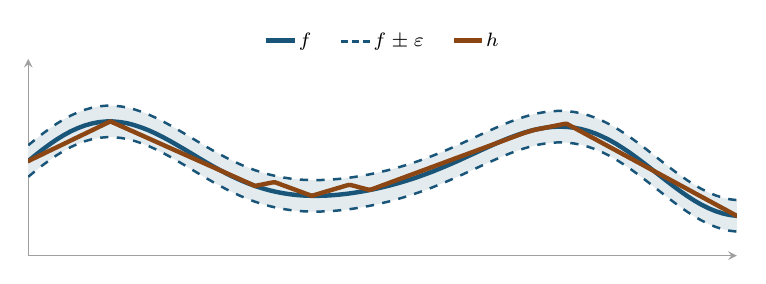
\begin{tikzpicture}
    \begin{axis}[swaxis, width=9cm, height=2.5cm, xmin=0, xmax=5, ymin=0.25, ymax=3.0,
        xtick=\empty, title={\scriptsize \textcolor{defcolor}{\rule[0.45ex]{1.3em}{1.6pt}}\,$f$ \quad \textcolor{defcolor}{\rule[0.45ex]{0.32em}{0.9pt}\,\rule[0.45ex]{0.32em}{0.9pt}\,\rule[0.45ex]{0.32em}{0.9pt}}\,$f \pm \varepsilon$ \quad \textcolor{mAccent}{\rule[0.45ex]{1.3em}{1.6pt}}\,$h$}, title style={yshift=-1.2ex, fill=white, fill opacity=0.6, text opacity=1, inner sep=2pt}, ytick=\empty]
      \addplot[draw=none, fill=defcolor!12] coordinates {(0.000,1.792) (0.050,1.873) (0.100,1.951) (0.150,2.024) (0.200,2.092) (0.250,2.153) (0.300,2.207) (0.350,2.252) (0.400,2.289) (0.450,2.317) (0.500,2.336) (0.550,2.345) (0.600,2.345) (0.650,2.336) (0.700,2.319) (0.750,2.293) (0.800,2.260) (0.850,2.221) (0.900,2.176) (0.950,2.126) (1.000,2.073) (1.050,2.016) (1.100,1.958) (1.150,1.899) (1.200,1.839) (1.250,1.780) (1.300,1.723) (1.350,1.668) (1.400,1.616) (1.450,1.567) (1.500,1.522) (1.550,1.481) (1.600,1.444) (1.650,1.412) (1.700,1.384) (1.750,1.361) (1.800,1.342) (1.850,1.327) (1.900,1.316) (1.950,1.309) (2.000,1.306) (2.050,1.306) (2.100,1.309) (2.150,1.315) (2.200,1.324) (2.250,1.335) (2.300,1.349) (2.350,1.365) (2.400,1.383) (2.450,1.403) (2.500,1.426) (2.550,1.450) (2.600,1.477) (2.650,1.506) (2.700,1.537) (2.750,1.570) (2.800,1.606) (2.850,1.643) (2.900,1.683) (2.950,1.724) (3.000,1.767) (3.050,1.811) (3.100,1.857) (3.150,1.902) (3.200,1.948) (3.250,1.993) (3.300,2.037) (3.350,2.080) (3.400,2.120) (3.450,2.156) (3.500,2.189) (3.550,2.218) (3.600,2.241) (3.650,2.258) (3.700,2.269) (3.750,2.273) (3.800,2.269) (3.850,2.258) (3.900,2.239) (3.950,2.212) (4.000,2.178) (4.050,2.135) (4.100,2.086) (4.150,2.030) (4.200,1.967) (4.250,1.900) (4.300,1.828) (4.350,1.753) (4.400,1.676) (4.450,1.598) (4.500,1.521) (4.550,1.445) (4.600,1.372) (4.650,1.303) (4.700,1.239) (4.750,1.182) (4.800,1.133) (4.850,1.092) (4.900,1.060) (4.950,1.038) (5.000,1.026) (5.000,0.586) (4.950,0.598) (4.900,0.620) (4.850,0.652) (4.800,0.693) (4.750,0.742) (4.700,0.799) (4.650,0.863) (4.600,0.932) (4.550,1.005) (4.500,1.081) (4.450,1.158) (4.400,1.236) (4.350,1.313) (4.300,1.388) (4.250,1.460) (4.200,1.527) (4.150,1.590) (4.100,1.646) (4.050,1.695) (4.000,1.738) (3.950,1.772) (3.900,1.799) (3.850,1.818) (3.800,1.829) (3.750,1.833) (3.700,1.829) (3.650,1.818) (3.600,1.801) (3.550,1.778) (3.500,1.749) (3.450,1.716) (3.400,1.680) (3.350,1.640) (3.300,1.597) (3.250,1.553) (3.200,1.508) (3.150,1.462) (3.100,1.417) (3.050,1.371) (3.000,1.327) (2.950,1.284) (2.900,1.243) (2.850,1.203) (2.800,1.166) (2.750,1.130) (2.700,1.097) (2.650,1.066) (2.600,1.037) (2.550,1.010) (2.500,0.986) (2.450,0.963) (2.400,0.943) (2.350,0.925) (2.300,0.909) (2.250,0.895) (2.200,0.884) (2.150,0.875) (2.100,0.869) (2.050,0.866) (2.000,0.866) (1.950,0.869) (1.900,0.876) (1.850,0.887) (1.800,0.902) (1.750,0.921) (1.700,0.944) (1.650,0.972) (1.600,1.004) (1.550,1.041) (1.500,1.082) (1.450,1.127) (1.400,1.176) (1.350,1.228) (1.300,1.283) (1.250,1.340) (1.200,1.399) (1.150,1.459) (1.100,1.518) (1.050,1.576) (1.000,1.633) (0.950,1.686) (0.900,1.736) (0.850,1.781) (0.800,1.820) (0.750,1.853) (0.700,1.879) (0.650,1.896) (0.600,1.905) (0.550,1.905) (0.500,1.896) (0.450,1.877) (0.400,1.849) (0.350,1.812) (0.300,1.767) (0.250,1.713) (0.200,1.652) (0.150,1.584) (0.100,1.511) (0.050,1.433) (0.000,1.352)} -- cycle;
      \addplot[defcolor, dashed, line width=0.9pt] coordinates {(0.000,1.792) (0.050,1.873) (0.100,1.951) (0.150,2.024) (0.200,2.092) (0.250,2.153) (0.300,2.207) (0.350,2.252) (0.400,2.289) (0.450,2.317) (0.500,2.336) (0.550,2.345) (0.600,2.345) (0.650,2.336) (0.700,2.319) (0.750,2.293) (0.800,2.260) (0.850,2.221) (0.900,2.176) (0.950,2.126) (1.000,2.073) (1.050,2.016) (1.100,1.958) (1.150,1.899) (1.200,1.839) (1.250,1.780) (1.300,1.723) (1.350,1.668) (1.400,1.616) (1.450,1.567) (1.500,1.522) (1.550,1.481) (1.600,1.444) (1.650,1.412) (1.700,1.384) (1.750,1.361) (1.800,1.342) (1.850,1.327) (1.900,1.316) (1.950,1.309) (2.000,1.306) (2.050,1.306) (2.100,1.309) (2.150,1.315) (2.200,1.324) (2.250,1.335) (2.300,1.349) (2.350,1.365) (2.400,1.383) (2.450,1.403) (2.500,1.426) (2.550,1.450) (2.600,1.477) (2.650,1.506) (2.700,1.537) (2.750,1.570) (2.800,1.606) (2.850,1.643) (2.900,1.683) (2.950,1.724) (3.000,1.767) (3.050,1.811) (3.100,1.857) (3.150,1.902) (3.200,1.948) (3.250,1.993) (3.300,2.037) (3.350,2.080) (3.400,2.120) (3.450,2.156) (3.500,2.189) (3.550,2.218) (3.600,2.241) (3.650,2.258) (3.700,2.269) (3.750,2.273) (3.800,2.269) (3.850,2.258) (3.900,2.239) (3.950,2.212) (4.000,2.178) (4.050,2.135) (4.100,2.086) (4.150,2.030) (4.200,1.967) (4.250,1.900) (4.300,1.828) (4.350,1.753) (4.400,1.676) (4.450,1.598) (4.500,1.521) (4.550,1.445) (4.600,1.372) (4.650,1.303) (4.700,1.239) (4.750,1.182) (4.800,1.133) (4.850,1.092) (4.900,1.060) (4.950,1.038) (5.000,1.026)};
      \addplot[defcolor, dashed, line width=0.9pt] coordinates {(0.000,1.352) (0.050,1.433) (0.100,1.511) (0.150,1.584) (0.200,1.652) (0.250,1.713) (0.300,1.767) (0.350,1.812) (0.400,1.849) (0.450,1.877) (0.500,1.896) (0.550,1.905) (0.600,1.905) (0.650,1.896) (0.700,1.879) (0.750,1.853) (0.800,1.820) (0.850,1.781) (0.900,1.736) (0.950,1.686) (1.000,1.633) (1.050,1.576) (1.100,1.518) (1.150,1.459) (1.200,1.399) (1.250,1.340) (1.300,1.283) (1.350,1.228) (1.400,1.176) (1.450,1.127) (1.500,1.082) (1.550,1.041) (1.600,1.004) (1.650,0.972) (1.700,0.944) (1.750,0.921) (1.800,0.902) (1.850,0.887) (1.900,0.876) (1.950,0.869) (2.000,0.866) (2.050,0.866) (2.100,0.869) (2.150,0.875) (2.200,0.884) (2.250,0.895) (2.300,0.909) (2.350,0.925) (2.400,0.943) (2.450,0.963) (2.500,0.986) (2.550,1.010) (2.600,1.037) (2.650,1.066) (2.700,1.097) (2.750,1.130) (2.800,1.166) (2.850,1.203) (2.900,1.243) (2.950,1.284) (3.000,1.327) (3.050,1.371) (3.100,1.417) (3.150,1.462) (3.200,1.508) (3.250,1.553) (3.300,1.597) (3.350,1.640) (3.400,1.680) (3.450,1.716) (3.500,1.749) (3.550,1.778) (3.600,1.801) (3.650,1.818) (3.700,1.829) (3.750,1.833) (3.800,1.829) (3.850,1.818) (3.900,1.799) (3.950,1.772) (4.000,1.738) (4.050,1.695) (4.100,1.646) (4.150,1.590) (4.200,1.527) (4.250,1.460) (4.300,1.388) (4.350,1.313) (4.400,1.236) (4.450,1.158) (4.500,1.081) (4.550,1.005) (4.600,0.932) (4.650,0.863) (4.700,0.799) (4.750,0.742) (4.800,0.693) (4.850,0.652) (4.900,0.620) (4.950,0.598) (5.000,0.586)};
      \addplot[defcolor, curveln] coordinates {(0.000,1.572) (0.050,1.653) (0.100,1.731) (0.150,1.804) (0.200,1.872) (0.250,1.933) (0.300,1.987) (0.350,2.032) (0.400,2.069) (0.450,2.097) (0.500,2.116) (0.550,2.125) (0.600,2.125) (0.650,2.116) (0.700,2.099) (0.750,2.073) (0.800,2.040) (0.850,2.001) (0.900,1.956) (0.950,1.906) (1.000,1.853) (1.050,1.796) (1.100,1.738) (1.150,1.679) (1.200,1.619) (1.250,1.560) (1.300,1.503) (1.350,1.448) (1.400,1.396) (1.450,1.347) (1.500,1.302) (1.550,1.261) (1.600,1.224) (1.650,1.192) (1.700,1.164) (1.750,1.141) (1.800,1.122) (1.850,1.107) (1.900,1.096) (1.950,1.089) (2.000,1.086) (2.050,1.086) (2.100,1.089) (2.150,1.095) (2.200,1.104) (2.250,1.115) (2.300,1.129) (2.350,1.145) (2.400,1.163) (2.450,1.183) (2.500,1.206) (2.550,1.230) (2.600,1.257) (2.650,1.286) (2.700,1.317) (2.750,1.350) (2.800,1.386) (2.850,1.423) (2.900,1.463) (2.950,1.504) (3.000,1.547) (3.050,1.591) (3.100,1.637) (3.150,1.682) (3.200,1.728) (3.250,1.773) (3.300,1.817) (3.350,1.860) (3.400,1.900) (3.450,1.936) (3.500,1.969) (3.550,1.998) (3.600,2.021) (3.650,2.038) (3.700,2.049) (3.750,2.053) (3.800,2.049) (3.850,2.038) (3.900,2.019) (3.950,1.992) (4.000,1.958) (4.050,1.915) (4.100,1.866) (4.150,1.810) (4.200,1.747) (4.250,1.680) (4.300,1.608) (4.350,1.533) (4.400,1.456) (4.450,1.378) (4.500,1.301) (4.550,1.225) (4.600,1.152) (4.650,1.083) (4.700,1.019) (4.750,0.962) (4.800,0.913) (4.850,0.872) (4.900,0.840) (4.950,0.818) (5.000,0.806)};
      \addplot[mAccent, curveln] coordinates {(0.000,1.572) (0.020,1.591) (0.040,1.610) (0.060,1.629) (0.080,1.648) (0.100,1.667) (0.120,1.687) (0.140,1.706) (0.160,1.725) (0.180,1.744) (0.200,1.763) (0.220,1.782) (0.240,1.801) (0.260,1.820) (0.280,1.839) (0.300,1.859) (0.320,1.878) (0.340,1.897) (0.360,1.916) (0.380,1.935) (0.400,1.954) (0.420,1.973) (0.440,1.992) (0.460,2.011) (0.480,2.030) (0.500,2.050) (0.520,2.069) (0.540,2.088) (0.560,2.107) (0.580,2.126) (0.600,2.108) (0.620,2.091) (0.640,2.073) (0.660,2.055) (0.680,2.038) (0.700,2.020) (0.720,2.002) (0.740,1.985) (0.760,1.967) (0.780,1.949) (0.800,1.932) (0.820,1.914) (0.840,1.896) (0.860,1.879) (0.880,1.861) (0.900,1.843) (0.920,1.826) (0.940,1.808) (0.960,1.790) (0.980,1.772) (1.000,1.755) (1.020,1.737) (1.040,1.719) (1.060,1.702) (1.080,1.684) (1.100,1.666) (1.120,1.649) (1.140,1.631) (1.160,1.613) (1.180,1.596) (1.200,1.578) (1.220,1.560) (1.240,1.543) (1.260,1.525) (1.280,1.507) (1.300,1.490) (1.320,1.472) (1.340,1.454) (1.360,1.437) (1.380,1.419) (1.400,1.401) (1.420,1.384) (1.440,1.366) (1.460,1.348) (1.480,1.331) (1.500,1.313) (1.520,1.295) (1.540,1.278) (1.560,1.260) (1.580,1.242) (1.600,1.224) (1.620,1.232) (1.640,1.240) (1.660,1.248) (1.680,1.256) (1.700,1.264) (1.720,1.272) (1.740,1.276) (1.760,1.262) (1.780,1.247) (1.800,1.232) (1.820,1.218) (1.840,1.203) (1.860,1.189) (1.880,1.174) (1.900,1.159) (1.920,1.145) (1.940,1.130) (1.960,1.115) (1.980,1.101) (2.000,1.086) (2.020,1.098) (2.040,1.109) (2.060,1.121) (2.080,1.133) (2.100,1.145) (2.120,1.156) (2.140,1.168) (2.160,1.180) (2.180,1.192) (2.200,1.203) (2.220,1.215) (2.240,1.227) (2.260,1.238) (2.280,1.235) (2.300,1.224) (2.320,1.214) (2.340,1.203) (2.360,1.193) (2.380,1.182) (2.400,1.172) (2.420,1.174) (2.440,1.189) (2.460,1.203) (2.480,1.218) (2.500,1.233) (2.520,1.247) (2.540,1.262) (2.560,1.277) (2.580,1.291) (2.600,1.306) (2.620,1.321) (2.640,1.335) (2.660,1.350) (2.680,1.365) (2.700,1.379) (2.720,1.394) (2.740,1.408) (2.760,1.423) (2.780,1.438) (2.800,1.452) (2.820,1.467) (2.840,1.482) (2.860,1.496) (2.880,1.511) (2.900,1.526) (2.920,1.540) (2.940,1.555) (2.960,1.570) (2.980,1.584) (3.000,1.599) (3.020,1.614) (3.040,1.628) (3.060,1.643) (3.080,1.657) (3.100,1.672) (3.120,1.687) (3.140,1.701) (3.160,1.716) (3.180,1.731) (3.200,1.745) (3.220,1.760) (3.240,1.775) (3.260,1.789) (3.280,1.804) (3.300,1.819) (3.320,1.833) (3.340,1.848) (3.360,1.863) (3.380,1.877) (3.400,1.892) (3.420,1.907) (3.440,1.921) (3.460,1.936) (3.480,1.950) (3.500,1.965) (3.520,1.977) (3.540,1.989) (3.560,2.001) (3.580,2.011) (3.600,2.018) (3.620,2.026) (3.640,2.034) (3.660,2.042) (3.680,2.050) (3.700,2.058) (3.720,2.066) (3.740,2.074) (3.760,2.082) (3.780,2.090) (3.800,2.092) (3.820,2.070) (3.840,2.049) (3.860,2.028) (3.880,2.006) (3.900,1.985) (3.920,1.963) (3.940,1.942) (3.960,1.920) (3.980,1.899) (4.000,1.878) (4.020,1.856) (4.040,1.835) (4.060,1.813) (4.080,1.792) (4.100,1.770) (4.120,1.749) (4.140,1.728) (4.160,1.706) (4.180,1.685) (4.200,1.663) (4.220,1.642) (4.240,1.620) (4.260,1.599) (4.280,1.577) (4.300,1.556) (4.320,1.535) (4.340,1.513) (4.360,1.492) (4.380,1.470) (4.400,1.449) (4.420,1.427) (4.440,1.406) (4.460,1.385) (4.480,1.363) (4.500,1.342) (4.520,1.320) (4.540,1.299) (4.560,1.277) (4.580,1.256) (4.600,1.234) (4.620,1.213) (4.640,1.192) (4.660,1.170) (4.680,1.149) (4.700,1.127) (4.720,1.106) (4.740,1.084) (4.760,1.063) (4.780,1.042) (4.800,1.020) (4.820,0.999) (4.840,0.977) (4.860,0.956) (4.880,0.934) (4.900,0.913) (4.920,0.892) (4.940,0.870) (4.960,0.849) (4.980,0.827) (5.000,0.806)};
    \end{axis}
  \end{tikzpicture}
  \end{center}

  \note{
    Step 4 is the final claim. Given a real continuous function "f" on
    capital "K" and epsilon, there is a function "h" in capital "B" within
    epsilon of "f" at every point. That is equation 58. Since capital "B" is
    uniformly closed, having such an "h" for every epsilon means that "f"
    itself is in capital "B", which is the conclusion of the theorem. The
    picture shows the goal. The solid blue curve is "f". The shaded band
    between the two dashed curves is the epsilon tube around it. The brown
    curve is "h", and it stays inside the tube all the way across. In Step 3
    we only had control from below. Now we need control from above as well.
  }
\end{frame}

% --- Build 1/3 ---
\begin{frame}{Proof of Theorem 7.32 --- Step 4}
  \begin{columns}[T]
    \begin{column}{0.5\textwidth}
      \small
      \begin{proofblock}{Proof of Step 4}
        For each $x \in K$ take $g_x$ from Step 3. By continuity of $g_x$ there
        are open sets $V_x \ni x$ with
        \[
          g_x(t) < f(t) + \varepsilon \quad (t \in V_x). \tag{59}
        \]
      \end{proofblock}
    \end{column}
    \begin{column}{0.48\textwidth}
      \centering
  \vspace{0.6em}
  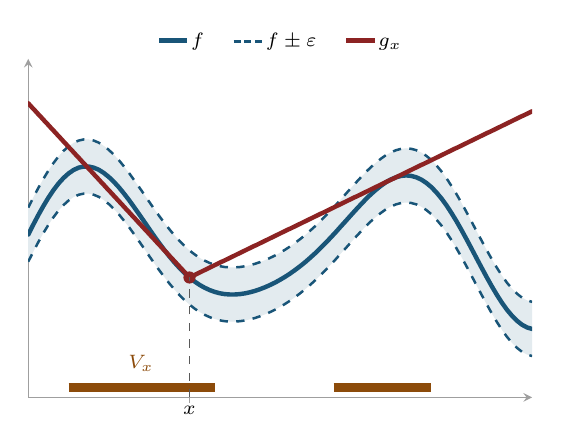
\begin{tikzpicture}
    \begin{axis}[swaxis, width=6.4cm, height=4.3cm, xmin=0, xmax=5, ymin=0.25, ymax=3.0,
        xtick={1.60}, xticklabels={$x$}, title={\scriptsize \textcolor{defcolor}{\rule[0.45ex]{1.3em}{1.6pt}}\,$f$ \quad \textcolor{defcolor}{\rule[0.45ex]{0.32em}{0.9pt}\,\rule[0.45ex]{0.32em}{0.9pt}\,\rule[0.45ex]{0.32em}{0.9pt}}\,$f \pm \varepsilon$ \quad \textcolor{thmcolor}{\rule[0.45ex]{1.3em}{1.6pt}}\,$g_x$}, title style={yshift=-1.2ex, fill=white, fill opacity=0.6, text opacity=1, inner sep=2pt}, ytick=\empty]
      \addplot[draw=none, fill=defcolor!12] coordinates {(0.000,1.792) (0.050,1.873) (0.100,1.951) (0.150,2.024) (0.200,2.092) (0.250,2.153) (0.300,2.207) (0.350,2.252) (0.400,2.289) (0.450,2.317) (0.500,2.336) (0.550,2.345) (0.600,2.345) (0.650,2.336) (0.700,2.319) (0.750,2.293) (0.800,2.260) (0.850,2.221) (0.900,2.176) (0.950,2.126) (1.000,2.073) (1.050,2.016) (1.100,1.958) (1.150,1.899) (1.200,1.839) (1.250,1.780) (1.300,1.723) (1.350,1.668) (1.400,1.616) (1.450,1.567) (1.500,1.522) (1.550,1.481) (1.600,1.444) (1.650,1.412) (1.700,1.384) (1.750,1.361) (1.800,1.342) (1.850,1.327) (1.900,1.316) (1.950,1.309) (2.000,1.306) (2.050,1.306) (2.100,1.309) (2.150,1.315) (2.200,1.324) (2.250,1.335) (2.300,1.349) (2.350,1.365) (2.400,1.383) (2.450,1.403) (2.500,1.426) (2.550,1.450) (2.600,1.477) (2.650,1.506) (2.700,1.537) (2.750,1.570) (2.800,1.606) (2.850,1.643) (2.900,1.683) (2.950,1.724) (3.000,1.767) (3.050,1.811) (3.100,1.857) (3.150,1.902) (3.200,1.948) (3.250,1.993) (3.300,2.037) (3.350,2.080) (3.400,2.120) (3.450,2.156) (3.500,2.189) (3.550,2.218) (3.600,2.241) (3.650,2.258) (3.700,2.269) (3.750,2.273) (3.800,2.269) (3.850,2.258) (3.900,2.239) (3.950,2.212) (4.000,2.178) (4.050,2.135) (4.100,2.086) (4.150,2.030) (4.200,1.967) (4.250,1.900) (4.300,1.828) (4.350,1.753) (4.400,1.676) (4.450,1.598) (4.500,1.521) (4.550,1.445) (4.600,1.372) (4.650,1.303) (4.700,1.239) (4.750,1.182) (4.800,1.133) (4.850,1.092) (4.900,1.060) (4.950,1.038) (5.000,1.026) (5.000,0.586) (4.950,0.598) (4.900,0.620) (4.850,0.652) (4.800,0.693) (4.750,0.742) (4.700,0.799) (4.650,0.863) (4.600,0.932) (4.550,1.005) (4.500,1.081) (4.450,1.158) (4.400,1.236) (4.350,1.313) (4.300,1.388) (4.250,1.460) (4.200,1.527) (4.150,1.590) (4.100,1.646) (4.050,1.695) (4.000,1.738) (3.950,1.772) (3.900,1.799) (3.850,1.818) (3.800,1.829) (3.750,1.833) (3.700,1.829) (3.650,1.818) (3.600,1.801) (3.550,1.778) (3.500,1.749) (3.450,1.716) (3.400,1.680) (3.350,1.640) (3.300,1.597) (3.250,1.553) (3.200,1.508) (3.150,1.462) (3.100,1.417) (3.050,1.371) (3.000,1.327) (2.950,1.284) (2.900,1.243) (2.850,1.203) (2.800,1.166) (2.750,1.130) (2.700,1.097) (2.650,1.066) (2.600,1.037) (2.550,1.010) (2.500,0.986) (2.450,0.963) (2.400,0.943) (2.350,0.925) (2.300,0.909) (2.250,0.895) (2.200,0.884) (2.150,0.875) (2.100,0.869) (2.050,0.866) (2.000,0.866) (1.950,0.869) (1.900,0.876) (1.850,0.887) (1.800,0.902) (1.750,0.921) (1.700,0.944) (1.650,0.972) (1.600,1.004) (1.550,1.041) (1.500,1.082) (1.450,1.127) (1.400,1.176) (1.350,1.228) (1.300,1.283) (1.250,1.340) (1.200,1.399) (1.150,1.459) (1.100,1.518) (1.050,1.576) (1.000,1.633) (0.950,1.686) (0.900,1.736) (0.850,1.781) (0.800,1.820) (0.750,1.853) (0.700,1.879) (0.650,1.896) (0.600,1.905) (0.550,1.905) (0.500,1.896) (0.450,1.877) (0.400,1.849) (0.350,1.812) (0.300,1.767) (0.250,1.713) (0.200,1.652) (0.150,1.584) (0.100,1.511) (0.050,1.433) (0.000,1.352)} -- cycle;
      \addplot[defcolor, dashed, line width=0.9pt] coordinates {(0.000,1.792) (0.050,1.873) (0.100,1.951) (0.150,2.024) (0.200,2.092) (0.250,2.153) (0.300,2.207) (0.350,2.252) (0.400,2.289) (0.450,2.317) (0.500,2.336) (0.550,2.345) (0.600,2.345) (0.650,2.336) (0.700,2.319) (0.750,2.293) (0.800,2.260) (0.850,2.221) (0.900,2.176) (0.950,2.126) (1.000,2.073) (1.050,2.016) (1.100,1.958) (1.150,1.899) (1.200,1.839) (1.250,1.780) (1.300,1.723) (1.350,1.668) (1.400,1.616) (1.450,1.567) (1.500,1.522) (1.550,1.481) (1.600,1.444) (1.650,1.412) (1.700,1.384) (1.750,1.361) (1.800,1.342) (1.850,1.327) (1.900,1.316) (1.950,1.309) (2.000,1.306) (2.050,1.306) (2.100,1.309) (2.150,1.315) (2.200,1.324) (2.250,1.335) (2.300,1.349) (2.350,1.365) (2.400,1.383) (2.450,1.403) (2.500,1.426) (2.550,1.450) (2.600,1.477) (2.650,1.506) (2.700,1.537) (2.750,1.570) (2.800,1.606) (2.850,1.643) (2.900,1.683) (2.950,1.724) (3.000,1.767) (3.050,1.811) (3.100,1.857) (3.150,1.902) (3.200,1.948) (3.250,1.993) (3.300,2.037) (3.350,2.080) (3.400,2.120) (3.450,2.156) (3.500,2.189) (3.550,2.218) (3.600,2.241) (3.650,2.258) (3.700,2.269) (3.750,2.273) (3.800,2.269) (3.850,2.258) (3.900,2.239) (3.950,2.212) (4.000,2.178) (4.050,2.135) (4.100,2.086) (4.150,2.030) (4.200,1.967) (4.250,1.900) (4.300,1.828) (4.350,1.753) (4.400,1.676) (4.450,1.598) (4.500,1.521) (4.550,1.445) (4.600,1.372) (4.650,1.303) (4.700,1.239) (4.750,1.182) (4.800,1.133) (4.850,1.092) (4.900,1.060) (4.950,1.038) (5.000,1.026)};
      \addplot[defcolor, dashed, line width=0.9pt] coordinates {(0.000,1.352) (0.050,1.433) (0.100,1.511) (0.150,1.584) (0.200,1.652) (0.250,1.713) (0.300,1.767) (0.350,1.812) (0.400,1.849) (0.450,1.877) (0.500,1.896) (0.550,1.905) (0.600,1.905) (0.650,1.896) (0.700,1.879) (0.750,1.853) (0.800,1.820) (0.850,1.781) (0.900,1.736) (0.950,1.686) (1.000,1.633) (1.050,1.576) (1.100,1.518) (1.150,1.459) (1.200,1.399) (1.250,1.340) (1.300,1.283) (1.350,1.228) (1.400,1.176) (1.450,1.127) (1.500,1.082) (1.550,1.041) (1.600,1.004) (1.650,0.972) (1.700,0.944) (1.750,0.921) (1.800,0.902) (1.850,0.887) (1.900,0.876) (1.950,0.869) (2.000,0.866) (2.050,0.866) (2.100,0.869) (2.150,0.875) (2.200,0.884) (2.250,0.895) (2.300,0.909) (2.350,0.925) (2.400,0.943) (2.450,0.963) (2.500,0.986) (2.550,1.010) (2.600,1.037) (2.650,1.066) (2.700,1.097) (2.750,1.130) (2.800,1.166) (2.850,1.203) (2.900,1.243) (2.950,1.284) (3.000,1.327) (3.050,1.371) (3.100,1.417) (3.150,1.462) (3.200,1.508) (3.250,1.553) (3.300,1.597) (3.350,1.640) (3.400,1.680) (3.450,1.716) (3.500,1.749) (3.550,1.778) (3.600,1.801) (3.650,1.818) (3.700,1.829) (3.750,1.833) (3.800,1.829) (3.850,1.818) (3.900,1.799) (3.950,1.772) (4.000,1.738) (4.050,1.695) (4.100,1.646) (4.150,1.590) (4.200,1.527) (4.250,1.460) (4.300,1.388) (4.350,1.313) (4.400,1.236) (4.450,1.158) (4.500,1.081) (4.550,1.005) (4.600,0.932) (4.650,0.863) (4.700,0.799) (4.750,0.742) (4.800,0.693) (4.850,0.652) (4.900,0.620) (4.950,0.598) (5.000,0.586)};
      \addplot[defcolor, curveln] coordinates {(0.000,1.572) (0.050,1.653) (0.100,1.731) (0.150,1.804) (0.200,1.872) (0.250,1.933) (0.300,1.987) (0.350,2.032) (0.400,2.069) (0.450,2.097) (0.500,2.116) (0.550,2.125) (0.600,2.125) (0.650,2.116) (0.700,2.099) (0.750,2.073) (0.800,2.040) (0.850,2.001) (0.900,1.956) (0.950,1.906) (1.000,1.853) (1.050,1.796) (1.100,1.738) (1.150,1.679) (1.200,1.619) (1.250,1.560) (1.300,1.503) (1.350,1.448) (1.400,1.396) (1.450,1.347) (1.500,1.302) (1.550,1.261) (1.600,1.224) (1.650,1.192) (1.700,1.164) (1.750,1.141) (1.800,1.122) (1.850,1.107) (1.900,1.096) (1.950,1.089) (2.000,1.086) (2.050,1.086) (2.100,1.089) (2.150,1.095) (2.200,1.104) (2.250,1.115) (2.300,1.129) (2.350,1.145) (2.400,1.163) (2.450,1.183) (2.500,1.206) (2.550,1.230) (2.600,1.257) (2.650,1.286) (2.700,1.317) (2.750,1.350) (2.800,1.386) (2.850,1.423) (2.900,1.463) (2.950,1.504) (3.000,1.547) (3.050,1.591) (3.100,1.637) (3.150,1.682) (3.200,1.728) (3.250,1.773) (3.300,1.817) (3.350,1.860) (3.400,1.900) (3.450,1.936) (3.500,1.969) (3.550,1.998) (3.600,2.021) (3.650,2.038) (3.700,2.049) (3.750,2.053) (3.800,2.049) (3.850,2.038) (3.900,2.019) (3.950,1.992) (4.000,1.958) (4.050,1.915) (4.100,1.866) (4.150,1.810) (4.200,1.747) (4.250,1.680) (4.300,1.608) (4.350,1.533) (4.400,1.456) (4.450,1.378) (4.500,1.301) (4.550,1.225) (4.600,1.152) (4.650,1.083) (4.700,1.019) (4.750,0.962) (4.800,0.913) (4.850,0.872) (4.900,0.840) (4.950,0.818) (5.000,0.806)};
      \addplot[thmcolor, curveln] coordinates {(0.000,2.639) (0.020,2.621) (0.040,2.603) (0.060,2.586) (0.080,2.568) (0.100,2.550) (0.120,2.533) (0.140,2.515) (0.160,2.497) (0.180,2.480) (0.200,2.462) (0.220,2.444) (0.240,2.427) (0.260,2.409) (0.280,2.391) (0.300,2.374) (0.320,2.356) (0.340,2.338) (0.360,2.320) (0.380,2.303) (0.400,2.285) (0.420,2.267) (0.440,2.250) (0.460,2.232) (0.480,2.214) (0.500,2.197) (0.520,2.179) (0.540,2.161) (0.560,2.144) (0.580,2.126) (0.600,2.108) (0.620,2.091) (0.640,2.073) (0.660,2.055) (0.680,2.038) (0.700,2.020) (0.720,2.002) (0.740,1.985) (0.760,1.967) (0.780,1.949) (0.800,1.932) (0.820,1.914) (0.840,1.896) (0.860,1.879) (0.880,1.861) (0.900,1.843) (0.920,1.826) (0.940,1.808) (0.960,1.790) (0.980,1.772) (1.000,1.755) (1.020,1.737) (1.040,1.719) (1.060,1.702) (1.080,1.684) (1.100,1.666) (1.120,1.649) (1.140,1.631) (1.160,1.613) (1.180,1.596) (1.200,1.578) (1.220,1.560) (1.240,1.543) (1.260,1.525) (1.280,1.507) (1.300,1.490) (1.320,1.472) (1.340,1.454) (1.360,1.437) (1.380,1.419) (1.400,1.401) (1.420,1.384) (1.440,1.366) (1.460,1.348) (1.480,1.331) (1.500,1.313) (1.520,1.295) (1.540,1.278) (1.560,1.260) (1.580,1.242) (1.600,1.224) (1.620,1.232) (1.640,1.240) (1.660,1.248) (1.680,1.256) (1.700,1.264) (1.720,1.272) (1.740,1.280) (1.760,1.288) (1.780,1.296) (1.800,1.304) (1.820,1.312) (1.840,1.320) (1.860,1.328) (1.880,1.336) (1.900,1.344) (1.920,1.352) (1.940,1.359) (1.960,1.367) (1.980,1.375) (2.000,1.383) (2.020,1.391) (2.040,1.399) (2.060,1.407) (2.080,1.415) (2.100,1.423) (2.120,1.431) (2.140,1.439) (2.160,1.447) (2.180,1.455) (2.200,1.463) (2.220,1.471) (2.240,1.479) (2.260,1.486) (2.280,1.494) (2.300,1.502) (2.320,1.510) (2.340,1.518) (2.360,1.526) (2.380,1.534) (2.400,1.542) (2.420,1.550) (2.440,1.558) (2.460,1.566) (2.480,1.574) (2.500,1.582) (2.520,1.590) (2.540,1.598) (2.560,1.606) (2.580,1.614) (2.600,1.621) (2.620,1.629) (2.640,1.637) (2.660,1.645) (2.680,1.653) (2.700,1.661) (2.720,1.669) (2.740,1.677) (2.760,1.685) (2.780,1.693) (2.800,1.701) (2.820,1.709) (2.840,1.717) (2.860,1.725) (2.880,1.733) (2.900,1.741) (2.920,1.748) (2.940,1.756) (2.960,1.764) (2.980,1.772) (3.000,1.780) (3.020,1.788) (3.040,1.796) (3.060,1.804) (3.080,1.812) (3.100,1.820) (3.120,1.828) (3.140,1.836) (3.160,1.844) (3.180,1.852) (3.200,1.860) (3.220,1.868) (3.240,1.876) (3.260,1.883) (3.280,1.891) (3.300,1.899) (3.320,1.907) (3.340,1.915) (3.360,1.923) (3.380,1.931) (3.400,1.939) (3.420,1.947) (3.440,1.955) (3.460,1.963) (3.480,1.971) (3.500,1.979) (3.520,1.987) (3.540,1.995) (3.560,2.003) (3.580,2.011) (3.600,2.018) (3.620,2.026) (3.640,2.034) (3.660,2.042) (3.680,2.050) (3.700,2.058) (3.720,2.066) (3.740,2.074) (3.760,2.082) (3.780,2.090) (3.800,2.098) (3.820,2.106) (3.840,2.114) (3.860,2.122) (3.880,2.130) (3.900,2.138) (3.920,2.145) (3.940,2.153) (3.960,2.161) (3.980,2.169) (4.000,2.177) (4.020,2.185) (4.040,2.193) (4.060,2.201) (4.080,2.209) (4.100,2.217) (4.120,2.225) (4.140,2.233) (4.160,2.241) (4.180,2.249) (4.200,2.257) (4.220,2.265) (4.240,2.273) (4.260,2.280) (4.280,2.288) (4.300,2.296) (4.320,2.304) (4.340,2.312) (4.360,2.320) (4.380,2.328) (4.400,2.336) (4.420,2.344) (4.440,2.352) (4.460,2.360) (4.480,2.368) (4.500,2.376) (4.520,2.384) (4.540,2.392) (4.560,2.400) (4.580,2.407) (4.600,2.415) (4.620,2.423) (4.640,2.431) (4.660,2.439) (4.680,2.447) (4.700,2.455) (4.720,2.463) (4.740,2.471) (4.760,2.479) (4.780,2.487) (4.800,2.495) (4.820,2.503) (4.840,2.511) (4.860,2.519) (4.880,2.527) (4.900,2.535) (4.920,2.542) (4.940,2.550) (4.960,2.558) (4.980,2.566) (5.000,2.574)};
      \draw[excolor, line width=3pt] (axis cs:0.400,0.33) -- (axis cs:1.850,0.33);
      \draw[excolor, line width=3pt] (axis cs:3.030,0.33) -- (axis cs:4.000,0.33);
      \node[excolor, font=\scriptsize, anchor=south] at (axis cs:1.12,0.38) {$V_x$};
      \fill[thmcolor] (axis cs:1.60,1.224) circle (2.2pt);
      \draw[gray!70!black, dashed] (axis cs:1.60,0.25) -- (axis cs:1.60,1.224);
    \end{axis}
  \end{tikzpicture}
    \end{column}
  \end{columns}

  \note{
    For each point "x" of capital "K", take the function "g" sub "x" from
    Step 3. At the point "x" it equals "f", so it is strictly below "f" plus
    epsilon there. By continuity, the same holds on an open set containing
    "x", called capital "V" sub "x". This is equation 59. In the picture,
    the red curve is one such "g" sub "x". It lies above the lower dashed
    curve everywhere, but it stays below the upper dashed curve only near
    "x". The thick amber segments on the axis mark where the red curve is
    inside the shaded tube. The segment containing "x" can serve as capital
    "V" sub "x".
  }
\end{frame}

% --- Build 2/3 ---
\begin{frame}{Proof of Theorem 7.32 --- Step 4}
  \begin{columns}[T]
    \begin{column}{0.5\textwidth}
      \small
      \begin{proofblock}{Proof of Step 4}
        For each $x \in K$ take $g_x$ from Step 3. By continuity of $g_x$ there
        are open sets $V_x \ni x$ with
        \[
          g_x(t) < f(t) + \varepsilon \quad (t \in V_x). \tag{59}
        \]
        $K$ is compact: there are $x_1, \dots, x_m$ with
        \[
          K \subset V_{x_1} \cup \cdots \cup V_{x_m}. \tag{60}
        \]
        Put $h = \min(g_{x_1}, \dots, g_{x_m})$. By Step 2, $h \in \mathscr{B}$.
      \end{proofblock}
    \end{column}
    \begin{column}{0.48\textwidth}
      \centering
  \vspace{0.6em}
  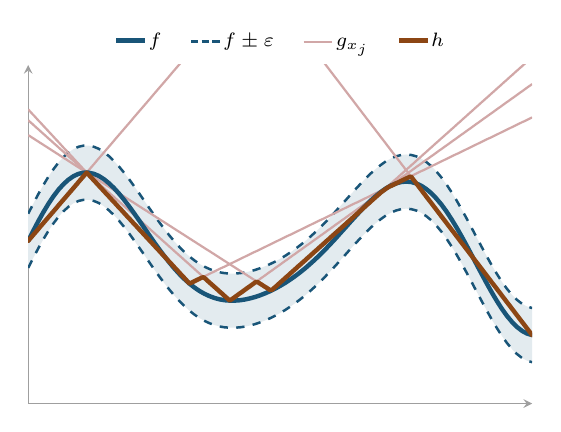
\begin{tikzpicture}
    \begin{axis}[swaxis, width=6.4cm, height=4.3cm, xmin=0, xmax=5, ymin=0.25, ymax=3.0,
        xtick=\empty, title={\scriptsize \textcolor{defcolor}{\rule[0.45ex]{1.3em}{1.6pt}}\,$f$ \quad \textcolor{defcolor}{\rule[0.45ex]{0.32em}{0.9pt}\,\rule[0.45ex]{0.32em}{0.9pt}\,\rule[0.45ex]{0.32em}{0.9pt}}\,$f \pm \varepsilon$ \quad \textcolor{thmcolor!40}{\rule[0.45ex]{1.3em}{0.8pt}}\,$g_{x_j}$ \quad \textcolor{mAccent}{\rule[0.45ex]{1.3em}{1.6pt}}\,$h$}, title style={yshift=-1.2ex, fill=white, fill opacity=0.6, text opacity=1, inner sep=2pt}, ytick=\empty]
      \addplot[draw=none, fill=defcolor!12] coordinates {(0.000,1.792) (0.050,1.873) (0.100,1.951) (0.150,2.024) (0.200,2.092) (0.250,2.153) (0.300,2.207) (0.350,2.252) (0.400,2.289) (0.450,2.317) (0.500,2.336) (0.550,2.345) (0.600,2.345) (0.650,2.336) (0.700,2.319) (0.750,2.293) (0.800,2.260) (0.850,2.221) (0.900,2.176) (0.950,2.126) (1.000,2.073) (1.050,2.016) (1.100,1.958) (1.150,1.899) (1.200,1.839) (1.250,1.780) (1.300,1.723) (1.350,1.668) (1.400,1.616) (1.450,1.567) (1.500,1.522) (1.550,1.481) (1.600,1.444) (1.650,1.412) (1.700,1.384) (1.750,1.361) (1.800,1.342) (1.850,1.327) (1.900,1.316) (1.950,1.309) (2.000,1.306) (2.050,1.306) (2.100,1.309) (2.150,1.315) (2.200,1.324) (2.250,1.335) (2.300,1.349) (2.350,1.365) (2.400,1.383) (2.450,1.403) (2.500,1.426) (2.550,1.450) (2.600,1.477) (2.650,1.506) (2.700,1.537) (2.750,1.570) (2.800,1.606) (2.850,1.643) (2.900,1.683) (2.950,1.724) (3.000,1.767) (3.050,1.811) (3.100,1.857) (3.150,1.902) (3.200,1.948) (3.250,1.993) (3.300,2.037) (3.350,2.080) (3.400,2.120) (3.450,2.156) (3.500,2.189) (3.550,2.218) (3.600,2.241) (3.650,2.258) (3.700,2.269) (3.750,2.273) (3.800,2.269) (3.850,2.258) (3.900,2.239) (3.950,2.212) (4.000,2.178) (4.050,2.135) (4.100,2.086) (4.150,2.030) (4.200,1.967) (4.250,1.900) (4.300,1.828) (4.350,1.753) (4.400,1.676) (4.450,1.598) (4.500,1.521) (4.550,1.445) (4.600,1.372) (4.650,1.303) (4.700,1.239) (4.750,1.182) (4.800,1.133) (4.850,1.092) (4.900,1.060) (4.950,1.038) (5.000,1.026) (5.000,0.586) (4.950,0.598) (4.900,0.620) (4.850,0.652) (4.800,0.693) (4.750,0.742) (4.700,0.799) (4.650,0.863) (4.600,0.932) (4.550,1.005) (4.500,1.081) (4.450,1.158) (4.400,1.236) (4.350,1.313) (4.300,1.388) (4.250,1.460) (4.200,1.527) (4.150,1.590) (4.100,1.646) (4.050,1.695) (4.000,1.738) (3.950,1.772) (3.900,1.799) (3.850,1.818) (3.800,1.829) (3.750,1.833) (3.700,1.829) (3.650,1.818) (3.600,1.801) (3.550,1.778) (3.500,1.749) (3.450,1.716) (3.400,1.680) (3.350,1.640) (3.300,1.597) (3.250,1.553) (3.200,1.508) (3.150,1.462) (3.100,1.417) (3.050,1.371) (3.000,1.327) (2.950,1.284) (2.900,1.243) (2.850,1.203) (2.800,1.166) (2.750,1.130) (2.700,1.097) (2.650,1.066) (2.600,1.037) (2.550,1.010) (2.500,0.986) (2.450,0.963) (2.400,0.943) (2.350,0.925) (2.300,0.909) (2.250,0.895) (2.200,0.884) (2.150,0.875) (2.100,0.869) (2.050,0.866) (2.000,0.866) (1.950,0.869) (1.900,0.876) (1.850,0.887) (1.800,0.902) (1.750,0.921) (1.700,0.944) (1.650,0.972) (1.600,1.004) (1.550,1.041) (1.500,1.082) (1.450,1.127) (1.400,1.176) (1.350,1.228) (1.300,1.283) (1.250,1.340) (1.200,1.399) (1.150,1.459) (1.100,1.518) (1.050,1.576) (1.000,1.633) (0.950,1.686) (0.900,1.736) (0.850,1.781) (0.800,1.820) (0.750,1.853) (0.700,1.879) (0.650,1.896) (0.600,1.905) (0.550,1.905) (0.500,1.896) (0.450,1.877) (0.400,1.849) (0.350,1.812) (0.300,1.767) (0.250,1.713) (0.200,1.652) (0.150,1.584) (0.100,1.511) (0.050,1.433) (0.000,1.352)} -- cycle;
      \addplot[defcolor, dashed, line width=0.9pt] coordinates {(0.000,1.792) (0.050,1.873) (0.100,1.951) (0.150,2.024) (0.200,2.092) (0.250,2.153) (0.300,2.207) (0.350,2.252) (0.400,2.289) (0.450,2.317) (0.500,2.336) (0.550,2.345) (0.600,2.345) (0.650,2.336) (0.700,2.319) (0.750,2.293) (0.800,2.260) (0.850,2.221) (0.900,2.176) (0.950,2.126) (1.000,2.073) (1.050,2.016) (1.100,1.958) (1.150,1.899) (1.200,1.839) (1.250,1.780) (1.300,1.723) (1.350,1.668) (1.400,1.616) (1.450,1.567) (1.500,1.522) (1.550,1.481) (1.600,1.444) (1.650,1.412) (1.700,1.384) (1.750,1.361) (1.800,1.342) (1.850,1.327) (1.900,1.316) (1.950,1.309) (2.000,1.306) (2.050,1.306) (2.100,1.309) (2.150,1.315) (2.200,1.324) (2.250,1.335) (2.300,1.349) (2.350,1.365) (2.400,1.383) (2.450,1.403) (2.500,1.426) (2.550,1.450) (2.600,1.477) (2.650,1.506) (2.700,1.537) (2.750,1.570) (2.800,1.606) (2.850,1.643) (2.900,1.683) (2.950,1.724) (3.000,1.767) (3.050,1.811) (3.100,1.857) (3.150,1.902) (3.200,1.948) (3.250,1.993) (3.300,2.037) (3.350,2.080) (3.400,2.120) (3.450,2.156) (3.500,2.189) (3.550,2.218) (3.600,2.241) (3.650,2.258) (3.700,2.269) (3.750,2.273) (3.800,2.269) (3.850,2.258) (3.900,2.239) (3.950,2.212) (4.000,2.178) (4.050,2.135) (4.100,2.086) (4.150,2.030) (4.200,1.967) (4.250,1.900) (4.300,1.828) (4.350,1.753) (4.400,1.676) (4.450,1.598) (4.500,1.521) (4.550,1.445) (4.600,1.372) (4.650,1.303) (4.700,1.239) (4.750,1.182) (4.800,1.133) (4.850,1.092) (4.900,1.060) (4.950,1.038) (5.000,1.026)};
      \addplot[defcolor, dashed, line width=0.9pt] coordinates {(0.000,1.352) (0.050,1.433) (0.100,1.511) (0.150,1.584) (0.200,1.652) (0.250,1.713) (0.300,1.767) (0.350,1.812) (0.400,1.849) (0.450,1.877) (0.500,1.896) (0.550,1.905) (0.600,1.905) (0.650,1.896) (0.700,1.879) (0.750,1.853) (0.800,1.820) (0.850,1.781) (0.900,1.736) (0.950,1.686) (1.000,1.633) (1.050,1.576) (1.100,1.518) (1.150,1.459) (1.200,1.399) (1.250,1.340) (1.300,1.283) (1.350,1.228) (1.400,1.176) (1.450,1.127) (1.500,1.082) (1.550,1.041) (1.600,1.004) (1.650,0.972) (1.700,0.944) (1.750,0.921) (1.800,0.902) (1.850,0.887) (1.900,0.876) (1.950,0.869) (2.000,0.866) (2.050,0.866) (2.100,0.869) (2.150,0.875) (2.200,0.884) (2.250,0.895) (2.300,0.909) (2.350,0.925) (2.400,0.943) (2.450,0.963) (2.500,0.986) (2.550,1.010) (2.600,1.037) (2.650,1.066) (2.700,1.097) (2.750,1.130) (2.800,1.166) (2.850,1.203) (2.900,1.243) (2.950,1.284) (3.000,1.327) (3.050,1.371) (3.100,1.417) (3.150,1.462) (3.200,1.508) (3.250,1.553) (3.300,1.597) (3.350,1.640) (3.400,1.680) (3.450,1.716) (3.500,1.749) (3.550,1.778) (3.600,1.801) (3.650,1.818) (3.700,1.829) (3.750,1.833) (3.800,1.829) (3.850,1.818) (3.900,1.799) (3.950,1.772) (4.000,1.738) (4.050,1.695) (4.100,1.646) (4.150,1.590) (4.200,1.527) (4.250,1.460) (4.300,1.388) (4.350,1.313) (4.400,1.236) (4.450,1.158) (4.500,1.081) (4.550,1.005) (4.600,0.932) (4.650,0.863) (4.700,0.799) (4.750,0.742) (4.800,0.693) (4.850,0.652) (4.900,0.620) (4.950,0.598) (5.000,0.586)};
      \addplot[thmcolor!40, line width=0.8pt] coordinates {(0.000,2.639) (0.020,2.621) (0.040,2.603) (0.060,2.586) (0.080,2.568) (0.100,2.550) (0.120,2.533) (0.140,2.515) (0.160,2.497) (0.180,2.480) (0.200,2.462) (0.220,2.444) (0.240,2.427) (0.260,2.409) (0.280,2.391) (0.300,2.374) (0.320,2.356) (0.340,2.338) (0.360,2.320) (0.380,2.303) (0.400,2.285) (0.420,2.267) (0.440,2.250) (0.460,2.232) (0.480,2.214) (0.500,2.197) (0.520,2.179) (0.540,2.161) (0.560,2.144) (0.580,2.126) (0.600,2.108) (0.620,2.091) (0.640,2.073) (0.660,2.055) (0.680,2.038) (0.700,2.020) (0.720,2.002) (0.740,1.985) (0.760,1.967) (0.780,1.949) (0.800,1.932) (0.820,1.914) (0.840,1.896) (0.860,1.879) (0.880,1.861) (0.900,1.843) (0.920,1.826) (0.940,1.808) (0.960,1.790) (0.980,1.772) (1.000,1.755) (1.020,1.737) (1.040,1.719) (1.060,1.702) (1.080,1.684) (1.100,1.666) (1.120,1.649) (1.140,1.631) (1.160,1.613) (1.180,1.596) (1.200,1.578) (1.220,1.560) (1.240,1.543) (1.260,1.525) (1.280,1.507) (1.300,1.490) (1.320,1.472) (1.340,1.454) (1.360,1.437) (1.380,1.419) (1.400,1.401) (1.420,1.384) (1.440,1.366) (1.460,1.348) (1.480,1.331) (1.500,1.313) (1.520,1.295) (1.540,1.278) (1.560,1.260) (1.580,1.242) (1.600,1.224) (1.620,1.232) (1.640,1.240) (1.660,1.248) (1.680,1.256) (1.700,1.264) (1.720,1.272) (1.740,1.280) (1.760,1.288) (1.780,1.296) (1.800,1.304) (1.820,1.312) (1.840,1.320) (1.860,1.328) (1.880,1.336) (1.900,1.344) (1.920,1.352) (1.940,1.359) (1.960,1.367) (1.980,1.375) (2.000,1.383) (2.020,1.391) (2.040,1.399) (2.060,1.407) (2.080,1.415) (2.100,1.423) (2.120,1.431) (2.140,1.439) (2.160,1.447) (2.180,1.455) (2.200,1.463) (2.220,1.471) (2.240,1.479) (2.260,1.486) (2.280,1.494) (2.300,1.502) (2.320,1.510) (2.340,1.518) (2.360,1.526) (2.380,1.534) (2.400,1.542) (2.420,1.550) (2.440,1.558) (2.460,1.566) (2.480,1.574) (2.500,1.582) (2.520,1.590) (2.540,1.598) (2.560,1.606) (2.580,1.614) (2.600,1.621) (2.620,1.629) (2.640,1.637) (2.660,1.645) (2.680,1.653) (2.700,1.661) (2.720,1.669) (2.740,1.677) (2.760,1.685) (2.780,1.693) (2.800,1.701) (2.820,1.709) (2.840,1.717) (2.860,1.725) (2.880,1.733) (2.900,1.741) (2.920,1.748) (2.940,1.756) (2.960,1.764) (2.980,1.772) (3.000,1.780) (3.020,1.788) (3.040,1.796) (3.060,1.804) (3.080,1.812) (3.100,1.820) (3.120,1.828) (3.140,1.836) (3.160,1.844) (3.180,1.852) (3.200,1.860) (3.220,1.868) (3.240,1.876) (3.260,1.883) (3.280,1.891) (3.300,1.899) (3.320,1.907) (3.340,1.915) (3.360,1.923) (3.380,1.931) (3.400,1.939) (3.420,1.947) (3.440,1.955) (3.460,1.963) (3.480,1.971) (3.500,1.979) (3.520,1.987) (3.540,1.995) (3.560,2.003) (3.580,2.011) (3.600,2.018) (3.620,2.026) (3.640,2.034) (3.660,2.042) (3.680,2.050) (3.700,2.058) (3.720,2.066) (3.740,2.074) (3.760,2.082) (3.780,2.090) (3.800,2.098) (3.820,2.106) (3.840,2.114) (3.860,2.122) (3.880,2.130) (3.900,2.138) (3.920,2.145) (3.940,2.153) (3.960,2.161) (3.980,2.169) (4.000,2.177) (4.020,2.185) (4.040,2.193) (4.060,2.201) (4.080,2.209) (4.100,2.217) (4.120,2.225) (4.140,2.233) (4.160,2.241) (4.180,2.249) (4.200,2.257) (4.220,2.265) (4.240,2.273) (4.260,2.280) (4.280,2.288) (4.300,2.296) (4.320,2.304) (4.340,2.312) (4.360,2.320) (4.380,2.328) (4.400,2.336) (4.420,2.344) (4.440,2.352) (4.460,2.360) (4.480,2.368) (4.500,2.376) (4.520,2.384) (4.540,2.392) (4.560,2.400) (4.580,2.407) (4.600,2.415) (4.620,2.423) (4.640,2.431) (4.660,2.439) (4.680,2.447) (4.700,2.455) (4.720,2.463) (4.740,2.471) (4.760,2.479) (4.780,2.487) (4.800,2.495) (4.820,2.503) (4.840,2.511) (4.860,2.519) (4.880,2.527) (4.900,2.535) (4.920,2.542) (4.940,2.550) (4.960,2.558) (4.980,2.566) (5.000,2.574)};
      \addplot[thmcolor!40, line width=0.8pt] coordinates {(0.000,6.165) (0.020,6.143) (0.040,6.122) (0.060,6.100) (0.080,6.079) (0.100,6.057) (0.120,6.036) (0.140,6.015) (0.160,5.993) (0.180,5.972) (0.200,5.950) (0.220,5.929) (0.240,5.907) (0.260,5.886) (0.280,5.864) (0.300,5.843) (0.320,5.822) (0.340,5.800) (0.360,5.779) (0.380,5.757) (0.400,5.736) (0.420,5.714) (0.440,5.693) (0.460,5.672) (0.480,5.650) (0.500,5.629) (0.520,5.607) (0.540,5.586) (0.560,5.564) (0.580,5.543) (0.600,5.522) (0.620,5.500) (0.640,5.479) (0.660,5.457) (0.680,5.436) (0.700,5.414) (0.720,5.393) (0.740,5.371) (0.760,5.350) (0.780,5.329) (0.800,5.307) (0.820,5.286) (0.840,5.264) (0.860,5.243) (0.880,5.221) (0.900,5.200) (0.920,5.179) (0.940,5.157) (0.960,5.136) (0.980,5.114) (1.000,5.093) (1.020,5.071) (1.040,5.050) (1.060,5.029) (1.080,5.007) (1.100,4.986) (1.120,4.964) (1.140,4.943) (1.160,4.921) (1.180,4.900) (1.200,4.878) (1.220,4.857) (1.240,4.836) (1.260,4.814) (1.280,4.793) (1.300,4.771) (1.320,4.750) (1.340,4.728) (1.360,4.707) (1.380,4.686) (1.400,4.664) (1.420,4.643) (1.440,4.621) (1.460,4.600) (1.480,4.578) (1.500,4.557) (1.520,4.536) (1.540,4.514) (1.560,4.493) (1.580,4.471) (1.600,4.450) (1.620,4.428) (1.640,4.407) (1.660,4.385) (1.680,4.364) (1.700,4.343) (1.720,4.321) (1.740,4.300) (1.760,4.278) (1.780,4.257) (1.800,4.235) (1.820,4.214) (1.840,4.193) (1.860,4.171) (1.880,4.150) (1.900,4.128) (1.920,4.107) (1.940,4.085) (1.960,4.064) (1.980,4.043) (2.000,4.021) (2.020,4.000) (2.040,3.978) (2.060,3.957) (2.080,3.935) (2.100,3.914) (2.120,3.892) (2.140,3.871) (2.160,3.850) (2.180,3.828) (2.200,3.807) (2.220,3.785) (2.240,3.764) (2.260,3.742) (2.280,3.721) (2.300,3.700) (2.320,3.678) (2.340,3.657) (2.360,3.635) (2.380,3.614) (2.400,3.592) (2.420,3.571) (2.440,3.549) (2.460,3.528) (2.480,3.507) (2.500,3.485) (2.520,3.464) (2.540,3.442) (2.560,3.421) (2.580,3.399) (2.600,3.378) (2.620,3.357) (2.640,3.335) (2.660,3.314) (2.680,3.292) (2.700,3.271) (2.720,3.249) (2.740,3.228) (2.760,3.207) (2.780,3.185) (2.800,3.164) (2.820,3.142) (2.840,3.121) (2.860,3.099) (2.880,3.078) (2.900,3.056) (2.920,3.035) (2.940,3.014) (2.960,2.992) (2.980,2.971) (3.000,2.949) (3.020,2.928) (3.040,2.906) (3.060,2.885) (3.080,2.864) (3.100,2.842) (3.120,2.821) (3.140,2.799) (3.160,2.778) (3.180,2.756) (3.200,2.735) (3.220,2.714) (3.240,2.692) (3.260,2.671) (3.280,2.649) (3.300,2.628) (3.320,2.606) (3.340,2.585) (3.360,2.563) (3.380,2.542) (3.400,2.521) (3.420,2.499) (3.440,2.478) (3.460,2.456) (3.480,2.435) (3.500,2.413) (3.520,2.392) (3.540,2.371) (3.560,2.349) (3.580,2.328) (3.600,2.306) (3.620,2.285) (3.640,2.263) (3.660,2.242) (3.680,2.221) (3.700,2.199) (3.720,2.178) (3.740,2.156) (3.760,2.135) (3.780,2.113) (3.800,2.092) (3.820,2.070) (3.840,2.049) (3.860,2.028) (3.880,2.006) (3.900,1.985) (3.920,1.963) (3.940,1.942) (3.960,1.920) (3.980,1.899) (4.000,1.878) (4.020,1.856) (4.040,1.835) (4.060,1.813) (4.080,1.792) (4.100,1.770) (4.120,1.749) (4.140,1.728) (4.160,1.706) (4.180,1.685) (4.200,1.663) (4.220,1.642) (4.240,1.620) (4.260,1.599) (4.280,1.577) (4.300,1.556) (4.320,1.535) (4.340,1.513) (4.360,1.492) (4.380,1.470) (4.400,1.449) (4.420,1.427) (4.440,1.406) (4.460,1.385) (4.480,1.363) (4.500,1.342) (4.520,1.320) (4.540,1.299) (4.560,1.277) (4.580,1.256) (4.600,1.234) (4.620,1.213) (4.640,1.192) (4.660,1.170) (4.680,1.149) (4.700,1.127) (4.720,1.106) (4.740,1.084) (4.760,1.063) (4.780,1.042) (4.800,1.020) (4.820,0.999) (4.840,0.977) (4.860,0.956) (4.880,0.934) (4.900,0.913) (4.920,0.892) (4.940,0.870) (4.960,0.849) (4.980,0.827) (5.000,0.806)};
      \addplot[thmcolor!40, line width=0.8pt] coordinates {(0.000,1.572) (0.020,1.591) (0.040,1.610) (0.060,1.629) (0.080,1.648) (0.100,1.667) (0.120,1.687) (0.140,1.706) (0.160,1.725) (0.180,1.744) (0.200,1.763) (0.220,1.782) (0.240,1.801) (0.260,1.820) (0.280,1.839) (0.300,1.859) (0.320,1.878) (0.340,1.897) (0.360,1.916) (0.380,1.935) (0.400,1.954) (0.420,1.973) (0.440,1.992) (0.460,2.011) (0.480,2.030) (0.500,2.050) (0.520,2.069) (0.540,2.088) (0.560,2.107) (0.580,2.126) (0.600,2.145) (0.620,2.164) (0.640,2.183) (0.660,2.202) (0.680,2.222) (0.700,2.241) (0.720,2.260) (0.740,2.279) (0.760,2.298) (0.780,2.317) (0.800,2.336) (0.820,2.355) (0.840,2.374) (0.860,2.394) (0.880,2.413) (0.900,2.432) (0.920,2.451) (0.940,2.470) (0.960,2.489) (0.980,2.508) (1.000,2.527) (1.020,2.546) (1.040,2.566) (1.060,2.585) (1.080,2.604) (1.100,2.623) (1.120,2.642) (1.140,2.661) (1.160,2.680) (1.180,2.699) (1.200,2.718) (1.220,2.737) (1.240,2.757) (1.260,2.776) (1.280,2.795) (1.300,2.814) (1.320,2.833) (1.340,2.852) (1.360,2.871) (1.380,2.890) (1.400,2.909) (1.420,2.929) (1.440,2.948) (1.460,2.967) (1.480,2.986) (1.500,3.005) (1.520,3.024) (1.540,3.043) (1.560,3.062) (1.580,3.081) (1.600,3.101) (1.620,3.120) (1.640,3.139) (1.660,3.158) (1.680,3.177) (1.700,3.196) (1.720,3.215) (1.740,3.234) (1.760,3.253) (1.780,3.272) (1.800,3.292) (1.820,3.311) (1.840,3.330) (1.860,3.349) (1.880,3.368) (1.900,3.387) (1.920,3.406) (1.940,3.425) (1.960,3.444) (1.980,3.464) (2.000,3.483) (2.020,3.502) (2.040,3.521) (2.060,3.540) (2.080,3.559) (2.100,3.578) (2.120,3.597) (2.140,3.616) (2.160,3.636) (2.180,3.655) (2.200,3.674) (2.220,3.693) (2.240,3.712) (2.260,3.731) (2.280,3.750) (2.300,3.769) (2.320,3.788) (2.340,3.808) (2.360,3.827) (2.380,3.846) (2.400,3.865) (2.420,3.884) (2.440,3.903) (2.460,3.922) (2.480,3.941) (2.500,3.960) (2.520,3.979) (2.540,3.999) (2.560,4.018) (2.580,4.037) (2.600,4.056) (2.620,4.075) (2.640,4.094) (2.660,4.113) (2.680,4.132) (2.700,4.151) (2.720,4.171) (2.740,4.190) (2.760,4.209) (2.780,4.228) (2.800,4.247) (2.820,4.266) (2.840,4.285) (2.860,4.304) (2.880,4.323) (2.900,4.343) (2.920,4.362) (2.940,4.381) (2.960,4.400) (2.980,4.419) (3.000,4.438) (3.020,4.457) (3.040,4.476) (3.060,4.495) (3.080,4.514) (3.100,4.534) (3.120,4.553) (3.140,4.572) (3.160,4.591) (3.180,4.610) (3.200,4.629) (3.220,4.648) (3.240,4.667) (3.260,4.686) (3.280,4.706) (3.300,4.725) (3.320,4.744) (3.340,4.763) (3.360,4.782) (3.380,4.801) (3.400,4.820) (3.420,4.839) (3.440,4.858) (3.460,4.878) (3.480,4.897) (3.500,4.916) (3.520,4.935) (3.540,4.954) (3.560,4.973) (3.580,4.992) (3.600,5.011) (3.620,5.030) (3.640,5.050) (3.660,5.069) (3.680,5.088) (3.700,5.107) (3.720,5.126) (3.740,5.145) (3.760,5.164) (3.780,5.183) (3.800,5.202) (3.820,5.221) (3.840,5.241) (3.860,5.260) (3.880,5.279) (3.900,5.298) (3.920,5.317) (3.940,5.336) (3.960,5.355) (3.980,5.374) (4.000,5.393) (4.020,5.413) (4.040,5.432) (4.060,5.451) (4.080,5.470) (4.100,5.489) (4.120,5.508) (4.140,5.527) (4.160,5.546) (4.180,5.565) (4.200,5.585) (4.220,5.604) (4.240,5.623) (4.260,5.642) (4.280,5.661) (4.300,5.680) (4.320,5.699) (4.340,5.718) (4.360,5.737) (4.380,5.756) (4.400,5.776) (4.420,5.795) (4.440,5.814) (4.460,5.833) (4.480,5.852) (4.500,5.871) (4.520,5.890) (4.540,5.909) (4.560,5.928) (4.580,5.948) (4.600,5.967) (4.620,5.986) (4.640,6.005) (4.660,6.024) (4.680,6.043) (4.700,6.062) (4.720,6.081) (4.740,6.100) (4.760,6.120) (4.780,6.139) (4.800,6.158) (4.820,6.177) (4.840,6.196) (4.860,6.215) (4.880,6.234) (4.900,6.253) (4.920,6.272) (4.940,6.291) (4.960,6.311) (4.980,6.330) (5.000,6.349)};
      \addplot[thmcolor!40, line width=0.8pt] coordinates {(0.000,2.430) (0.020,2.420) (0.040,2.409) (0.060,2.399) (0.080,2.388) (0.100,2.378) (0.120,2.367) (0.140,2.357) (0.160,2.346) (0.180,2.336) (0.200,2.325) (0.220,2.315) (0.240,2.304) (0.260,2.294) (0.280,2.283) (0.300,2.273) (0.320,2.262) (0.340,2.252) (0.360,2.241) (0.380,2.231) (0.400,2.220) (0.420,2.210) (0.440,2.199) (0.460,2.189) (0.480,2.178) (0.500,2.168) (0.520,2.157) (0.540,2.147) (0.560,2.137) (0.580,2.126) (0.600,2.116) (0.620,2.105) (0.640,2.095) (0.660,2.084) (0.680,2.074) (0.700,2.063) (0.720,2.053) (0.740,2.042) (0.760,2.032) (0.780,2.021) (0.800,2.011) (0.820,2.000) (0.840,1.990) (0.860,1.979) (0.880,1.969) (0.900,1.958) (0.920,1.948) (0.940,1.937) (0.960,1.927) (0.980,1.916) (1.000,1.906) (1.020,1.895) (1.040,1.885) (1.060,1.874) (1.080,1.864) (1.100,1.853) (1.120,1.843) (1.140,1.832) (1.160,1.822) (1.180,1.812) (1.200,1.801) (1.220,1.791) (1.240,1.780) (1.260,1.770) (1.280,1.759) (1.300,1.749) (1.320,1.738) (1.340,1.728) (1.360,1.717) (1.380,1.707) (1.400,1.696) (1.420,1.686) (1.440,1.675) (1.460,1.665) (1.480,1.654) (1.500,1.644) (1.520,1.633) (1.540,1.623) (1.560,1.612) (1.580,1.602) (1.600,1.591) (1.620,1.581) (1.640,1.570) (1.660,1.560) (1.680,1.549) (1.700,1.539) (1.720,1.528) (1.740,1.518) (1.760,1.507) (1.780,1.497) (1.800,1.487) (1.820,1.476) (1.840,1.466) (1.860,1.455) (1.880,1.445) (1.900,1.434) (1.920,1.424) (1.940,1.413) (1.960,1.403) (1.980,1.392) (2.000,1.382) (2.020,1.371) (2.040,1.361) (2.060,1.350) (2.080,1.340) (2.100,1.329) (2.120,1.319) (2.140,1.308) (2.160,1.298) (2.180,1.287) (2.200,1.277) (2.220,1.266) (2.240,1.256) (2.260,1.245) (2.280,1.235) (2.300,1.224) (2.320,1.214) (2.340,1.203) (2.360,1.193) (2.380,1.182) (2.400,1.172) (2.420,1.174) (2.440,1.189) (2.460,1.203) (2.480,1.218) (2.500,1.233) (2.520,1.247) (2.540,1.262) (2.560,1.277) (2.580,1.291) (2.600,1.306) (2.620,1.321) (2.640,1.335) (2.660,1.350) (2.680,1.365) (2.700,1.379) (2.720,1.394) (2.740,1.408) (2.760,1.423) (2.780,1.438) (2.800,1.452) (2.820,1.467) (2.840,1.482) (2.860,1.496) (2.880,1.511) (2.900,1.526) (2.920,1.540) (2.940,1.555) (2.960,1.570) (2.980,1.584) (3.000,1.599) (3.020,1.614) (3.040,1.628) (3.060,1.643) (3.080,1.657) (3.100,1.672) (3.120,1.687) (3.140,1.701) (3.160,1.716) (3.180,1.731) (3.200,1.745) (3.220,1.760) (3.240,1.775) (3.260,1.789) (3.280,1.804) (3.300,1.819) (3.320,1.833) (3.340,1.848) (3.360,1.863) (3.380,1.877) (3.400,1.892) (3.420,1.907) (3.440,1.921) (3.460,1.936) (3.480,1.950) (3.500,1.965) (3.520,1.980) (3.540,1.994) (3.560,2.009) (3.580,2.024) (3.600,2.038) (3.620,2.053) (3.640,2.068) (3.660,2.082) (3.680,2.097) (3.700,2.112) (3.720,2.126) (3.740,2.141) (3.760,2.156) (3.780,2.170) (3.800,2.185) (3.820,2.199) (3.840,2.214) (3.860,2.229) (3.880,2.243) (3.900,2.258) (3.920,2.273) (3.940,2.287) (3.960,2.302) (3.980,2.317) (4.000,2.331) (4.020,2.346) (4.040,2.361) (4.060,2.375) (4.080,2.390) (4.100,2.405) (4.120,2.419) (4.140,2.434) (4.160,2.448) (4.180,2.463) (4.200,2.478) (4.220,2.492) (4.240,2.507) (4.260,2.522) (4.280,2.536) (4.300,2.551) (4.320,2.566) (4.340,2.580) (4.360,2.595) (4.380,2.610) (4.400,2.624) (4.420,2.639) (4.440,2.654) (4.460,2.668) (4.480,2.683) (4.500,2.698) (4.520,2.712) (4.540,2.727) (4.560,2.741) (4.580,2.756) (4.600,2.771) (4.620,2.785) (4.640,2.800) (4.660,2.815) (4.680,2.829) (4.700,2.844) (4.720,2.859) (4.740,2.873) (4.760,2.888) (4.780,2.903) (4.800,2.917) (4.820,2.932) (4.840,2.947) (4.860,2.961) (4.880,2.976) (4.900,2.990) (4.920,3.005) (4.940,3.020) (4.960,3.034) (4.980,3.049) (5.000,3.064)};
      \addplot[thmcolor!40, line width=0.8pt] coordinates {(0.000,2.551) (0.020,2.536) (0.040,2.522) (0.060,2.507) (0.080,2.492) (0.100,2.478) (0.120,2.463) (0.140,2.448) (0.160,2.434) (0.180,2.419) (0.200,2.404) (0.220,2.390) (0.240,2.375) (0.260,2.360) (0.280,2.346) (0.300,2.331) (0.320,2.316) (0.340,2.302) (0.360,2.287) (0.380,2.273) (0.400,2.258) (0.420,2.243) (0.440,2.229) (0.460,2.214) (0.480,2.199) (0.500,2.185) (0.520,2.170) (0.540,2.155) (0.560,2.141) (0.580,2.126) (0.600,2.111) (0.620,2.097) (0.640,2.082) (0.660,2.067) (0.680,2.053) (0.700,2.038) (0.720,2.023) (0.740,2.009) (0.760,1.994) (0.780,1.980) (0.800,1.965) (0.820,1.950) (0.840,1.936) (0.860,1.921) (0.880,1.906) (0.900,1.892) (0.920,1.877) (0.940,1.862) (0.960,1.848) (0.980,1.833) (1.000,1.818) (1.020,1.804) (1.040,1.789) (1.060,1.774) (1.080,1.760) (1.100,1.745) (1.120,1.731) (1.140,1.716) (1.160,1.701) (1.180,1.687) (1.200,1.672) (1.220,1.657) (1.240,1.643) (1.260,1.628) (1.280,1.613) (1.300,1.599) (1.320,1.584) (1.340,1.569) (1.360,1.555) (1.380,1.540) (1.400,1.525) (1.420,1.511) (1.440,1.496) (1.460,1.481) (1.480,1.467) (1.500,1.452) (1.520,1.438) (1.540,1.423) (1.560,1.408) (1.580,1.394) (1.600,1.379) (1.620,1.364) (1.640,1.350) (1.660,1.335) (1.680,1.320) (1.700,1.306) (1.720,1.291) (1.740,1.276) (1.760,1.262) (1.780,1.247) (1.800,1.232) (1.820,1.218) (1.840,1.203) (1.860,1.189) (1.880,1.174) (1.900,1.159) (1.920,1.145) (1.940,1.130) (1.960,1.115) (1.980,1.101) (2.000,1.086) (2.020,1.098) (2.040,1.109) (2.060,1.121) (2.080,1.133) (2.100,1.145) (2.120,1.156) (2.140,1.168) (2.160,1.180) (2.180,1.192) (2.200,1.203) (2.220,1.215) (2.240,1.227) (2.260,1.238) (2.280,1.250) (2.300,1.262) (2.320,1.274) (2.340,1.285) (2.360,1.297) (2.380,1.309) (2.400,1.321) (2.420,1.332) (2.440,1.344) (2.460,1.356) (2.480,1.367) (2.500,1.379) (2.520,1.391) (2.540,1.403) (2.560,1.414) (2.580,1.426) (2.600,1.438) (2.620,1.450) (2.640,1.461) (2.660,1.473) (2.680,1.485) (2.700,1.496) (2.720,1.508) (2.740,1.520) (2.760,1.532) (2.780,1.543) (2.800,1.555) (2.820,1.567) (2.840,1.579) (2.860,1.590) (2.880,1.602) (2.900,1.614) (2.920,1.625) (2.940,1.637) (2.960,1.649) (2.980,1.661) (3.000,1.672) (3.020,1.684) (3.040,1.696) (3.060,1.708) (3.080,1.719) (3.100,1.731) (3.120,1.743) (3.140,1.754) (3.160,1.766) (3.180,1.778) (3.200,1.790) (3.220,1.801) (3.240,1.813) (3.260,1.825) (3.280,1.837) (3.300,1.848) (3.320,1.860) (3.340,1.872) (3.360,1.883) (3.380,1.895) (3.400,1.907) (3.420,1.919) (3.440,1.930) (3.460,1.942) (3.480,1.954) (3.500,1.966) (3.520,1.977) (3.540,1.989) (3.560,2.001) (3.580,2.012) (3.600,2.024) (3.620,2.036) (3.640,2.048) (3.660,2.059) (3.680,2.071) (3.700,2.083) (3.720,2.095) (3.740,2.106) (3.760,2.118) (3.780,2.130) (3.800,2.141) (3.820,2.153) (3.840,2.165) (3.860,2.177) (3.880,2.188) (3.900,2.200) (3.920,2.212) (3.940,2.224) (3.960,2.235) (3.980,2.247) (4.000,2.259) (4.020,2.270) (4.040,2.282) (4.060,2.294) (4.080,2.306) (4.100,2.317) (4.120,2.329) (4.140,2.341) (4.160,2.352) (4.180,2.364) (4.200,2.376) (4.220,2.388) (4.240,2.399) (4.260,2.411) (4.280,2.423) (4.300,2.435) (4.320,2.446) (4.340,2.458) (4.360,2.470) (4.380,2.481) (4.400,2.493) (4.420,2.505) (4.440,2.517) (4.460,2.528) (4.480,2.540) (4.500,2.552) (4.520,2.564) (4.540,2.575) (4.560,2.587) (4.580,2.599) (4.600,2.610) (4.620,2.622) (4.640,2.634) (4.660,2.646) (4.680,2.657) (4.700,2.669) (4.720,2.681) (4.740,2.693) (4.760,2.704) (4.780,2.716) (4.800,2.728) (4.820,2.739) (4.840,2.751) (4.860,2.763) (4.880,2.775) (4.900,2.786) (4.920,2.798) (4.940,2.810) (4.960,2.822) (4.980,2.833) (5.000,2.845)};
      \addplot[defcolor, curveln] coordinates {(0.000,1.572) (0.050,1.653) (0.100,1.731) (0.150,1.804) (0.200,1.872) (0.250,1.933) (0.300,1.987) (0.350,2.032) (0.400,2.069) (0.450,2.097) (0.500,2.116) (0.550,2.125) (0.600,2.125) (0.650,2.116) (0.700,2.099) (0.750,2.073) (0.800,2.040) (0.850,2.001) (0.900,1.956) (0.950,1.906) (1.000,1.853) (1.050,1.796) (1.100,1.738) (1.150,1.679) (1.200,1.619) (1.250,1.560) (1.300,1.503) (1.350,1.448) (1.400,1.396) (1.450,1.347) (1.500,1.302) (1.550,1.261) (1.600,1.224) (1.650,1.192) (1.700,1.164) (1.750,1.141) (1.800,1.122) (1.850,1.107) (1.900,1.096) (1.950,1.089) (2.000,1.086) (2.050,1.086) (2.100,1.089) (2.150,1.095) (2.200,1.104) (2.250,1.115) (2.300,1.129) (2.350,1.145) (2.400,1.163) (2.450,1.183) (2.500,1.206) (2.550,1.230) (2.600,1.257) (2.650,1.286) (2.700,1.317) (2.750,1.350) (2.800,1.386) (2.850,1.423) (2.900,1.463) (2.950,1.504) (3.000,1.547) (3.050,1.591) (3.100,1.637) (3.150,1.682) (3.200,1.728) (3.250,1.773) (3.300,1.817) (3.350,1.860) (3.400,1.900) (3.450,1.936) (3.500,1.969) (3.550,1.998) (3.600,2.021) (3.650,2.038) (3.700,2.049) (3.750,2.053) (3.800,2.049) (3.850,2.038) (3.900,2.019) (3.950,1.992) (4.000,1.958) (4.050,1.915) (4.100,1.866) (4.150,1.810) (4.200,1.747) (4.250,1.680) (4.300,1.608) (4.350,1.533) (4.400,1.456) (4.450,1.378) (4.500,1.301) (4.550,1.225) (4.600,1.152) (4.650,1.083) (4.700,1.019) (4.750,0.962) (4.800,0.913) (4.850,0.872) (4.900,0.840) (4.950,0.818) (5.000,0.806)};
      \addplot[mAccent, curveln] coordinates {(0.000,1.572) (0.020,1.591) (0.040,1.610) (0.060,1.629) (0.080,1.648) (0.100,1.667) (0.120,1.687) (0.140,1.706) (0.160,1.725) (0.180,1.744) (0.200,1.763) (0.220,1.782) (0.240,1.801) (0.260,1.820) (0.280,1.839) (0.300,1.859) (0.320,1.878) (0.340,1.897) (0.360,1.916) (0.380,1.935) (0.400,1.954) (0.420,1.973) (0.440,1.992) (0.460,2.011) (0.480,2.030) (0.500,2.050) (0.520,2.069) (0.540,2.088) (0.560,2.107) (0.580,2.126) (0.600,2.108) (0.620,2.091) (0.640,2.073) (0.660,2.055) (0.680,2.038) (0.700,2.020) (0.720,2.002) (0.740,1.985) (0.760,1.967) (0.780,1.949) (0.800,1.932) (0.820,1.914) (0.840,1.896) (0.860,1.879) (0.880,1.861) (0.900,1.843) (0.920,1.826) (0.940,1.808) (0.960,1.790) (0.980,1.772) (1.000,1.755) (1.020,1.737) (1.040,1.719) (1.060,1.702) (1.080,1.684) (1.100,1.666) (1.120,1.649) (1.140,1.631) (1.160,1.613) (1.180,1.596) (1.200,1.578) (1.220,1.560) (1.240,1.543) (1.260,1.525) (1.280,1.507) (1.300,1.490) (1.320,1.472) (1.340,1.454) (1.360,1.437) (1.380,1.419) (1.400,1.401) (1.420,1.384) (1.440,1.366) (1.460,1.348) (1.480,1.331) (1.500,1.313) (1.520,1.295) (1.540,1.278) (1.560,1.260) (1.580,1.242) (1.600,1.224) (1.620,1.232) (1.640,1.240) (1.660,1.248) (1.680,1.256) (1.700,1.264) (1.720,1.272) (1.740,1.276) (1.760,1.262) (1.780,1.247) (1.800,1.232) (1.820,1.218) (1.840,1.203) (1.860,1.189) (1.880,1.174) (1.900,1.159) (1.920,1.145) (1.940,1.130) (1.960,1.115) (1.980,1.101) (2.000,1.086) (2.020,1.098) (2.040,1.109) (2.060,1.121) (2.080,1.133) (2.100,1.145) (2.120,1.156) (2.140,1.168) (2.160,1.180) (2.180,1.192) (2.200,1.203) (2.220,1.215) (2.240,1.227) (2.260,1.238) (2.280,1.235) (2.300,1.224) (2.320,1.214) (2.340,1.203) (2.360,1.193) (2.380,1.182) (2.400,1.172) (2.420,1.174) (2.440,1.189) (2.460,1.203) (2.480,1.218) (2.500,1.233) (2.520,1.247) (2.540,1.262) (2.560,1.277) (2.580,1.291) (2.600,1.306) (2.620,1.321) (2.640,1.335) (2.660,1.350) (2.680,1.365) (2.700,1.379) (2.720,1.394) (2.740,1.408) (2.760,1.423) (2.780,1.438) (2.800,1.452) (2.820,1.467) (2.840,1.482) (2.860,1.496) (2.880,1.511) (2.900,1.526) (2.920,1.540) (2.940,1.555) (2.960,1.570) (2.980,1.584) (3.000,1.599) (3.020,1.614) (3.040,1.628) (3.060,1.643) (3.080,1.657) (3.100,1.672) (3.120,1.687) (3.140,1.701) (3.160,1.716) (3.180,1.731) (3.200,1.745) (3.220,1.760) (3.240,1.775) (3.260,1.789) (3.280,1.804) (3.300,1.819) (3.320,1.833) (3.340,1.848) (3.360,1.863) (3.380,1.877) (3.400,1.892) (3.420,1.907) (3.440,1.921) (3.460,1.936) (3.480,1.950) (3.500,1.965) (3.520,1.977) (3.540,1.989) (3.560,2.001) (3.580,2.011) (3.600,2.018) (3.620,2.026) (3.640,2.034) (3.660,2.042) (3.680,2.050) (3.700,2.058) (3.720,2.066) (3.740,2.074) (3.760,2.082) (3.780,2.090) (3.800,2.092) (3.820,2.070) (3.840,2.049) (3.860,2.028) (3.880,2.006) (3.900,1.985) (3.920,1.963) (3.940,1.942) (3.960,1.920) (3.980,1.899) (4.000,1.878) (4.020,1.856) (4.040,1.835) (4.060,1.813) (4.080,1.792) (4.100,1.770) (4.120,1.749) (4.140,1.728) (4.160,1.706) (4.180,1.685) (4.200,1.663) (4.220,1.642) (4.240,1.620) (4.260,1.599) (4.280,1.577) (4.300,1.556) (4.320,1.535) (4.340,1.513) (4.360,1.492) (4.380,1.470) (4.400,1.449) (4.420,1.427) (4.440,1.406) (4.460,1.385) (4.480,1.363) (4.500,1.342) (4.520,1.320) (4.540,1.299) (4.560,1.277) (4.580,1.256) (4.600,1.234) (4.620,1.213) (4.640,1.192) (4.660,1.170) (4.680,1.149) (4.700,1.127) (4.720,1.106) (4.740,1.084) (4.760,1.063) (4.780,1.042) (4.800,1.020) (4.820,0.999) (4.840,0.977) (4.860,0.956) (4.880,0.934) (4.900,0.913) (4.920,0.892) (4.940,0.870) (4.960,0.849) (4.980,0.827) (5.000,0.806)};
    \end{axis}
  \end{tikzpicture}
    \end{column}
  \end{columns}

  \note{
    Now use compactness a second time. The open sets capital "V" sub "x"
    cover capital "K", so finitely many of them do, which is equation 60.
    Let "h" be the minimum of the corresponding finitely many functions. By
    Step 2, "h" belongs to capital "B". In the picture, the thin red curves
    are several of the functions from Step 3, each touching the graph of "f"
    at its own point. The brown curve is their lower envelope, the function
    "h".
  }
\end{frame}

% --- Build 3/3 ---
\begin{frame}{Proof of Theorem 7.32 --- Step 4}
  \begin{columns}[T]
    \begin{column}{0.5\textwidth}
      \small
      \begin{proofblock}{Proof of Step 4}
        For each $x \in K$ take $g_x$ from Step 3. By continuity of $g_x$ there
        are open sets $V_x \ni x$ with
        \[
          g_x(t) < f(t) + \varepsilon \quad (t \in V_x). \tag{59}
        \]
        $K$ is compact: there are $x_1, \dots, x_m$ with
        \[
          K \subset V_{x_1} \cup \cdots \cup V_{x_m}. \tag{60}
        \]
        Put $h = \min(g_{x_1}, \dots, g_{x_m})$. By Step 2, $h \in \mathscr{B}$.
        \smallskip
        (54) $\Rightarrow$ \quad $h(t) > f(t) - \varepsilon$ \hfill (61)\\[2pt]
        (59), (60) $\Rightarrow$ \quad $h(t) < f(t) + \varepsilon$ \hfill (62)\\[2pt]
        for all $t \in K$. Thus (58) holds. \hfill $\blacksquare$
      \end{proofblock}
    \end{column}
    \begin{column}{0.48\textwidth}
      \centering
  \vspace{0.6em}
  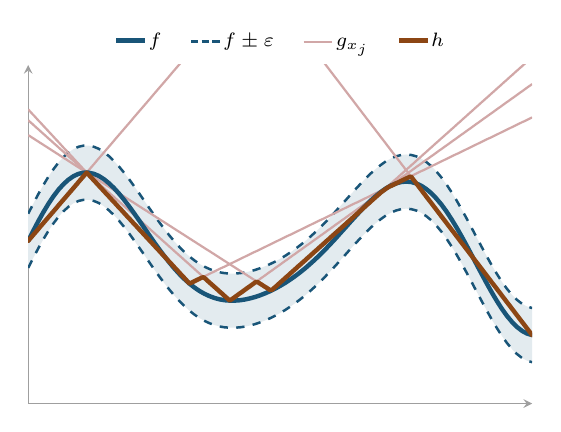
\begin{tikzpicture}
    \begin{axis}[swaxis, width=6.4cm, height=4.3cm, xmin=0, xmax=5, ymin=0.25, ymax=3.0,
        xtick=\empty, title={\scriptsize \textcolor{defcolor}{\rule[0.45ex]{1.3em}{1.6pt}}\,$f$ \quad \textcolor{defcolor}{\rule[0.45ex]{0.32em}{0.9pt}\,\rule[0.45ex]{0.32em}{0.9pt}\,\rule[0.45ex]{0.32em}{0.9pt}}\,$f \pm \varepsilon$ \quad \textcolor{thmcolor!40}{\rule[0.45ex]{1.3em}{0.8pt}}\,$g_{x_j}$ \quad \textcolor{mAccent}{\rule[0.45ex]{1.3em}{1.6pt}}\,$h$}, title style={yshift=-1.2ex, fill=white, fill opacity=0.6, text opacity=1, inner sep=2pt}, ytick=\empty]
      \addplot[draw=none, fill=defcolor!12] coordinates {(0.000,1.792) (0.050,1.873) (0.100,1.951) (0.150,2.024) (0.200,2.092) (0.250,2.153) (0.300,2.207) (0.350,2.252) (0.400,2.289) (0.450,2.317) (0.500,2.336) (0.550,2.345) (0.600,2.345) (0.650,2.336) (0.700,2.319) (0.750,2.293) (0.800,2.260) (0.850,2.221) (0.900,2.176) (0.950,2.126) (1.000,2.073) (1.050,2.016) (1.100,1.958) (1.150,1.899) (1.200,1.839) (1.250,1.780) (1.300,1.723) (1.350,1.668) (1.400,1.616) (1.450,1.567) (1.500,1.522) (1.550,1.481) (1.600,1.444) (1.650,1.412) (1.700,1.384) (1.750,1.361) (1.800,1.342) (1.850,1.327) (1.900,1.316) (1.950,1.309) (2.000,1.306) (2.050,1.306) (2.100,1.309) (2.150,1.315) (2.200,1.324) (2.250,1.335) (2.300,1.349) (2.350,1.365) (2.400,1.383) (2.450,1.403) (2.500,1.426) (2.550,1.450) (2.600,1.477) (2.650,1.506) (2.700,1.537) (2.750,1.570) (2.800,1.606) (2.850,1.643) (2.900,1.683) (2.950,1.724) (3.000,1.767) (3.050,1.811) (3.100,1.857) (3.150,1.902) (3.200,1.948) (3.250,1.993) (3.300,2.037) (3.350,2.080) (3.400,2.120) (3.450,2.156) (3.500,2.189) (3.550,2.218) (3.600,2.241) (3.650,2.258) (3.700,2.269) (3.750,2.273) (3.800,2.269) (3.850,2.258) (3.900,2.239) (3.950,2.212) (4.000,2.178) (4.050,2.135) (4.100,2.086) (4.150,2.030) (4.200,1.967) (4.250,1.900) (4.300,1.828) (4.350,1.753) (4.400,1.676) (4.450,1.598) (4.500,1.521) (4.550,1.445) (4.600,1.372) (4.650,1.303) (4.700,1.239) (4.750,1.182) (4.800,1.133) (4.850,1.092) (4.900,1.060) (4.950,1.038) (5.000,1.026) (5.000,0.586) (4.950,0.598) (4.900,0.620) (4.850,0.652) (4.800,0.693) (4.750,0.742) (4.700,0.799) (4.650,0.863) (4.600,0.932) (4.550,1.005) (4.500,1.081) (4.450,1.158) (4.400,1.236) (4.350,1.313) (4.300,1.388) (4.250,1.460) (4.200,1.527) (4.150,1.590) (4.100,1.646) (4.050,1.695) (4.000,1.738) (3.950,1.772) (3.900,1.799) (3.850,1.818) (3.800,1.829) (3.750,1.833) (3.700,1.829) (3.650,1.818) (3.600,1.801) (3.550,1.778) (3.500,1.749) (3.450,1.716) (3.400,1.680) (3.350,1.640) (3.300,1.597) (3.250,1.553) (3.200,1.508) (3.150,1.462) (3.100,1.417) (3.050,1.371) (3.000,1.327) (2.950,1.284) (2.900,1.243) (2.850,1.203) (2.800,1.166) (2.750,1.130) (2.700,1.097) (2.650,1.066) (2.600,1.037) (2.550,1.010) (2.500,0.986) (2.450,0.963) (2.400,0.943) (2.350,0.925) (2.300,0.909) (2.250,0.895) (2.200,0.884) (2.150,0.875) (2.100,0.869) (2.050,0.866) (2.000,0.866) (1.950,0.869) (1.900,0.876) (1.850,0.887) (1.800,0.902) (1.750,0.921) (1.700,0.944) (1.650,0.972) (1.600,1.004) (1.550,1.041) (1.500,1.082) (1.450,1.127) (1.400,1.176) (1.350,1.228) (1.300,1.283) (1.250,1.340) (1.200,1.399) (1.150,1.459) (1.100,1.518) (1.050,1.576) (1.000,1.633) (0.950,1.686) (0.900,1.736) (0.850,1.781) (0.800,1.820) (0.750,1.853) (0.700,1.879) (0.650,1.896) (0.600,1.905) (0.550,1.905) (0.500,1.896) (0.450,1.877) (0.400,1.849) (0.350,1.812) (0.300,1.767) (0.250,1.713) (0.200,1.652) (0.150,1.584) (0.100,1.511) (0.050,1.433) (0.000,1.352)} -- cycle;
      \addplot[defcolor, dashed, line width=0.9pt] coordinates {(0.000,1.792) (0.050,1.873) (0.100,1.951) (0.150,2.024) (0.200,2.092) (0.250,2.153) (0.300,2.207) (0.350,2.252) (0.400,2.289) (0.450,2.317) (0.500,2.336) (0.550,2.345) (0.600,2.345) (0.650,2.336) (0.700,2.319) (0.750,2.293) (0.800,2.260) (0.850,2.221) (0.900,2.176) (0.950,2.126) (1.000,2.073) (1.050,2.016) (1.100,1.958) (1.150,1.899) (1.200,1.839) (1.250,1.780) (1.300,1.723) (1.350,1.668) (1.400,1.616) (1.450,1.567) (1.500,1.522) (1.550,1.481) (1.600,1.444) (1.650,1.412) (1.700,1.384) (1.750,1.361) (1.800,1.342) (1.850,1.327) (1.900,1.316) (1.950,1.309) (2.000,1.306) (2.050,1.306) (2.100,1.309) (2.150,1.315) (2.200,1.324) (2.250,1.335) (2.300,1.349) (2.350,1.365) (2.400,1.383) (2.450,1.403) (2.500,1.426) (2.550,1.450) (2.600,1.477) (2.650,1.506) (2.700,1.537) (2.750,1.570) (2.800,1.606) (2.850,1.643) (2.900,1.683) (2.950,1.724) (3.000,1.767) (3.050,1.811) (3.100,1.857) (3.150,1.902) (3.200,1.948) (3.250,1.993) (3.300,2.037) (3.350,2.080) (3.400,2.120) (3.450,2.156) (3.500,2.189) (3.550,2.218) (3.600,2.241) (3.650,2.258) (3.700,2.269) (3.750,2.273) (3.800,2.269) (3.850,2.258) (3.900,2.239) (3.950,2.212) (4.000,2.178) (4.050,2.135) (4.100,2.086) (4.150,2.030) (4.200,1.967) (4.250,1.900) (4.300,1.828) (4.350,1.753) (4.400,1.676) (4.450,1.598) (4.500,1.521) (4.550,1.445) (4.600,1.372) (4.650,1.303) (4.700,1.239) (4.750,1.182) (4.800,1.133) (4.850,1.092) (4.900,1.060) (4.950,1.038) (5.000,1.026)};
      \addplot[defcolor, dashed, line width=0.9pt] coordinates {(0.000,1.352) (0.050,1.433) (0.100,1.511) (0.150,1.584) (0.200,1.652) (0.250,1.713) (0.300,1.767) (0.350,1.812) (0.400,1.849) (0.450,1.877) (0.500,1.896) (0.550,1.905) (0.600,1.905) (0.650,1.896) (0.700,1.879) (0.750,1.853) (0.800,1.820) (0.850,1.781) (0.900,1.736) (0.950,1.686) (1.000,1.633) (1.050,1.576) (1.100,1.518) (1.150,1.459) (1.200,1.399) (1.250,1.340) (1.300,1.283) (1.350,1.228) (1.400,1.176) (1.450,1.127) (1.500,1.082) (1.550,1.041) (1.600,1.004) (1.650,0.972) (1.700,0.944) (1.750,0.921) (1.800,0.902) (1.850,0.887) (1.900,0.876) (1.950,0.869) (2.000,0.866) (2.050,0.866) (2.100,0.869) (2.150,0.875) (2.200,0.884) (2.250,0.895) (2.300,0.909) (2.350,0.925) (2.400,0.943) (2.450,0.963) (2.500,0.986) (2.550,1.010) (2.600,1.037) (2.650,1.066) (2.700,1.097) (2.750,1.130) (2.800,1.166) (2.850,1.203) (2.900,1.243) (2.950,1.284) (3.000,1.327) (3.050,1.371) (3.100,1.417) (3.150,1.462) (3.200,1.508) (3.250,1.553) (3.300,1.597) (3.350,1.640) (3.400,1.680) (3.450,1.716) (3.500,1.749) (3.550,1.778) (3.600,1.801) (3.650,1.818) (3.700,1.829) (3.750,1.833) (3.800,1.829) (3.850,1.818) (3.900,1.799) (3.950,1.772) (4.000,1.738) (4.050,1.695) (4.100,1.646) (4.150,1.590) (4.200,1.527) (4.250,1.460) (4.300,1.388) (4.350,1.313) (4.400,1.236) (4.450,1.158) (4.500,1.081) (4.550,1.005) (4.600,0.932) (4.650,0.863) (4.700,0.799) (4.750,0.742) (4.800,0.693) (4.850,0.652) (4.900,0.620) (4.950,0.598) (5.000,0.586)};
      \addplot[thmcolor!40, line width=0.8pt] coordinates {(0.000,2.639) (0.020,2.621) (0.040,2.603) (0.060,2.586) (0.080,2.568) (0.100,2.550) (0.120,2.533) (0.140,2.515) (0.160,2.497) (0.180,2.480) (0.200,2.462) (0.220,2.444) (0.240,2.427) (0.260,2.409) (0.280,2.391) (0.300,2.374) (0.320,2.356) (0.340,2.338) (0.360,2.320) (0.380,2.303) (0.400,2.285) (0.420,2.267) (0.440,2.250) (0.460,2.232) (0.480,2.214) (0.500,2.197) (0.520,2.179) (0.540,2.161) (0.560,2.144) (0.580,2.126) (0.600,2.108) (0.620,2.091) (0.640,2.073) (0.660,2.055) (0.680,2.038) (0.700,2.020) (0.720,2.002) (0.740,1.985) (0.760,1.967) (0.780,1.949) (0.800,1.932) (0.820,1.914) (0.840,1.896) (0.860,1.879) (0.880,1.861) (0.900,1.843) (0.920,1.826) (0.940,1.808) (0.960,1.790) (0.980,1.772) (1.000,1.755) (1.020,1.737) (1.040,1.719) (1.060,1.702) (1.080,1.684) (1.100,1.666) (1.120,1.649) (1.140,1.631) (1.160,1.613) (1.180,1.596) (1.200,1.578) (1.220,1.560) (1.240,1.543) (1.260,1.525) (1.280,1.507) (1.300,1.490) (1.320,1.472) (1.340,1.454) (1.360,1.437) (1.380,1.419) (1.400,1.401) (1.420,1.384) (1.440,1.366) (1.460,1.348) (1.480,1.331) (1.500,1.313) (1.520,1.295) (1.540,1.278) (1.560,1.260) (1.580,1.242) (1.600,1.224) (1.620,1.232) (1.640,1.240) (1.660,1.248) (1.680,1.256) (1.700,1.264) (1.720,1.272) (1.740,1.280) (1.760,1.288) (1.780,1.296) (1.800,1.304) (1.820,1.312) (1.840,1.320) (1.860,1.328) (1.880,1.336) (1.900,1.344) (1.920,1.352) (1.940,1.359) (1.960,1.367) (1.980,1.375) (2.000,1.383) (2.020,1.391) (2.040,1.399) (2.060,1.407) (2.080,1.415) (2.100,1.423) (2.120,1.431) (2.140,1.439) (2.160,1.447) (2.180,1.455) (2.200,1.463) (2.220,1.471) (2.240,1.479) (2.260,1.486) (2.280,1.494) (2.300,1.502) (2.320,1.510) (2.340,1.518) (2.360,1.526) (2.380,1.534) (2.400,1.542) (2.420,1.550) (2.440,1.558) (2.460,1.566) (2.480,1.574) (2.500,1.582) (2.520,1.590) (2.540,1.598) (2.560,1.606) (2.580,1.614) (2.600,1.621) (2.620,1.629) (2.640,1.637) (2.660,1.645) (2.680,1.653) (2.700,1.661) (2.720,1.669) (2.740,1.677) (2.760,1.685) (2.780,1.693) (2.800,1.701) (2.820,1.709) (2.840,1.717) (2.860,1.725) (2.880,1.733) (2.900,1.741) (2.920,1.748) (2.940,1.756) (2.960,1.764) (2.980,1.772) (3.000,1.780) (3.020,1.788) (3.040,1.796) (3.060,1.804) (3.080,1.812) (3.100,1.820) (3.120,1.828) (3.140,1.836) (3.160,1.844) (3.180,1.852) (3.200,1.860) (3.220,1.868) (3.240,1.876) (3.260,1.883) (3.280,1.891) (3.300,1.899) (3.320,1.907) (3.340,1.915) (3.360,1.923) (3.380,1.931) (3.400,1.939) (3.420,1.947) (3.440,1.955) (3.460,1.963) (3.480,1.971) (3.500,1.979) (3.520,1.987) (3.540,1.995) (3.560,2.003) (3.580,2.011) (3.600,2.018) (3.620,2.026) (3.640,2.034) (3.660,2.042) (3.680,2.050) (3.700,2.058) (3.720,2.066) (3.740,2.074) (3.760,2.082) (3.780,2.090) (3.800,2.098) (3.820,2.106) (3.840,2.114) (3.860,2.122) (3.880,2.130) (3.900,2.138) (3.920,2.145) (3.940,2.153) (3.960,2.161) (3.980,2.169) (4.000,2.177) (4.020,2.185) (4.040,2.193) (4.060,2.201) (4.080,2.209) (4.100,2.217) (4.120,2.225) (4.140,2.233) (4.160,2.241) (4.180,2.249) (4.200,2.257) (4.220,2.265) (4.240,2.273) (4.260,2.280) (4.280,2.288) (4.300,2.296) (4.320,2.304) (4.340,2.312) (4.360,2.320) (4.380,2.328) (4.400,2.336) (4.420,2.344) (4.440,2.352) (4.460,2.360) (4.480,2.368) (4.500,2.376) (4.520,2.384) (4.540,2.392) (4.560,2.400) (4.580,2.407) (4.600,2.415) (4.620,2.423) (4.640,2.431) (4.660,2.439) (4.680,2.447) (4.700,2.455) (4.720,2.463) (4.740,2.471) (4.760,2.479) (4.780,2.487) (4.800,2.495) (4.820,2.503) (4.840,2.511) (4.860,2.519) (4.880,2.527) (4.900,2.535) (4.920,2.542) (4.940,2.550) (4.960,2.558) (4.980,2.566) (5.000,2.574)};
      \addplot[thmcolor!40, line width=0.8pt] coordinates {(0.000,6.165) (0.020,6.143) (0.040,6.122) (0.060,6.100) (0.080,6.079) (0.100,6.057) (0.120,6.036) (0.140,6.015) (0.160,5.993) (0.180,5.972) (0.200,5.950) (0.220,5.929) (0.240,5.907) (0.260,5.886) (0.280,5.864) (0.300,5.843) (0.320,5.822) (0.340,5.800) (0.360,5.779) (0.380,5.757) (0.400,5.736) (0.420,5.714) (0.440,5.693) (0.460,5.672) (0.480,5.650) (0.500,5.629) (0.520,5.607) (0.540,5.586) (0.560,5.564) (0.580,5.543) (0.600,5.522) (0.620,5.500) (0.640,5.479) (0.660,5.457) (0.680,5.436) (0.700,5.414) (0.720,5.393) (0.740,5.371) (0.760,5.350) (0.780,5.329) (0.800,5.307) (0.820,5.286) (0.840,5.264) (0.860,5.243) (0.880,5.221) (0.900,5.200) (0.920,5.179) (0.940,5.157) (0.960,5.136) (0.980,5.114) (1.000,5.093) (1.020,5.071) (1.040,5.050) (1.060,5.029) (1.080,5.007) (1.100,4.986) (1.120,4.964) (1.140,4.943) (1.160,4.921) (1.180,4.900) (1.200,4.878) (1.220,4.857) (1.240,4.836) (1.260,4.814) (1.280,4.793) (1.300,4.771) (1.320,4.750) (1.340,4.728) (1.360,4.707) (1.380,4.686) (1.400,4.664) (1.420,4.643) (1.440,4.621) (1.460,4.600) (1.480,4.578) (1.500,4.557) (1.520,4.536) (1.540,4.514) (1.560,4.493) (1.580,4.471) (1.600,4.450) (1.620,4.428) (1.640,4.407) (1.660,4.385) (1.680,4.364) (1.700,4.343) (1.720,4.321) (1.740,4.300) (1.760,4.278) (1.780,4.257) (1.800,4.235) (1.820,4.214) (1.840,4.193) (1.860,4.171) (1.880,4.150) (1.900,4.128) (1.920,4.107) (1.940,4.085) (1.960,4.064) (1.980,4.043) (2.000,4.021) (2.020,4.000) (2.040,3.978) (2.060,3.957) (2.080,3.935) (2.100,3.914) (2.120,3.892) (2.140,3.871) (2.160,3.850) (2.180,3.828) (2.200,3.807) (2.220,3.785) (2.240,3.764) (2.260,3.742) (2.280,3.721) (2.300,3.700) (2.320,3.678) (2.340,3.657) (2.360,3.635) (2.380,3.614) (2.400,3.592) (2.420,3.571) (2.440,3.549) (2.460,3.528) (2.480,3.507) (2.500,3.485) (2.520,3.464) (2.540,3.442) (2.560,3.421) (2.580,3.399) (2.600,3.378) (2.620,3.357) (2.640,3.335) (2.660,3.314) (2.680,3.292) (2.700,3.271) (2.720,3.249) (2.740,3.228) (2.760,3.207) (2.780,3.185) (2.800,3.164) (2.820,3.142) (2.840,3.121) (2.860,3.099) (2.880,3.078) (2.900,3.056) (2.920,3.035) (2.940,3.014) (2.960,2.992) (2.980,2.971) (3.000,2.949) (3.020,2.928) (3.040,2.906) (3.060,2.885) (3.080,2.864) (3.100,2.842) (3.120,2.821) (3.140,2.799) (3.160,2.778) (3.180,2.756) (3.200,2.735) (3.220,2.714) (3.240,2.692) (3.260,2.671) (3.280,2.649) (3.300,2.628) (3.320,2.606) (3.340,2.585) (3.360,2.563) (3.380,2.542) (3.400,2.521) (3.420,2.499) (3.440,2.478) (3.460,2.456) (3.480,2.435) (3.500,2.413) (3.520,2.392) (3.540,2.371) (3.560,2.349) (3.580,2.328) (3.600,2.306) (3.620,2.285) (3.640,2.263) (3.660,2.242) (3.680,2.221) (3.700,2.199) (3.720,2.178) (3.740,2.156) (3.760,2.135) (3.780,2.113) (3.800,2.092) (3.820,2.070) (3.840,2.049) (3.860,2.028) (3.880,2.006) (3.900,1.985) (3.920,1.963) (3.940,1.942) (3.960,1.920) (3.980,1.899) (4.000,1.878) (4.020,1.856) (4.040,1.835) (4.060,1.813) (4.080,1.792) (4.100,1.770) (4.120,1.749) (4.140,1.728) (4.160,1.706) (4.180,1.685) (4.200,1.663) (4.220,1.642) (4.240,1.620) (4.260,1.599) (4.280,1.577) (4.300,1.556) (4.320,1.535) (4.340,1.513) (4.360,1.492) (4.380,1.470) (4.400,1.449) (4.420,1.427) (4.440,1.406) (4.460,1.385) (4.480,1.363) (4.500,1.342) (4.520,1.320) (4.540,1.299) (4.560,1.277) (4.580,1.256) (4.600,1.234) (4.620,1.213) (4.640,1.192) (4.660,1.170) (4.680,1.149) (4.700,1.127) (4.720,1.106) (4.740,1.084) (4.760,1.063) (4.780,1.042) (4.800,1.020) (4.820,0.999) (4.840,0.977) (4.860,0.956) (4.880,0.934) (4.900,0.913) (4.920,0.892) (4.940,0.870) (4.960,0.849) (4.980,0.827) (5.000,0.806)};
      \addplot[thmcolor!40, line width=0.8pt] coordinates {(0.000,1.572) (0.020,1.591) (0.040,1.610) (0.060,1.629) (0.080,1.648) (0.100,1.667) (0.120,1.687) (0.140,1.706) (0.160,1.725) (0.180,1.744) (0.200,1.763) (0.220,1.782) (0.240,1.801) (0.260,1.820) (0.280,1.839) (0.300,1.859) (0.320,1.878) (0.340,1.897) (0.360,1.916) (0.380,1.935) (0.400,1.954) (0.420,1.973) (0.440,1.992) (0.460,2.011) (0.480,2.030) (0.500,2.050) (0.520,2.069) (0.540,2.088) (0.560,2.107) (0.580,2.126) (0.600,2.145) (0.620,2.164) (0.640,2.183) (0.660,2.202) (0.680,2.222) (0.700,2.241) (0.720,2.260) (0.740,2.279) (0.760,2.298) (0.780,2.317) (0.800,2.336) (0.820,2.355) (0.840,2.374) (0.860,2.394) (0.880,2.413) (0.900,2.432) (0.920,2.451) (0.940,2.470) (0.960,2.489) (0.980,2.508) (1.000,2.527) (1.020,2.546) (1.040,2.566) (1.060,2.585) (1.080,2.604) (1.100,2.623) (1.120,2.642) (1.140,2.661) (1.160,2.680) (1.180,2.699) (1.200,2.718) (1.220,2.737) (1.240,2.757) (1.260,2.776) (1.280,2.795) (1.300,2.814) (1.320,2.833) (1.340,2.852) (1.360,2.871) (1.380,2.890) (1.400,2.909) (1.420,2.929) (1.440,2.948) (1.460,2.967) (1.480,2.986) (1.500,3.005) (1.520,3.024) (1.540,3.043) (1.560,3.062) (1.580,3.081) (1.600,3.101) (1.620,3.120) (1.640,3.139) (1.660,3.158) (1.680,3.177) (1.700,3.196) (1.720,3.215) (1.740,3.234) (1.760,3.253) (1.780,3.272) (1.800,3.292) (1.820,3.311) (1.840,3.330) (1.860,3.349) (1.880,3.368) (1.900,3.387) (1.920,3.406) (1.940,3.425) (1.960,3.444) (1.980,3.464) (2.000,3.483) (2.020,3.502) (2.040,3.521) (2.060,3.540) (2.080,3.559) (2.100,3.578) (2.120,3.597) (2.140,3.616) (2.160,3.636) (2.180,3.655) (2.200,3.674) (2.220,3.693) (2.240,3.712) (2.260,3.731) (2.280,3.750) (2.300,3.769) (2.320,3.788) (2.340,3.808) (2.360,3.827) (2.380,3.846) (2.400,3.865) (2.420,3.884) (2.440,3.903) (2.460,3.922) (2.480,3.941) (2.500,3.960) (2.520,3.979) (2.540,3.999) (2.560,4.018) (2.580,4.037) (2.600,4.056) (2.620,4.075) (2.640,4.094) (2.660,4.113) (2.680,4.132) (2.700,4.151) (2.720,4.171) (2.740,4.190) (2.760,4.209) (2.780,4.228) (2.800,4.247) (2.820,4.266) (2.840,4.285) (2.860,4.304) (2.880,4.323) (2.900,4.343) (2.920,4.362) (2.940,4.381) (2.960,4.400) (2.980,4.419) (3.000,4.438) (3.020,4.457) (3.040,4.476) (3.060,4.495) (3.080,4.514) (3.100,4.534) (3.120,4.553) (3.140,4.572) (3.160,4.591) (3.180,4.610) (3.200,4.629) (3.220,4.648) (3.240,4.667) (3.260,4.686) (3.280,4.706) (3.300,4.725) (3.320,4.744) (3.340,4.763) (3.360,4.782) (3.380,4.801) (3.400,4.820) (3.420,4.839) (3.440,4.858) (3.460,4.878) (3.480,4.897) (3.500,4.916) (3.520,4.935) (3.540,4.954) (3.560,4.973) (3.580,4.992) (3.600,5.011) (3.620,5.030) (3.640,5.050) (3.660,5.069) (3.680,5.088) (3.700,5.107) (3.720,5.126) (3.740,5.145) (3.760,5.164) (3.780,5.183) (3.800,5.202) (3.820,5.221) (3.840,5.241) (3.860,5.260) (3.880,5.279) (3.900,5.298) (3.920,5.317) (3.940,5.336) (3.960,5.355) (3.980,5.374) (4.000,5.393) (4.020,5.413) (4.040,5.432) (4.060,5.451) (4.080,5.470) (4.100,5.489) (4.120,5.508) (4.140,5.527) (4.160,5.546) (4.180,5.565) (4.200,5.585) (4.220,5.604) (4.240,5.623) (4.260,5.642) (4.280,5.661) (4.300,5.680) (4.320,5.699) (4.340,5.718) (4.360,5.737) (4.380,5.756) (4.400,5.776) (4.420,5.795) (4.440,5.814) (4.460,5.833) (4.480,5.852) (4.500,5.871) (4.520,5.890) (4.540,5.909) (4.560,5.928) (4.580,5.948) (4.600,5.967) (4.620,5.986) (4.640,6.005) (4.660,6.024) (4.680,6.043) (4.700,6.062) (4.720,6.081) (4.740,6.100) (4.760,6.120) (4.780,6.139) (4.800,6.158) (4.820,6.177) (4.840,6.196) (4.860,6.215) (4.880,6.234) (4.900,6.253) (4.920,6.272) (4.940,6.291) (4.960,6.311) (4.980,6.330) (5.000,6.349)};
      \addplot[thmcolor!40, line width=0.8pt] coordinates {(0.000,2.430) (0.020,2.420) (0.040,2.409) (0.060,2.399) (0.080,2.388) (0.100,2.378) (0.120,2.367) (0.140,2.357) (0.160,2.346) (0.180,2.336) (0.200,2.325) (0.220,2.315) (0.240,2.304) (0.260,2.294) (0.280,2.283) (0.300,2.273) (0.320,2.262) (0.340,2.252) (0.360,2.241) (0.380,2.231) (0.400,2.220) (0.420,2.210) (0.440,2.199) (0.460,2.189) (0.480,2.178) (0.500,2.168) (0.520,2.157) (0.540,2.147) (0.560,2.137) (0.580,2.126) (0.600,2.116) (0.620,2.105) (0.640,2.095) (0.660,2.084) (0.680,2.074) (0.700,2.063) (0.720,2.053) (0.740,2.042) (0.760,2.032) (0.780,2.021) (0.800,2.011) (0.820,2.000) (0.840,1.990) (0.860,1.979) (0.880,1.969) (0.900,1.958) (0.920,1.948) (0.940,1.937) (0.960,1.927) (0.980,1.916) (1.000,1.906) (1.020,1.895) (1.040,1.885) (1.060,1.874) (1.080,1.864) (1.100,1.853) (1.120,1.843) (1.140,1.832) (1.160,1.822) (1.180,1.812) (1.200,1.801) (1.220,1.791) (1.240,1.780) (1.260,1.770) (1.280,1.759) (1.300,1.749) (1.320,1.738) (1.340,1.728) (1.360,1.717) (1.380,1.707) (1.400,1.696) (1.420,1.686) (1.440,1.675) (1.460,1.665) (1.480,1.654) (1.500,1.644) (1.520,1.633) (1.540,1.623) (1.560,1.612) (1.580,1.602) (1.600,1.591) (1.620,1.581) (1.640,1.570) (1.660,1.560) (1.680,1.549) (1.700,1.539) (1.720,1.528) (1.740,1.518) (1.760,1.507) (1.780,1.497) (1.800,1.487) (1.820,1.476) (1.840,1.466) (1.860,1.455) (1.880,1.445) (1.900,1.434) (1.920,1.424) (1.940,1.413) (1.960,1.403) (1.980,1.392) (2.000,1.382) (2.020,1.371) (2.040,1.361) (2.060,1.350) (2.080,1.340) (2.100,1.329) (2.120,1.319) (2.140,1.308) (2.160,1.298) (2.180,1.287) (2.200,1.277) (2.220,1.266) (2.240,1.256) (2.260,1.245) (2.280,1.235) (2.300,1.224) (2.320,1.214) (2.340,1.203) (2.360,1.193) (2.380,1.182) (2.400,1.172) (2.420,1.174) (2.440,1.189) (2.460,1.203) (2.480,1.218) (2.500,1.233) (2.520,1.247) (2.540,1.262) (2.560,1.277) (2.580,1.291) (2.600,1.306) (2.620,1.321) (2.640,1.335) (2.660,1.350) (2.680,1.365) (2.700,1.379) (2.720,1.394) (2.740,1.408) (2.760,1.423) (2.780,1.438) (2.800,1.452) (2.820,1.467) (2.840,1.482) (2.860,1.496) (2.880,1.511) (2.900,1.526) (2.920,1.540) (2.940,1.555) (2.960,1.570) (2.980,1.584) (3.000,1.599) (3.020,1.614) (3.040,1.628) (3.060,1.643) (3.080,1.657) (3.100,1.672) (3.120,1.687) (3.140,1.701) (3.160,1.716) (3.180,1.731) (3.200,1.745) (3.220,1.760) (3.240,1.775) (3.260,1.789) (3.280,1.804) (3.300,1.819) (3.320,1.833) (3.340,1.848) (3.360,1.863) (3.380,1.877) (3.400,1.892) (3.420,1.907) (3.440,1.921) (3.460,1.936) (3.480,1.950) (3.500,1.965) (3.520,1.980) (3.540,1.994) (3.560,2.009) (3.580,2.024) (3.600,2.038) (3.620,2.053) (3.640,2.068) (3.660,2.082) (3.680,2.097) (3.700,2.112) (3.720,2.126) (3.740,2.141) (3.760,2.156) (3.780,2.170) (3.800,2.185) (3.820,2.199) (3.840,2.214) (3.860,2.229) (3.880,2.243) (3.900,2.258) (3.920,2.273) (3.940,2.287) (3.960,2.302) (3.980,2.317) (4.000,2.331) (4.020,2.346) (4.040,2.361) (4.060,2.375) (4.080,2.390) (4.100,2.405) (4.120,2.419) (4.140,2.434) (4.160,2.448) (4.180,2.463) (4.200,2.478) (4.220,2.492) (4.240,2.507) (4.260,2.522) (4.280,2.536) (4.300,2.551) (4.320,2.566) (4.340,2.580) (4.360,2.595) (4.380,2.610) (4.400,2.624) (4.420,2.639) (4.440,2.654) (4.460,2.668) (4.480,2.683) (4.500,2.698) (4.520,2.712) (4.540,2.727) (4.560,2.741) (4.580,2.756) (4.600,2.771) (4.620,2.785) (4.640,2.800) (4.660,2.815) (4.680,2.829) (4.700,2.844) (4.720,2.859) (4.740,2.873) (4.760,2.888) (4.780,2.903) (4.800,2.917) (4.820,2.932) (4.840,2.947) (4.860,2.961) (4.880,2.976) (4.900,2.990) (4.920,3.005) (4.940,3.020) (4.960,3.034) (4.980,3.049) (5.000,3.064)};
      \addplot[thmcolor!40, line width=0.8pt] coordinates {(0.000,2.551) (0.020,2.536) (0.040,2.522) (0.060,2.507) (0.080,2.492) (0.100,2.478) (0.120,2.463) (0.140,2.448) (0.160,2.434) (0.180,2.419) (0.200,2.404) (0.220,2.390) (0.240,2.375) (0.260,2.360) (0.280,2.346) (0.300,2.331) (0.320,2.316) (0.340,2.302) (0.360,2.287) (0.380,2.273) (0.400,2.258) (0.420,2.243) (0.440,2.229) (0.460,2.214) (0.480,2.199) (0.500,2.185) (0.520,2.170) (0.540,2.155) (0.560,2.141) (0.580,2.126) (0.600,2.111) (0.620,2.097) (0.640,2.082) (0.660,2.067) (0.680,2.053) (0.700,2.038) (0.720,2.023) (0.740,2.009) (0.760,1.994) (0.780,1.980) (0.800,1.965) (0.820,1.950) (0.840,1.936) (0.860,1.921) (0.880,1.906) (0.900,1.892) (0.920,1.877) (0.940,1.862) (0.960,1.848) (0.980,1.833) (1.000,1.818) (1.020,1.804) (1.040,1.789) (1.060,1.774) (1.080,1.760) (1.100,1.745) (1.120,1.731) (1.140,1.716) (1.160,1.701) (1.180,1.687) (1.200,1.672) (1.220,1.657) (1.240,1.643) (1.260,1.628) (1.280,1.613) (1.300,1.599) (1.320,1.584) (1.340,1.569) (1.360,1.555) (1.380,1.540) (1.400,1.525) (1.420,1.511) (1.440,1.496) (1.460,1.481) (1.480,1.467) (1.500,1.452) (1.520,1.438) (1.540,1.423) (1.560,1.408) (1.580,1.394) (1.600,1.379) (1.620,1.364) (1.640,1.350) (1.660,1.335) (1.680,1.320) (1.700,1.306) (1.720,1.291) (1.740,1.276) (1.760,1.262) (1.780,1.247) (1.800,1.232) (1.820,1.218) (1.840,1.203) (1.860,1.189) (1.880,1.174) (1.900,1.159) (1.920,1.145) (1.940,1.130) (1.960,1.115) (1.980,1.101) (2.000,1.086) (2.020,1.098) (2.040,1.109) (2.060,1.121) (2.080,1.133) (2.100,1.145) (2.120,1.156) (2.140,1.168) (2.160,1.180) (2.180,1.192) (2.200,1.203) (2.220,1.215) (2.240,1.227) (2.260,1.238) (2.280,1.250) (2.300,1.262) (2.320,1.274) (2.340,1.285) (2.360,1.297) (2.380,1.309) (2.400,1.321) (2.420,1.332) (2.440,1.344) (2.460,1.356) (2.480,1.367) (2.500,1.379) (2.520,1.391) (2.540,1.403) (2.560,1.414) (2.580,1.426) (2.600,1.438) (2.620,1.450) (2.640,1.461) (2.660,1.473) (2.680,1.485) (2.700,1.496) (2.720,1.508) (2.740,1.520) (2.760,1.532) (2.780,1.543) (2.800,1.555) (2.820,1.567) (2.840,1.579) (2.860,1.590) (2.880,1.602) (2.900,1.614) (2.920,1.625) (2.940,1.637) (2.960,1.649) (2.980,1.661) (3.000,1.672) (3.020,1.684) (3.040,1.696) (3.060,1.708) (3.080,1.719) (3.100,1.731) (3.120,1.743) (3.140,1.754) (3.160,1.766) (3.180,1.778) (3.200,1.790) (3.220,1.801) (3.240,1.813) (3.260,1.825) (3.280,1.837) (3.300,1.848) (3.320,1.860) (3.340,1.872) (3.360,1.883) (3.380,1.895) (3.400,1.907) (3.420,1.919) (3.440,1.930) (3.460,1.942) (3.480,1.954) (3.500,1.966) (3.520,1.977) (3.540,1.989) (3.560,2.001) (3.580,2.012) (3.600,2.024) (3.620,2.036) (3.640,2.048) (3.660,2.059) (3.680,2.071) (3.700,2.083) (3.720,2.095) (3.740,2.106) (3.760,2.118) (3.780,2.130) (3.800,2.141) (3.820,2.153) (3.840,2.165) (3.860,2.177) (3.880,2.188) (3.900,2.200) (3.920,2.212) (3.940,2.224) (3.960,2.235) (3.980,2.247) (4.000,2.259) (4.020,2.270) (4.040,2.282) (4.060,2.294) (4.080,2.306) (4.100,2.317) (4.120,2.329) (4.140,2.341) (4.160,2.352) (4.180,2.364) (4.200,2.376) (4.220,2.388) (4.240,2.399) (4.260,2.411) (4.280,2.423) (4.300,2.435) (4.320,2.446) (4.340,2.458) (4.360,2.470) (4.380,2.481) (4.400,2.493) (4.420,2.505) (4.440,2.517) (4.460,2.528) (4.480,2.540) (4.500,2.552) (4.520,2.564) (4.540,2.575) (4.560,2.587) (4.580,2.599) (4.600,2.610) (4.620,2.622) (4.640,2.634) (4.660,2.646) (4.680,2.657) (4.700,2.669) (4.720,2.681) (4.740,2.693) (4.760,2.704) (4.780,2.716) (4.800,2.728) (4.820,2.739) (4.840,2.751) (4.860,2.763) (4.880,2.775) (4.900,2.786) (4.920,2.798) (4.940,2.810) (4.960,2.822) (4.980,2.833) (5.000,2.845)};
      \addplot[defcolor, curveln] coordinates {(0.000,1.572) (0.050,1.653) (0.100,1.731) (0.150,1.804) (0.200,1.872) (0.250,1.933) (0.300,1.987) (0.350,2.032) (0.400,2.069) (0.450,2.097) (0.500,2.116) (0.550,2.125) (0.600,2.125) (0.650,2.116) (0.700,2.099) (0.750,2.073) (0.800,2.040) (0.850,2.001) (0.900,1.956) (0.950,1.906) (1.000,1.853) (1.050,1.796) (1.100,1.738) (1.150,1.679) (1.200,1.619) (1.250,1.560) (1.300,1.503) (1.350,1.448) (1.400,1.396) (1.450,1.347) (1.500,1.302) (1.550,1.261) (1.600,1.224) (1.650,1.192) (1.700,1.164) (1.750,1.141) (1.800,1.122) (1.850,1.107) (1.900,1.096) (1.950,1.089) (2.000,1.086) (2.050,1.086) (2.100,1.089) (2.150,1.095) (2.200,1.104) (2.250,1.115) (2.300,1.129) (2.350,1.145) (2.400,1.163) (2.450,1.183) (2.500,1.206) (2.550,1.230) (2.600,1.257) (2.650,1.286) (2.700,1.317) (2.750,1.350) (2.800,1.386) (2.850,1.423) (2.900,1.463) (2.950,1.504) (3.000,1.547) (3.050,1.591) (3.100,1.637) (3.150,1.682) (3.200,1.728) (3.250,1.773) (3.300,1.817) (3.350,1.860) (3.400,1.900) (3.450,1.936) (3.500,1.969) (3.550,1.998) (3.600,2.021) (3.650,2.038) (3.700,2.049) (3.750,2.053) (3.800,2.049) (3.850,2.038) (3.900,2.019) (3.950,1.992) (4.000,1.958) (4.050,1.915) (4.100,1.866) (4.150,1.810) (4.200,1.747) (4.250,1.680) (4.300,1.608) (4.350,1.533) (4.400,1.456) (4.450,1.378) (4.500,1.301) (4.550,1.225) (4.600,1.152) (4.650,1.083) (4.700,1.019) (4.750,0.962) (4.800,0.913) (4.850,0.872) (4.900,0.840) (4.950,0.818) (5.000,0.806)};
      \addplot[mAccent, curveln] coordinates {(0.000,1.572) (0.020,1.591) (0.040,1.610) (0.060,1.629) (0.080,1.648) (0.100,1.667) (0.120,1.687) (0.140,1.706) (0.160,1.725) (0.180,1.744) (0.200,1.763) (0.220,1.782) (0.240,1.801) (0.260,1.820) (0.280,1.839) (0.300,1.859) (0.320,1.878) (0.340,1.897) (0.360,1.916) (0.380,1.935) (0.400,1.954) (0.420,1.973) (0.440,1.992) (0.460,2.011) (0.480,2.030) (0.500,2.050) (0.520,2.069) (0.540,2.088) (0.560,2.107) (0.580,2.126) (0.600,2.108) (0.620,2.091) (0.640,2.073) (0.660,2.055) (0.680,2.038) (0.700,2.020) (0.720,2.002) (0.740,1.985) (0.760,1.967) (0.780,1.949) (0.800,1.932) (0.820,1.914) (0.840,1.896) (0.860,1.879) (0.880,1.861) (0.900,1.843) (0.920,1.826) (0.940,1.808) (0.960,1.790) (0.980,1.772) (1.000,1.755) (1.020,1.737) (1.040,1.719) (1.060,1.702) (1.080,1.684) (1.100,1.666) (1.120,1.649) (1.140,1.631) (1.160,1.613) (1.180,1.596) (1.200,1.578) (1.220,1.560) (1.240,1.543) (1.260,1.525) (1.280,1.507) (1.300,1.490) (1.320,1.472) (1.340,1.454) (1.360,1.437) (1.380,1.419) (1.400,1.401) (1.420,1.384) (1.440,1.366) (1.460,1.348) (1.480,1.331) (1.500,1.313) (1.520,1.295) (1.540,1.278) (1.560,1.260) (1.580,1.242) (1.600,1.224) (1.620,1.232) (1.640,1.240) (1.660,1.248) (1.680,1.256) (1.700,1.264) (1.720,1.272) (1.740,1.276) (1.760,1.262) (1.780,1.247) (1.800,1.232) (1.820,1.218) (1.840,1.203) (1.860,1.189) (1.880,1.174) (1.900,1.159) (1.920,1.145) (1.940,1.130) (1.960,1.115) (1.980,1.101) (2.000,1.086) (2.020,1.098) (2.040,1.109) (2.060,1.121) (2.080,1.133) (2.100,1.145) (2.120,1.156) (2.140,1.168) (2.160,1.180) (2.180,1.192) (2.200,1.203) (2.220,1.215) (2.240,1.227) (2.260,1.238) (2.280,1.235) (2.300,1.224) (2.320,1.214) (2.340,1.203) (2.360,1.193) (2.380,1.182) (2.400,1.172) (2.420,1.174) (2.440,1.189) (2.460,1.203) (2.480,1.218) (2.500,1.233) (2.520,1.247) (2.540,1.262) (2.560,1.277) (2.580,1.291) (2.600,1.306) (2.620,1.321) (2.640,1.335) (2.660,1.350) (2.680,1.365) (2.700,1.379) (2.720,1.394) (2.740,1.408) (2.760,1.423) (2.780,1.438) (2.800,1.452) (2.820,1.467) (2.840,1.482) (2.860,1.496) (2.880,1.511) (2.900,1.526) (2.920,1.540) (2.940,1.555) (2.960,1.570) (2.980,1.584) (3.000,1.599) (3.020,1.614) (3.040,1.628) (3.060,1.643) (3.080,1.657) (3.100,1.672) (3.120,1.687) (3.140,1.701) (3.160,1.716) (3.180,1.731) (3.200,1.745) (3.220,1.760) (3.240,1.775) (3.260,1.789) (3.280,1.804) (3.300,1.819) (3.320,1.833) (3.340,1.848) (3.360,1.863) (3.380,1.877) (3.400,1.892) (3.420,1.907) (3.440,1.921) (3.460,1.936) (3.480,1.950) (3.500,1.965) (3.520,1.977) (3.540,1.989) (3.560,2.001) (3.580,2.011) (3.600,2.018) (3.620,2.026) (3.640,2.034) (3.660,2.042) (3.680,2.050) (3.700,2.058) (3.720,2.066) (3.740,2.074) (3.760,2.082) (3.780,2.090) (3.800,2.092) (3.820,2.070) (3.840,2.049) (3.860,2.028) (3.880,2.006) (3.900,1.985) (3.920,1.963) (3.940,1.942) (3.960,1.920) (3.980,1.899) (4.000,1.878) (4.020,1.856) (4.040,1.835) (4.060,1.813) (4.080,1.792) (4.100,1.770) (4.120,1.749) (4.140,1.728) (4.160,1.706) (4.180,1.685) (4.200,1.663) (4.220,1.642) (4.240,1.620) (4.260,1.599) (4.280,1.577) (4.300,1.556) (4.320,1.535) (4.340,1.513) (4.360,1.492) (4.380,1.470) (4.400,1.449) (4.420,1.427) (4.440,1.406) (4.460,1.385) (4.480,1.363) (4.500,1.342) (4.520,1.320) (4.540,1.299) (4.560,1.277) (4.580,1.256) (4.600,1.234) (4.620,1.213) (4.640,1.192) (4.660,1.170) (4.680,1.149) (4.700,1.127) (4.720,1.106) (4.740,1.084) (4.760,1.063) (4.780,1.042) (4.800,1.020) (4.820,0.999) (4.840,0.977) (4.860,0.956) (4.880,0.934) (4.900,0.913) (4.920,0.892) (4.940,0.870) (4.960,0.849) (4.980,0.827) (5.000,0.806)};
    \end{axis}
  \end{tikzpicture}
    \end{column}
  \end{columns}

  \note{
    It remains to check both sides. Every one of the functions satisfies
    equation 54, so each is above "f" minus epsilon everywhere, and
    therefore so is their minimum. That is equation 61. For the upper bound,
    any point "t" lies in one of the covering sets, where the corresponding
    function is below "f" plus epsilon, and the minimum is no larger. That
    is equation 62. Together they say that "h" is within epsilon of "f" on
    all of capital "K", which is equation 58. In the picture, the brown
    curve indeed stays inside the tube. Stone's theorem is proved.
  }
\end{frame}
}

{
\usebackgroundtemplate{%
  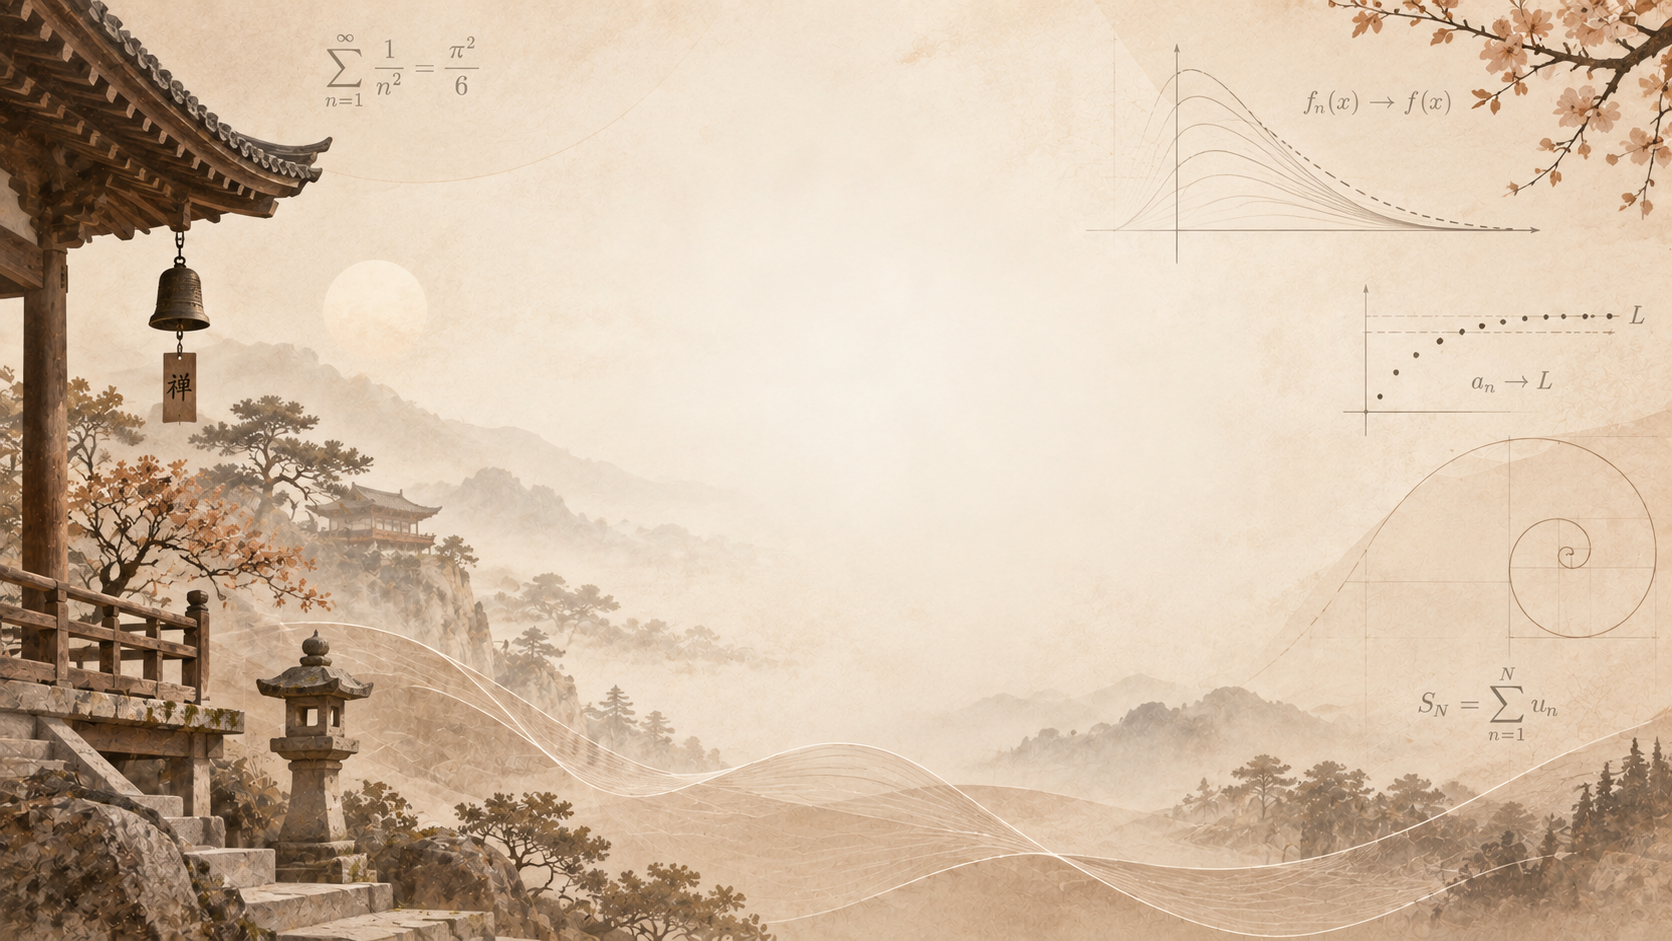
\includegraphics[width=\paperwidth,height=\paperheight,keepaspectratio=false]{chapter_07_bg_08.png}%
}
\section{Complex Algebras}

% --- Build 1/2 ---
\begin{frame}{Beyond Real Algebras}
  \begin{remblock}{Remark}
    Theorem 7.32 does \alert{not} hold for complex algebras. A counterexample is given in
    Exercise 21.
  \end{remblock}

  \vspace{0.3em}
  \begin{hlbox}
  \small On the unit circle, the polynomials in $e^{i\theta}$ separate points and vanish at no
  point --- yet they cannot approximate $e^{-i\theta}$.
  \end{hlbox}

  \note{
    Does the theorem hold for algebras of complex functions? As stated, it
    does not. Rudin gives a counterexample in Exercise 21. Here is the idea.
    On the unit circle, consider all polynomials in the complex exponential
    "e" to the power "i" theta. This algebra separates points and vanishes
    at no point. But every member, multiplied by that same exponential and
    integrated around the circle, gives zero, and this property passes to
    uniform limits. The conjugate function, "e" to the power minus "i"
    theta, does not have it. So it is continuous but not in the closure.
  }
\end{frame}

% --- Build 2/2 ---
\begin{frame}{Beyond Real Algebras}
  \begin{remblock}{Remark}
    Theorem 7.32 does \alert{not} hold for complex algebras. A counterexample is given in
    Exercise 21.
  \end{remblock}

  \vspace{0.3em}
  \begin{hlbox}
  \small On the unit circle, the polynomials in $e^{i\theta}$ separate points and vanish at no
  point --- yet they cannot approximate $e^{-i\theta}$.
  \end{hlbox}

  \vspace{0.7em}
  \begin{defblock}{Self-adjoint algebras}
    An algebra $\mathscr{A}$ of complex functions is \alert{self-adjoint} if for every
    $f \in \mathscr{A}$ its complex conjugate $\bar{f}$ also belongs to $\mathscr{A}$, where
    $\bar{f}(x) = \overline{f(x)}$.
  \end{defblock}

  \note{
    What went wrong? The real proof used absolute values, maximum, and
    minimum, which make no sense for complex functions. The remedy is one
    extra condition. An algebra of complex functions is called self-adjoint
    if it is closed under complex conjugation: whenever "f" is in the
    algebra, so is its conjugate, the function whose value at each point is
    the complex conjugate of the value of "f". The algebra in the
    counterexample fails this, since it lacks the conjugate of its own
    generator. With this condition added, the conclusion of Stone's theorem
    does hold.
  }
\end{frame}

% --- Build 1/2 ---
\begin{frame}{Theorem 7.33: The Complex Stone--Weierstrass Theorem}
  \begin{thmblock}{Theorem 7.33}
    Suppose $\mathscr{A}$ is a self-adjoint algebra of complex continuous functions on a
    compact set $K$, $\mathscr{A}$ separates points on $K$, and $\mathscr{A}$ vanishes at no point
    of $K$. Then the uniform closure $\mathscr{B}$ of $\mathscr{A}$ consists of all complex
    continuous functions on $K$.

    \medskip
    In other words, $\mathscr{A}$ is \alert{dense} in $\mathscr{C}(K)$.
  \end{thmblock}

  \note{
    Here is the complex version, Theorem 7.33. Let capital "A" be a
    self-adjoint algebra of complex continuous functions on a compact set
    capital "K", and assume, as before, that it separates points and
    vanishes at no point. Then its uniform closure is the set of all complex
    continuous functions on capital "K". In the language of metric spaces,
    capital "A" is dense in the space of continuous complex functions on
    capital "K" with the supremum metric, which we introduced in Definition
    7.14.
  }
\end{frame}

% --- Build 2/2 ---
\begin{frame}{Theorem 7.33: The Complex Stone--Weierstrass Theorem}
  \begin{thmblock}{Theorem 7.33}
    Suppose $\mathscr{A}$ is a self-adjoint algebra of complex continuous functions on a
    compact set $K$, $\mathscr{A}$ separates points on $K$, and $\mathscr{A}$ vanishes at no point
    of $K$. Then the uniform closure $\mathscr{B}$ of $\mathscr{A}$ consists of all complex
    continuous functions on $K$.

    \medskip
    In other words, $\mathscr{A}$ is \alert{dense} in $\mathscr{C}(K)$.
  \end{thmblock}
  \vspace{0.8em}
  \hl{\textbf{Strategy:} reduce to Theorem 7.32 by passing to the \emph{real} functions in $\mathscr{A}$.}

  \note{
    The strategy is to reduce to the real theorem. We look at the real
    valued functions inside capital "A", show that they form a real algebra
    satisfying the hypotheses of Theorem 7.32, and then reassemble complex
    functions from their real and imaginary parts. Let's carry this out.
  }
\end{frame}

% --- Build 1/4 ---
\begin{frame}{Proof of Theorem 7.33}
  \small
  \hl{Let $\mathscr{A}_R$ be the set of all \emph{real} functions on $K$ which belong to $\mathscr{A}$.}

  \vspace{0.1em}
  \begin{proofblock}{Proof}
    \begin{enumerate}\setlength{\itemsep}{0.05em}
      \item \textbf{Real parts.} If $f = u + iv \in \mathscr{A}$ with $u$, $v$ real, then
        $2u = f + \bar{f}$, so $u \in \mathscr{A}_R$.
    \end{enumerate}
  \end{proofblock}

  \note{
    Let capital "A" sub capital "R" denote the set of real valued members of
    capital "A". It is a real algebra. The first observation is that real
    parts of members stay in the algebra. Write a member "f" as "u" plus "i"
    times "v", with "u" and "v" real. Then "f" plus its conjugate equals 2
    times "u". Since capital "A" is self-adjoint, the conjugate is in
    capital "A", so "u" is in capital "A", and being real it lies in capital
    "A" sub capital "R". This is the only place where self-adjointness is
    used.
  }
\end{frame}

% --- Build 2/4 ---
\begin{frame}{Proof of Theorem 7.33}
  \small
  \hl{Let $\mathscr{A}_R$ be the set of all \emph{real} functions on $K$ which belong to $\mathscr{A}$.}

  \vspace{0.1em}
  \begin{proofblock}{Proof}
    \begin{enumerate}\setlength{\itemsep}{0.05em}
      \item \textbf{Real parts.} If $f = u + iv \in \mathscr{A}$ with $u$, $v$ real, then
        $2u = f + \bar{f}$, so $u \in \mathscr{A}_R$.
      \item \textbf{$\mathscr{A}_R$ separates points.} If $x_1 \ne x_2$, Theorem 7.31 gives
        $f \in \mathscr{A}$ with $f(x_1) = 1$, $f(x_2) = 0$. Hence $0 = u(x_2) \ne u(x_1) = 1$.
    \end{enumerate}
  \end{proofblock}

  \note{
    Next, the real algebra separates points. Given two distinct points,
    Theorem 7.31 provides a member "f" of capital "A" with value 1 at the
    first point and 0 at the second. Its real part "u" then also has the
    values 1 and 0 at these points, and "u" belongs to the real algebra by
    the first observation. So the real algebra can tell the two points
    apart.
  }
\end{frame}

% --- Build 3/4 ---
\begin{frame}{Proof of Theorem 7.33}
  \small
  \hl{Let $\mathscr{A}_R$ be the set of all \emph{real} functions on $K$ which belong to $\mathscr{A}$.}

  \vspace{0.1em}
  \begin{proofblock}{Proof}
    \begin{enumerate}\setlength{\itemsep}{0.05em}
      \item \textbf{Real parts.} If $f = u + iv \in \mathscr{A}$ with $u$, $v$ real, then
        $2u = f + \bar{f}$, so $u \in \mathscr{A}_R$.
      \item \textbf{$\mathscr{A}_R$ separates points.} If $x_1 \ne x_2$, Theorem 7.31 gives
        $f \in \mathscr{A}$ with $f(x_1) = 1$, $f(x_2) = 0$. Hence $0 = u(x_2) \ne u(x_1) = 1$.
      \item \textbf{$\mathscr{A}_R$ vanishes at no point.} If $x \in K$, then $g(x) \ne 0$ for some
        $g \in \mathscr{A}$; choose $\lambda$ with $\lambda g(x) > 0$. If
        $f = \lambda g = u + iv$, then $u(x) > 0$.
    \end{enumerate}
  \end{proofblock}

  \note{
    Third, the real algebra vanishes at no point. Given a point "x", some
    member "g" of capital "A" is nonzero there. The value "g" of "x" is a
    nonzero complex number, so we can rotate it onto the positive real axis:
    there is a complex number lambda such that lambda times "g" of "x" is
    positive. The function lambda times "g" is in capital "A", and its real
    part "u" is positive at "x". So the real algebra contains a function
    that is nonzero at "x".
  }
\end{frame}

% --- Build 4/4 ---
\begin{frame}{Proof of Theorem 7.33}
  \small
  \hl{Let $\mathscr{A}_R$ be the set of all \emph{real} functions on $K$ which belong to $\mathscr{A}$.}

  \vspace{0.1em}
  \begin{proofblock}{Proof}
    \begin{enumerate}\setlength{\itemsep}{0.05em}
      \item \textbf{Real parts.} If $f = u + iv \in \mathscr{A}$ with $u$, $v$ real, then
        $2u = f + \bar{f}$, so $u \in \mathscr{A}_R$.
      \item \textbf{$\mathscr{A}_R$ separates points.} If $x_1 \ne x_2$, Theorem 7.31 gives
        $f \in \mathscr{A}$ with $f(x_1) = 1$, $f(x_2) = 0$. Hence $0 = u(x_2) \ne u(x_1) = 1$.
      \item \textbf{$\mathscr{A}_R$ vanishes at no point.} If $x \in K$, then $g(x) \ne 0$ for some
        $g \in \mathscr{A}$; choose $\lambda$ with $\lambda g(x) > 0$. If
        $f = \lambda g = u + iv$, then $u(x) > 0$.
      \item \textbf{Conclusion.} By Theorem 7.32, every real continuous function on $K$ lies in
        the uniform closure of $\mathscr{A}_R$, hence in $\mathscr{B}$. If $f = u + iv$ is
        continuous, then $u, v \in \mathscr{B}$, hence $f \in \mathscr{B}$.
        \hfill $\blacksquare$
    \end{enumerate}
  \end{proofblock}

  \note{
    So the real algebra satisfies all hypotheses of Theorem 7.32. Therefore
    every real continuous function on capital "K" is in its uniform closure,
    and hence in capital "B". Finally, take any complex continuous function
    "f" and split it into real and imaginary parts, "u" and "v". Both are
    real and continuous, so both are in capital "B". Since capital "B" is a
    complex algebra, "u" plus "i" times "v" is in capital "B" as well. This
    completes the proof.
  }
\end{frame}
}

{
\usebackgroundtemplate{%
  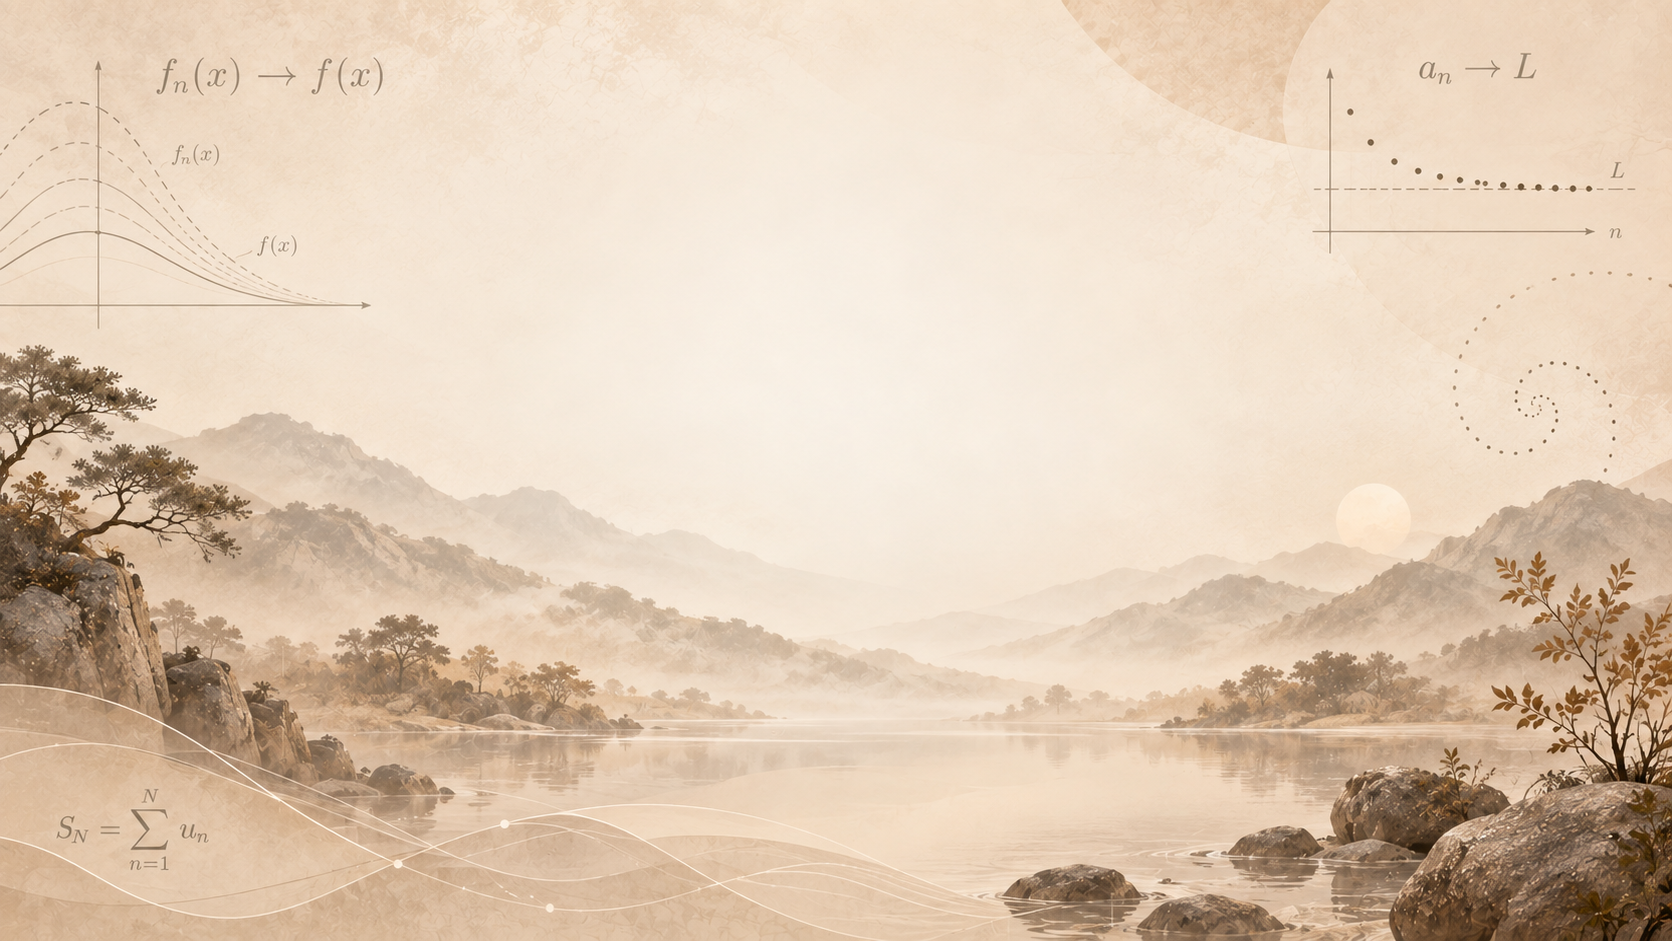
\includegraphics[width=\paperwidth,height=\paperheight,keepaspectratio=false]{chapter_07_bg_09.png}%
}
\section{Summary}

% --- Build 1/4 ---
\begin{frame}{Summary}
  \begin{hlbox}
  \textbf{Key takeaways from this section:}
  \begin{itemize}\setlength{\itemsep}{0.35em}
    \item \textbf{Weierstrass (7.26):} every continuous $f$ on $[a,b]$ is a uniform limit of
      polynomials (average $f$ against the kernels $Q_n$)
  \end{itemize}

  \end{hlbox}

  \note{
    Let's review what we covered. We began with the Weierstrass
    approximation theorem: every continuous function on a closed bounded
    interval is a uniform limit of polynomials. The proof was constructive.
    We averaged the function against polynomial kernels that concentrate at
    zero, and we split the error integral into a near part, controlled by
    uniform continuity, and a far part, controlled by the smallness of the
    kernel.
  }
\end{frame}

% --- Build 2/4 ---
\begin{frame}{Summary}
  \begin{hlbox}
  \textbf{Key takeaways from this section:}
  \begin{itemize}\setlength{\itemsep}{0.35em}
    \item \textbf{Weierstrass (7.26):} every continuous $f$ on $[a,b]$ is a uniform limit of
      polynomials (average $f$ against the kernels $Q_n$)
    \item \textbf{Structure (7.28--7.31):} an \alert{algebra} that \alert{separates points} and
      \alert{vanishes at no point} can interpolate any two values
  \end{itemize}

  \end{hlbox}

  \note{
    Then we extracted the structure behind the theorem. An algebra is a
    family of functions closed under sums, products, and constant multiples,
    and its uniform closure is again an algebra. If the algebra separates
    points and vanishes at no point, then by Theorem 7.31 it contains a
    function with any prescribed values at any two points.
  }
\end{frame}

% --- Build 3/4 ---
\begin{frame}{Summary}
  \begin{hlbox}
  \textbf{Key takeaways from this section:}
  \begin{itemize}\setlength{\itemsep}{0.35em}
    \item \textbf{Weierstrass (7.26):} every continuous $f$ on $[a,b]$ is a uniform limit of
      polynomials (average $f$ against the kernels $Q_n$)
    \item \textbf{Structure (7.28--7.31):} an \alert{algebra} that \alert{separates points} and
      \alert{vanishes at no point} can interpolate any two values
    \item \textbf{Stone (7.32):} such a real algebra on a compact set $K$ is uniformly dense in
      the real continuous functions on $K$
  \end{itemize}

  \end{hlbox}

  \note{
    Stone's theorem says that such an algebra of real continuous functions
    on a compact set approximates every real continuous function uniformly.
    The proof went through four steps: closure under absolute value, using
    the polynomial approximation of the absolute value function, then
    closure under maximum and minimum, then a one sided approximation, and
    finally a two sided one, with compactness used twice.
  }
\end{frame}

% --- Build 4/4 ---
\begin{frame}{Summary}
  \begin{hlbox}
  \textbf{Key takeaways from this section:}
  \begin{itemize}\setlength{\itemsep}{0.35em}
    \item \textbf{Weierstrass (7.26):} every continuous $f$ on $[a,b]$ is a uniform limit of
      polynomials (average $f$ against the kernels $Q_n$)
    \item \textbf{Structure (7.28--7.31):} an \alert{algebra} that \alert{separates points} and
      \alert{vanishes at no point} can interpolate any two values
    \item \textbf{Stone (7.32):} such a real algebra on a compact set $K$ is uniformly dense in
      the real continuous functions on $K$
    \item \textbf{Complex case (7.33):} also true for \alert{self-adjoint} complex algebras
  \end{itemize}
  \vspace{0.3em}
  \textbf{Coming up next:} Chapter 8 --- Some Special Functions.
  \end{hlbox}

  \note{
    Finally, for complex functions the theorem needs one more hypothesis.
    The algebra must be self-adjoint, that is, closed under complex
    conjugation. Then it is dense in the space of all complex continuous
    functions on the compact set. This completes Chapter 7. In the next
    chapter, Some Special Functions, we put the theory of uniform
    convergence to work. We will begin with power series, and use them to
    build the exponential, logarithmic, and trigonometric functions on a
    rigorous foundation. Thank you for watching, and see you in Chapter 8.
  }
\end{frame}
}

\end{document}
